\chapter{.VIOLIN TONE-PECULIARITIES.}

\begin{figure}[h!]
\centering

\includegraphics[width=0.8\textwidth]{../imagenes/pagina_027_fig_01.png}
\caption{Figura de la página 27}
\end{figure}

\begin{figure}[h!]
\centering

\includegraphics[width=0.8\textwidth]{../imagenes/pagina_027_fig_02.png}
\caption{Figura de la página 27}
\end{figure}

\begin{figure}[h!]
\centering
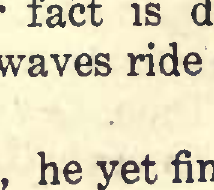
\includegraphics[width=0.8\textwidth]{../imagenes/pagina_027_fig_03.png}
\caption{Figura de la página 27}
\end{figure}

\begin{figure}[h!]
\centering
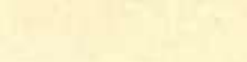
\includegraphics[width=0.8\textwidth]{../imagenes/pagina_027_fig_04.png}
\caption{Figura de la página 27}
\end{figure}

them as unerringly as he can name different sing- ers with whose tones he is acquainted. He becomes curious to know the reason, or rea- sons, for the infinite tone-peculiarity of that wond- erful musical instrument called 'Violin." By observation, he finds its G and D strings sometimes possess the bass tone-character; at an- other time these strings possess a baritone-tenor* character; in some instances A and E strings pos- sess mezzo-soprano character; in other instances A and.E strings possess soprano tone-character alone. Because of these tone peculiarities he divides violins into four classes, thus: 1. Basso-mezzo-soprano. 2. Basso-soprano. 3. Baritone-mezzo-soprano. . 4. Baritone-soprano. By experiment, he finds that these four classes of tone-character can be given to violins at will; and that they are dependent upon various degrees of .soundingrboard thicknesses, together with such tone-modifiers as size and position of exits, air capacity of the violin, etc. From observation he finds a field of usefulness peculiar to two of these classes. Thus: The vio- lin of basso-mezzo-soprano tone-character is the more agreeable solo instrument, while the baritone soprano tone-character is decidedly the more effec- tive for orchestra uses; that the latter fact is due to high tone-pitch, therefore its tone- waves ride on the topmost wave of harmony parts. Surprising as are these peculiarities, he yet finds

19

\begin{figure}[h!]
\centering

\includegraphics[width=0.8\textwidth]{../imagenes/pagina_028_fig_01.png}
\caption{Figura de la página 28}
\end{figure}

\begin{figure}[h!]
\centering
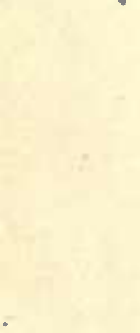
\includegraphics[width=0.8\textwidth]{../imagenes/pagina_028_fig_02.png}
\caption{Figura de la página 28}
\end{figure}

\begin{figure}[h!]
\centering
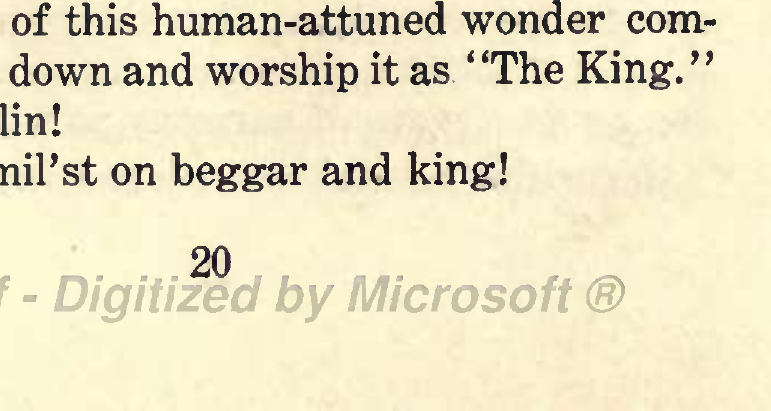
\includegraphics[width=0.8\textwidth]{../imagenes/pagina_028_fig_03.png}
\caption{Figura de la página 28}
\end{figure}

\begin{figure}[h!]
\centering
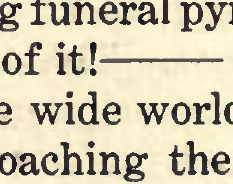
\includegraphics[width=0.8\textwidth]{../imagenes/pagina_028_fig_04.png}
\caption{Figura de la página 28}
\end{figure}

\begin{figure}[h!]
\centering
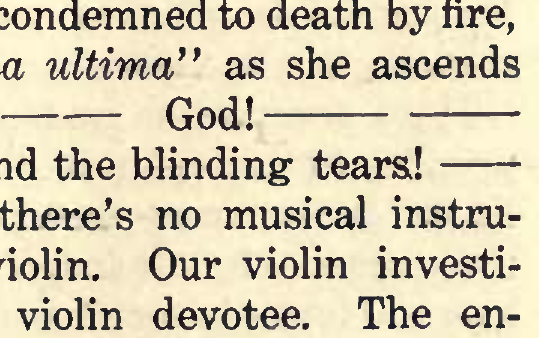
\includegraphics[width=0.8\textwidth]{../imagenes/pagina_028_fig_05.png}
\caption{Figura de la página 28}
\end{figure}

\begin{figure}[h!]
\centering
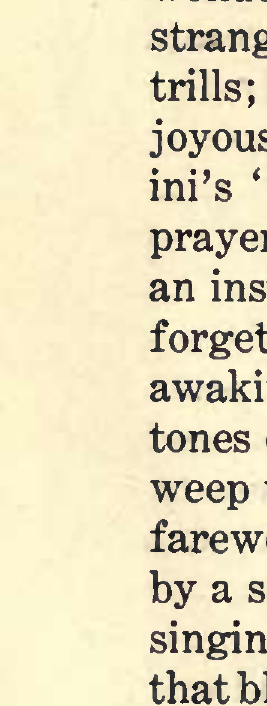
\includegraphics[width=0.8\textwidth]{../imagenes/pagina_028_fig_06.png}
\caption{Figura de la página 28}
\end{figure}

\begin{figure}[h!]
\centering
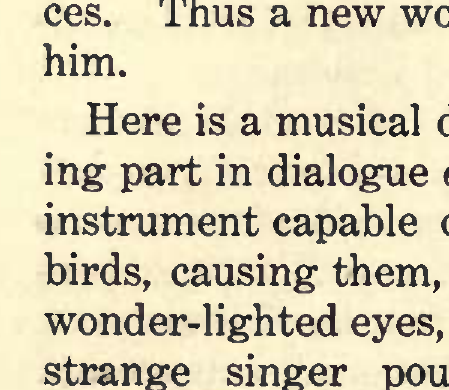
\includegraphics[width=0.8\textwidth]{../imagenes/pagina_028_fig_07.png}
\caption{Figura de la página 28}
\end{figure}

\begin{figure}[h!]
\centering
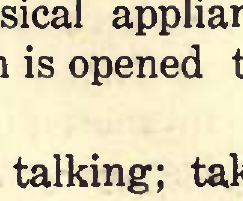
\includegraphics[width=0.8\textwidth]{../imagenes/pagina_028_fig_08.png}
\caption{Figura de la página 28}
\end{figure}

\begin{figure}[h!]
\centering
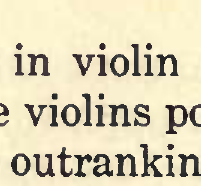
\includegraphics[width=0.8\textwidth]{../imagenes/pagina_028_fig_09.png}
\caption{Figura de la página 28}
\end{figure}

\begin{figure}[h!]
\centering
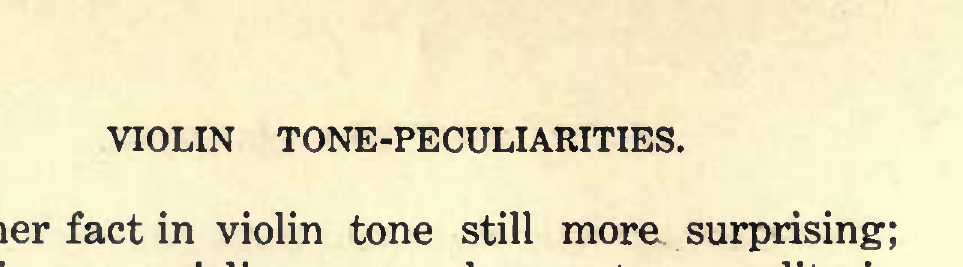
\includegraphics[width=0.8\textwidth]{../imagenes/pagina_028_fig_10.png}
\caption{Figura de la página 28}
\end{figure}

\section{VIOLIN TONE-PECULIARITIES.}

another fact in violin tone still more surprising; that is, some violins possess human tone-quality in a degree far outranking all other musical applian- ces. Thus a new world of expression is opened to him. Here is a musical device capable of talking; tak- ing part in dialogue a la "Arkansas Traveler" an instrument capable of arresting the song of wild birds, causing them, with outstretched necks and wonder-lighted eyes, to look about for that other strange singer pouring forth those enchanting trills; an instrument capable of breaking out into joyous laughter a la the laughter score in Pagan- ini's "Carnival;" an instrument capable of uttering prayer devout in Mozart's "Song Without Words;" an instrument thrilling the air with those trouble- forgetting tones in Schuman's "Traumerei;"anon, awaking human tenderness with sympathetic tones of "Sweet Home;" anon, making human eyes weep with those matchless, touching, despairing, farewell tones, as brave, loving, unfaltering Norma, by a stern Druid father condemned to death by fire, singing in "duetto e scena ultima" as she ascends that blazing funeral pyre God! the agony of it! and the blinding tears.! In all the wide world there's no musical instru- ment approaching the violin. Our violin investi- gator is now become a violin devotee. The en- trancing tones of this human-attuned wonder com- pel him to bow down and worship it as ' 'The King. " Thou, Violin! Thou that smil'st on beggar and king!

20

\begin{figure}[h!]
\centering
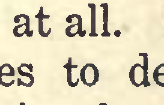
\includegraphics[width=0.8\textwidth]{../imagenes/pagina_029_fig_01.png}
\caption{Figura de la página 29}
\end{figure}

\begin{figure}[h!]
\centering
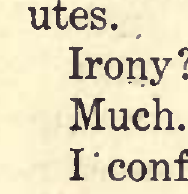
\includegraphics[width=0.8\textwidth]{../imagenes/pagina_029_fig_02.png}
\caption{Figura de la página 29}
\end{figure}

\begin{figure}[h!]
\centering
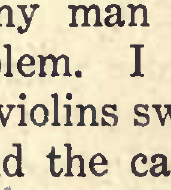
\includegraphics[width=0.8\textwidth]{../imagenes/pagina_029_fig_03.png}
\caption{Figura de la página 29}
\end{figure}

\begin{figure}[h!]
\centering
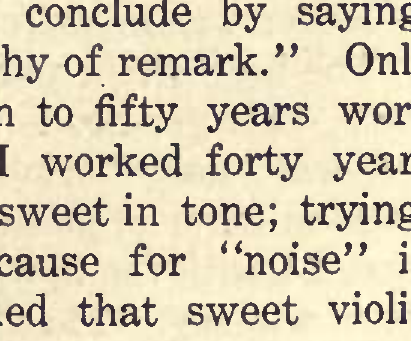
\includegraphics[width=0.8\textwidth]{../imagenes/pagina_029_fig_04.png}
\caption{Figura de la página 29}
\end{figure}

\begin{figure}[h!]
\centering
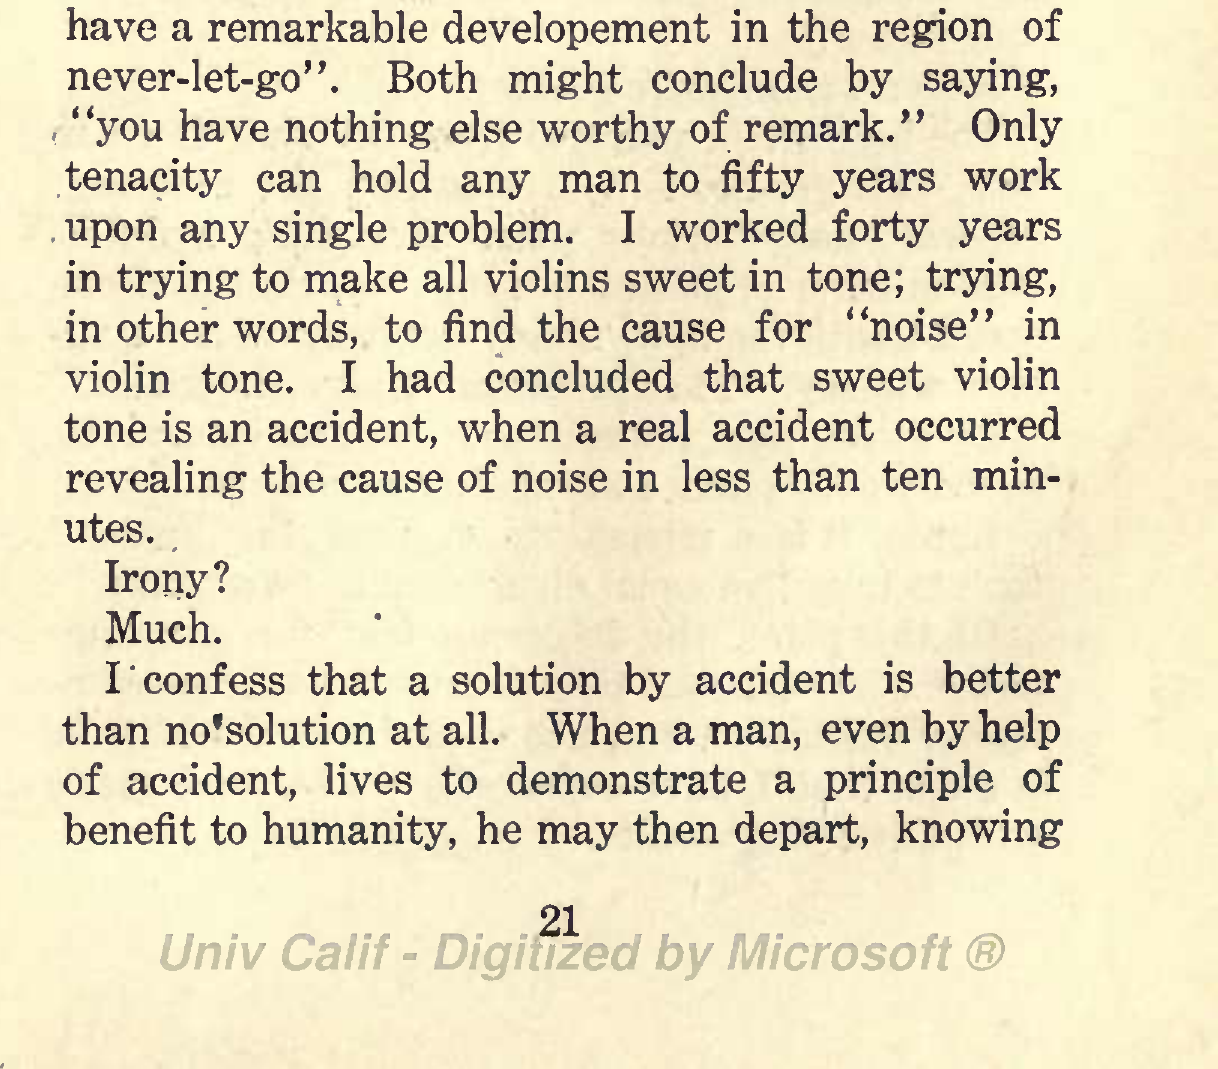
\includegraphics[width=0.8\textwidth]{../imagenes/pagina_029_fig_05.png}
\caption{Figura de la página 29}
\end{figure}

\begin{figure}[h!]
\centering
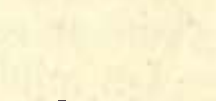
\includegraphics[width=0.8\textwidth]{../imagenes/pagina_029_fig_06.png}
\caption{Figura de la página 29}
\end{figure}

\begin{figure}[h!]
\centering
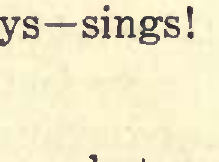
\includegraphics[width=0.8\textwidth]{../imagenes/pagina_029_fig_07.png}
\caption{Figura de la página 29}
\end{figure}

\begin{figure}[h!]
\centering
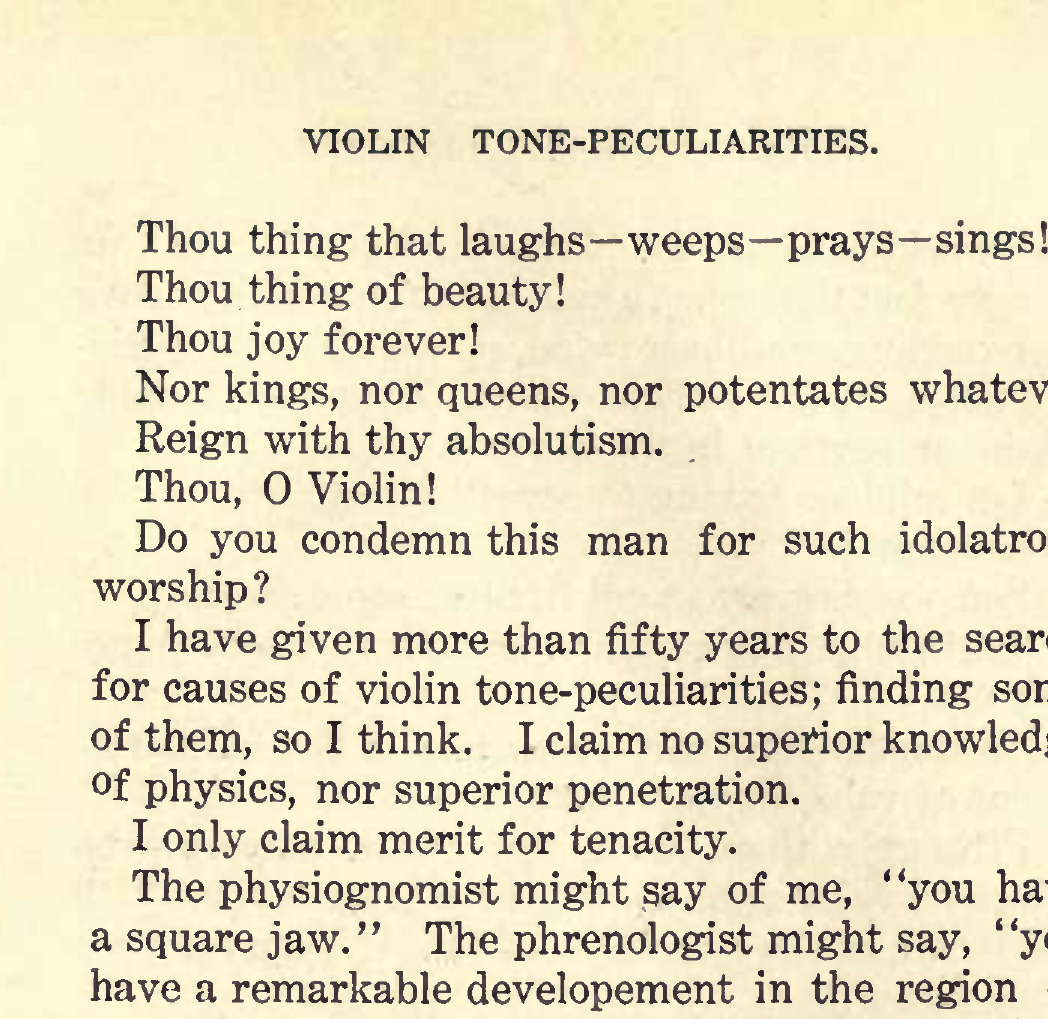
\includegraphics[width=0.8\textwidth]{../imagenes/pagina_029_fig_08.png}
\caption{Figura de la página 29}
\end{figure}

\section{VIOLIN TONE-PECULIARITIES.}

Thou thing that laughs weeps prays sings! Thou thing of beauty! Thou joy forever! Nor kings, nor queens, nor potentates whatever Reign with thy absolutism. Thou, Violin! Do you condemn this man for such idolatrous worship? I have given more than fifty years to the search for causes of violin tone-peculiarities; finding some of them, so I think. I claim no superior knowledge of physics, nor superior penetration. I only claim merit for tenacity. The physiognomist might say of me, ' 'you have a square jaw." The phrenologist might say, "you have a remarkable developement in the region of never-let-go". Both might conclude by saying, "you have nothing else worthy of remark." Only , tenacity can hold any man to fifty years work upon any single problem. I worked forty years in trying to make all violins sweet in tone; trying, in other words, to find the cause for "noise" in violin tone. I had concluded that sweet violin tone is an accident, when a real accident occurred revealing the cause of noise in less than ten min- utes. Irony? Much. I 'confess that a solution by accident is better than no'solution at all. When a man, even by help of accident, lives to demonstrate a principle of benefit to humanity, he may then depart, knowing

21

\begin{figure}[h!]
\centering
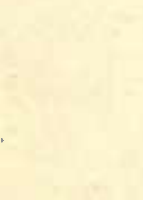
\includegraphics[width=0.8\textwidth]{../imagenes/pagina_030_fig_01.png}
\caption{Figura de la página 30}
\end{figure}

\begin{figure}[h!]
\centering
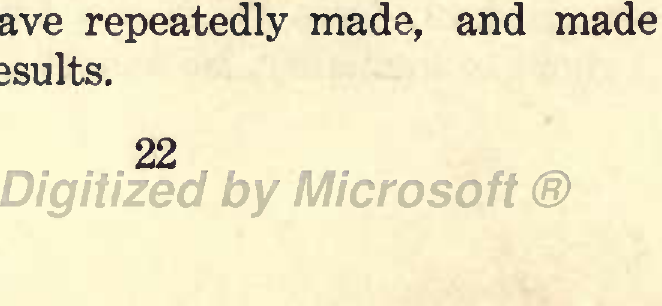
\includegraphics[width=0.8\textwidth]{../imagenes/pagina_030_fig_02.png}
\caption{Figura de la página 30}
\end{figure}

\begin{figure}[h!]
\centering
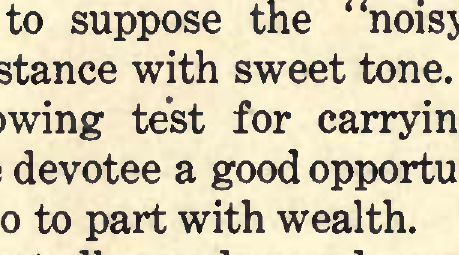
\includegraphics[width=0.8\textwidth]{../imagenes/pagina_030_fig_03.png}
\caption{Figura de la página 30}
\end{figure}

\begin{figure}[h!]
\centering
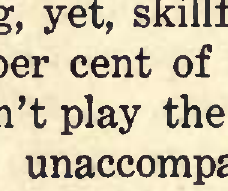
\includegraphics[width=0.8\textwidth]{../imagenes/pagina_030_fig_04.png}
\caption{Figura de la página 30}
\end{figure}

\begin{figure}[h!]
\centering
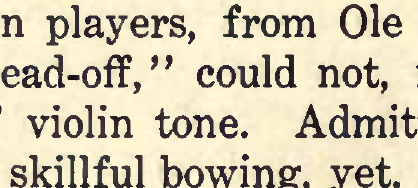
\includegraphics[width=0.8\textwidth]{../imagenes/pagina_030_fig_05.png}
\caption{Figura de la página 30}
\end{figure}

\begin{figure}[h!]
\centering
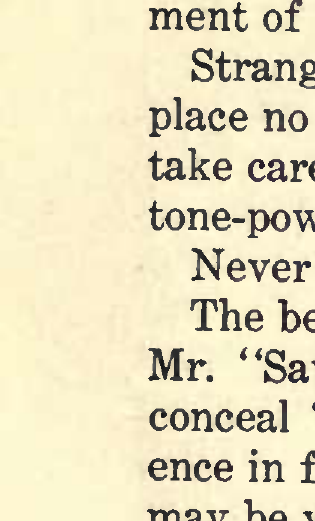
\includegraphics[width=0.8\textwidth]{../imagenes/pagina_030_fig_06.png}
\caption{Figura de la página 30}
\end{figure}

\begin{figure}[h!]
\centering
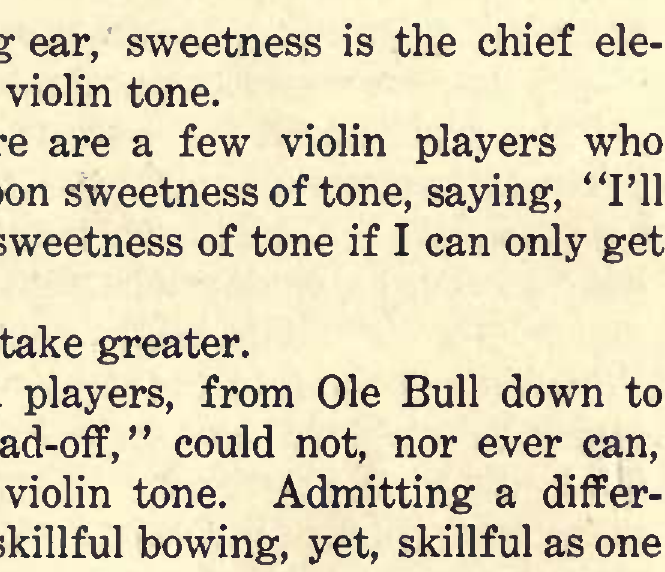
\includegraphics[width=0.8\textwidth]{../imagenes/pagina_030_fig_07.png}
\caption{Figura de la página 30}
\end{figure}

\begin{figure}[h!]
\centering
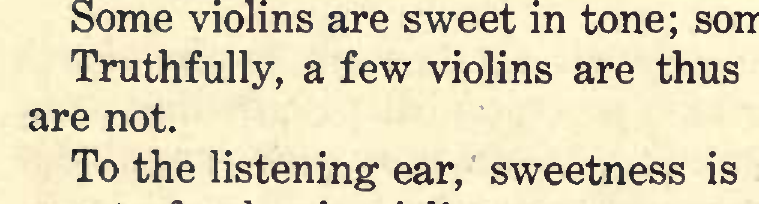
\includegraphics[width=0.8\textwidth]{../imagenes/pagina_030_fig_08.png}
\caption{Figura de la página 30}
\end{figure}

\begin{figure}[h!]
\centering
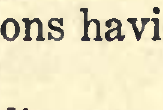
\includegraphics[width=0.8\textwidth]{../imagenes/pagina_030_fig_09.png}
\caption{Figura de la página 30}
\end{figure}

\begin{figure}[h!]
\centering
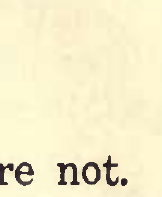
\includegraphics[width=0.8\textwidth]{../imagenes/pagina_030_fig_10.png}
\caption{Figura de la página 30}
\end{figure}

\begin{figure}[h!]
\centering
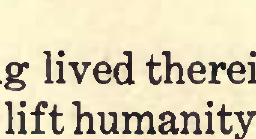
\includegraphics[width=0.8\textwidth]{../imagenes/pagina_030_fig_11.png}
\caption{Figura de la página 30}
\end{figure}

\begin{figure}[h!]
\centering
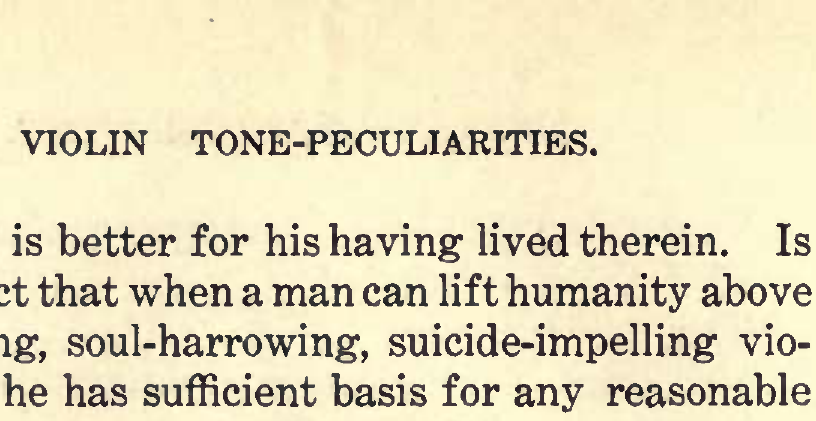
\includegraphics[width=0.8\textwidth]{../imagenes/pagina_030_fig_12.png}
\caption{Figura de la página 30}
\end{figure}

\begin{figure}[h!]
\centering
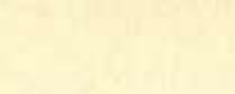
\includegraphics[width=0.8\textwidth]{../imagenes/pagina_030_fig_13.png}
\caption{Figura de la página 30}
\end{figure}

\begin{figure}[h!]
\centering
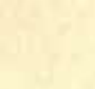
\includegraphics[width=0.8\textwidth]{../imagenes/pagina_030_fig_14.png}
\caption{Figura de la página 30}
\end{figure}

\section{VIOLIN TONE-PECULIARITIES.}

the world is better for his having lived therein. Is it not a fact that when a man can lift humanity above ear-rending, soul-harrowing, suicide-impelling vio- lin noise, he has sufficient basis for any reasonable claim on earth or in the heavens?. Let millions having "nerves" attest. Enough! Some violins are sweet in tone; some are not. Truthfully, a few violins are thus sweet; many are not. To the listening ear, sweetness is the chief ele- ment of value in violin tone. Strangely, there are a few violin players who place no value upon sweetness of tone, saying, "I'll take care of the sweetness of tone if I can only get tone-power." Never was mistake greater. The best violin players, from Ole Bull down to Mr. "Saw-yer-head-off " could not, nor ever can, conceal "noisy" violin , tone. Admitting a differ- ence in favor of skillful bowing, yet, skillful as one may be with the bow, ninety per cent of an audi- ence will say, "That fellow can't play the violin." By sweet tone I mean tone unaccompanied by sound-waves pitched at inharmonious keys. Again, it is a mistake to suppose the "noisy" tone to travel an equal distance with sweet tone. On this point, the following test for carrying- power gives the loud tone devotee a good opportun- ity for disillusion, and also to part with wealth. It is a test that I have repeatedly made, and made with unvarying results.

22

\begin{figure}[h!]
\centering
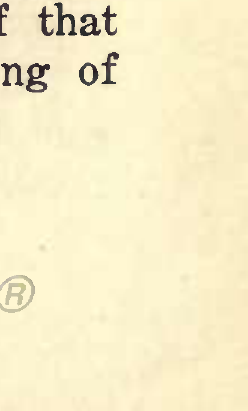
\includegraphics[width=0.8\textwidth]{../imagenes/pagina_031_fig_01.png}
\caption{Figura de la página 31}
\end{figure}

\begin{figure}[h!]
\centering
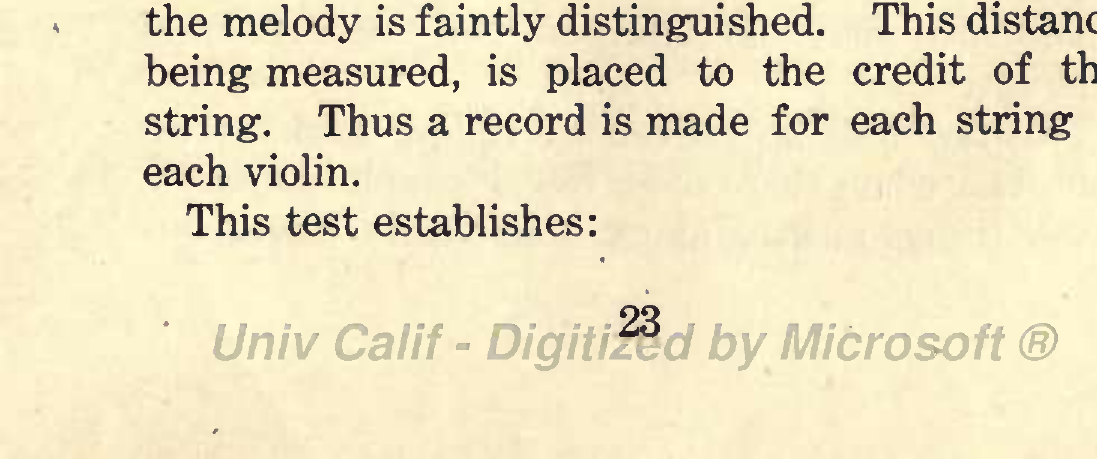
\includegraphics[width=0.8\textwidth]{../imagenes/pagina_031_fig_02.png}
\caption{Figura de la página 31}
\end{figure}

\begin{figure}[h!]
\centering
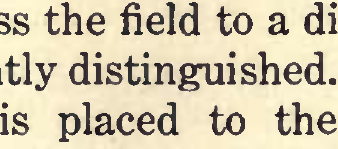
\includegraphics[width=0.8\textwidth]{../imagenes/pagina_031_fig_03.png}
\caption{Figura de la página 31}
\end{figure}

\begin{figure}[h!]
\centering
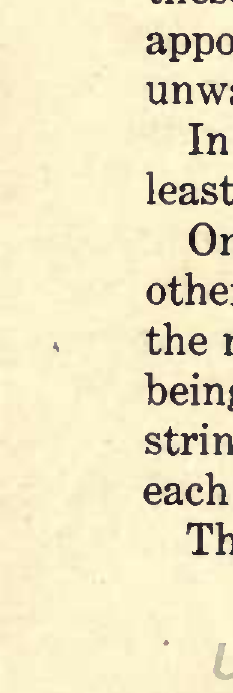
\includegraphics[width=0.8\textwidth]{../imagenes/pagina_031_fig_04.png}
\caption{Figura de la página 31}
\end{figure}

\begin{figure}[h!]
\centering
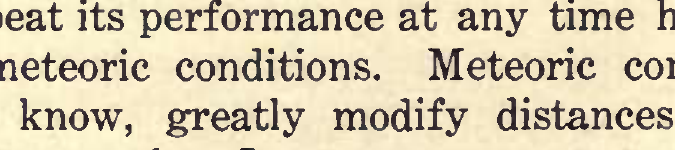
\includegraphics[width=0.8\textwidth]{../imagenes/pagina_031_fig_05.png}
\caption{Figura de la página 31}
\end{figure}

\begin{figure}[h!]
\centering
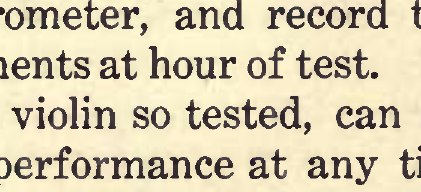
\includegraphics[width=0.8\textwidth]{../imagenes/pagina_031_fig_06.png}
\caption{Figura de la página 31}
\end{figure}

\begin{figure}[h!]
\centering
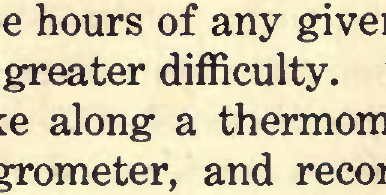
\includegraphics[width=0.8\textwidth]{../imagenes/pagina_031_fig_07.png}
\caption{Figura de la página 31}
\end{figure}

\begin{figure}[h!]
\centering
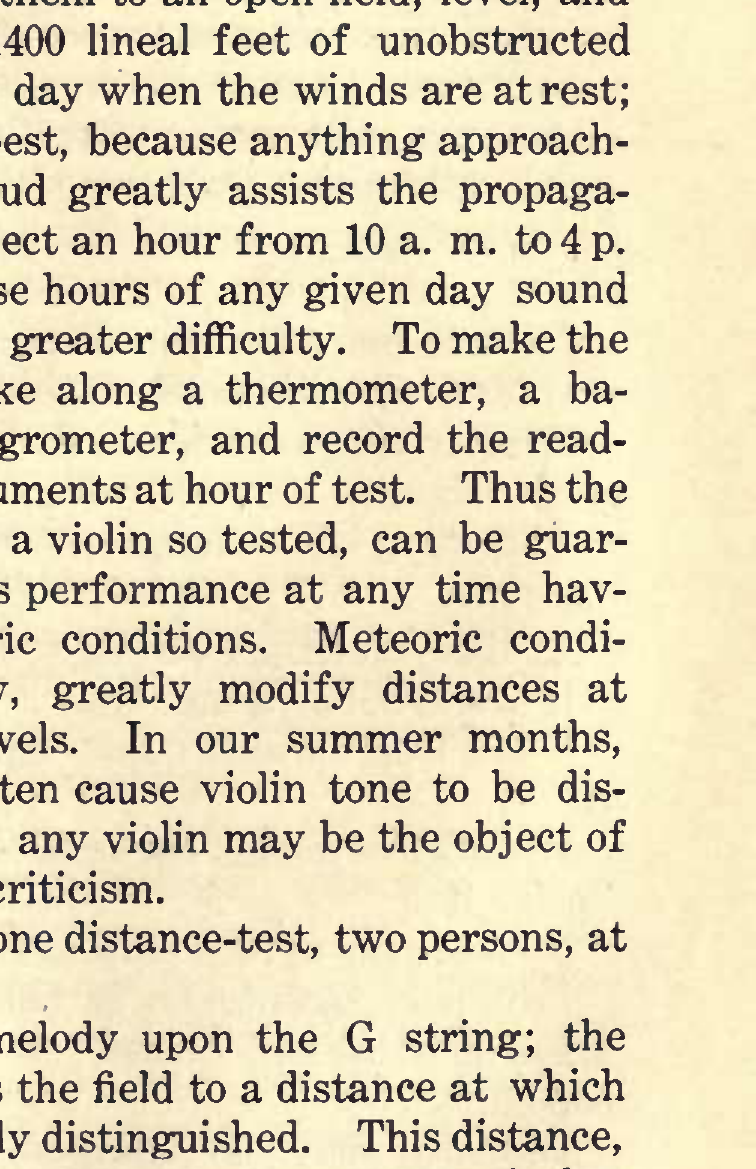
\includegraphics[width=0.8\textwidth]{../imagenes/pagina_031_fig_08.png}
\caption{Figura de la página 31}
\end{figure}

\begin{figure}[h!]
\centering
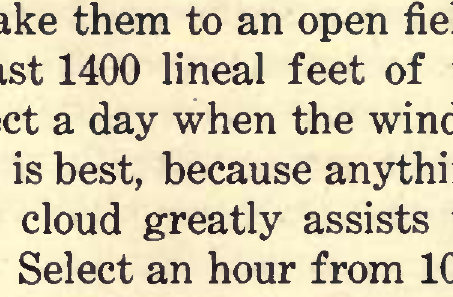
\includegraphics[width=0.8\textwidth]{../imagenes/pagina_031_fig_09.png}
\caption{Figura de la página 31}
\end{figure}

\begin{figure}[h!]
\centering
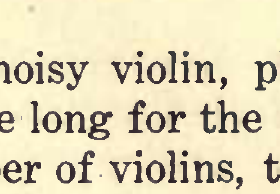
\includegraphics[width=0.8\textwidth]{../imagenes/pagina_031_fig_10.png}
\caption{Figura de la página 31}
\end{figure}

\begin{figure}[h!]
\centering
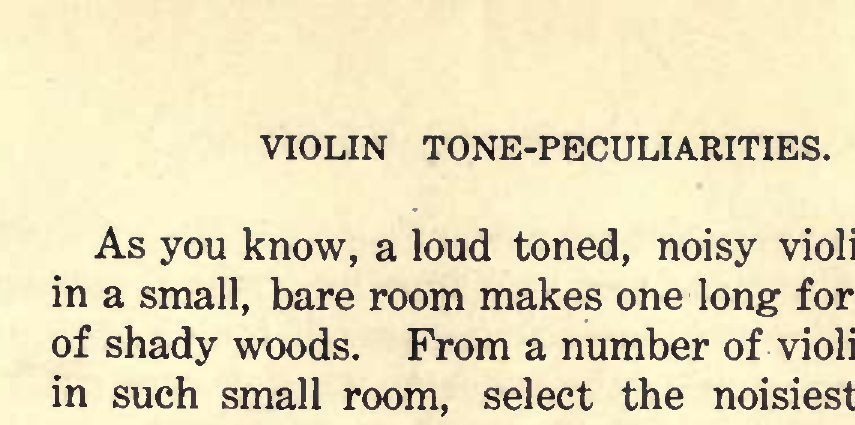
\includegraphics[width=0.8\textwidth]{../imagenes/pagina_031_fig_11.png}
\caption{Figura de la página 31}
\end{figure}

\section{VIOLIN TONE-PECULIARITIES.}

As you know, a loud toned, noisy violin, played in a small, bare room makes one long for the quiet of shady woods. From a number of violins, tested in such small room, select the noisiest and the sweetest and take them to an open field, level, and affording at least 1400 lineal feet of unobstructed distance. Select a day when the winds are at rest; a cloudless day is best, because anything approach- ing the nimbus cloud greatly assists the propaga- tion of sound. Select an hour from 10 a. m. to 4 p. m., because in those hours of any given day sound is propagated with greater difficulty. To make the record of value, take along a thermometer, a ba- rometer, and a hygrometer, and record the read- ings of these instruments at hour of test. Thus the carrying power, of a violin so tested, can be guar- anteed to repeat its performance at any time hav- ing similar meteoric conditions. Meteoric condi- tions, as you know, greatly modify distances at which sounds travels. In our summer months, these conditions often cause violin tone to be dis- appointing. Thus, any violin may be the object of unwarranted tone-criticism. In making this tone distance-test, two persons, at least, must assist. One will play a melody upon the G string; the other retires across the field to a distance at which the melody is faintly distinguished. This distance, being measured, is placed to the credit of that string. Thus a record is made for each string of each violin. This test establishes:

23

\begin{figure}[h!]
\centering
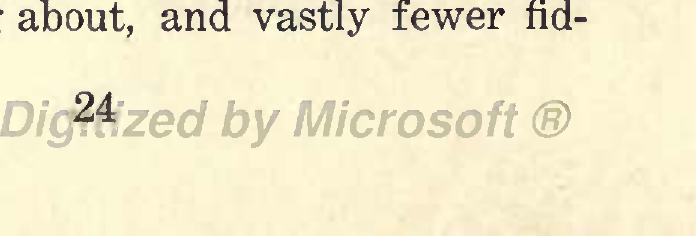
\includegraphics[width=0.8\textwidth]{../imagenes/pagina_032_fig_01.png}
\caption{Figura de la página 32}
\end{figure}

\begin{figure}[h!]
\centering
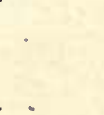
\includegraphics[width=0.8\textwidth]{../imagenes/pagina_032_fig_02.png}
\caption{Figura de la página 32}
\end{figure}

\begin{figure}[h!]
\centering
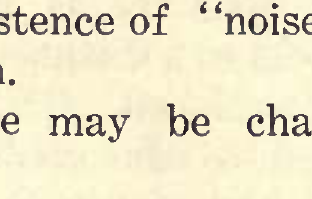
\includegraphics[width=0.8\textwidth]{../imagenes/pagina_032_fig_03.png}
\caption{Figura de la página 32}
\end{figure}

\begin{figure}[h!]
\centering
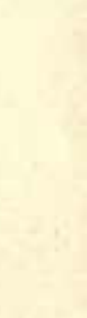
\includegraphics[width=0.8\textwidth]{../imagenes/pagina_032_fig_04.png}
\caption{Figura de la página 32}
\end{figure}

\begin{figure}[h!]
\centering
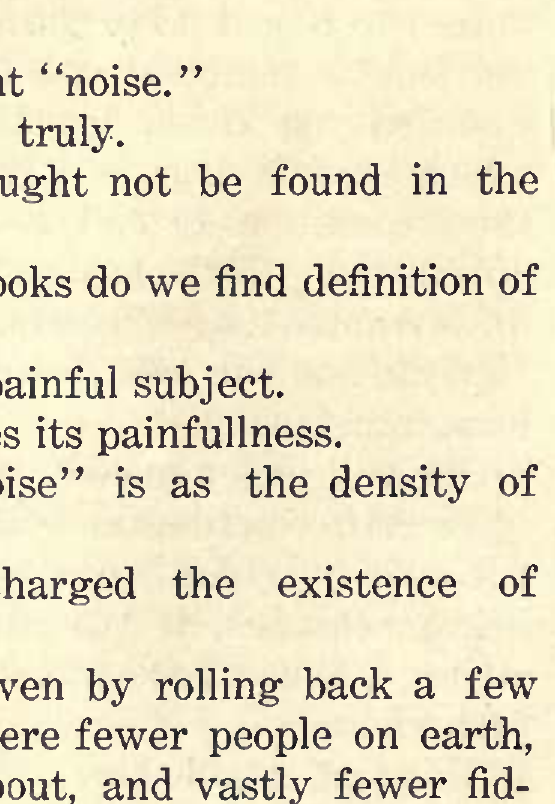
\includegraphics[width=0.8\textwidth]{../imagenes/pagina_032_fig_05.png}
\caption{Figura de la página 32}
\end{figure}

\begin{figure}[h!]
\centering
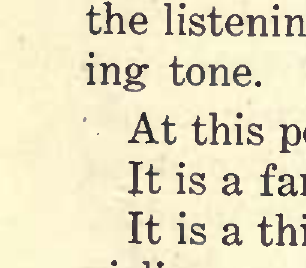
\includegraphics[width=0.8\textwidth]{../imagenes/pagina_032_fig_06.png}
\caption{Figura de la página 32}
\end{figure}

\begin{figure}[h!]
\centering
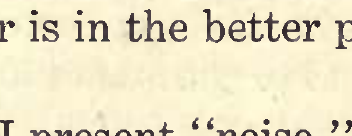
\includegraphics[width=0.8\textwidth]{../imagenes/pagina_032_fig_07.png}
\caption{Figura de la página 32}
\end{figure}

\begin{figure}[h!]
\centering
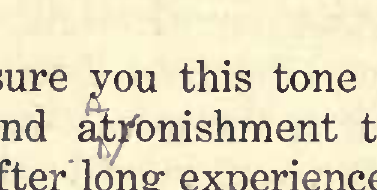
\includegraphics[width=0.8\textwidth]{../imagenes/pagina_032_fig_08.png}
\caption{Figura de la página 32}
\end{figure}

\begin{figure}[h!]
\centering
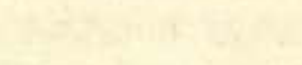
\includegraphics[width=0.8\textwidth]{../imagenes/pagina_032_fig_09.png}
\caption{Figura de la página 32}
\end{figure}

\begin{figure}[h!]
\centering
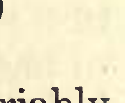
\includegraphics[width=0.8\textwidth]{../imagenes/pagina_032_fig_10.png}
\caption{Figura de la página 32}
\end{figure}

\begin{figure}[h!]
\centering
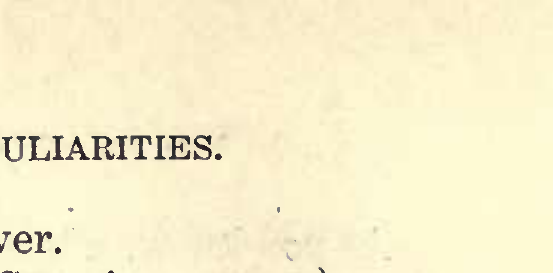
\includegraphics[width=0.8\textwidth]{../imagenes/pagina_032_fig_11.png}
\caption{Figura de la página 32}
\end{figure}

\begin{figure}[h!]
\centering
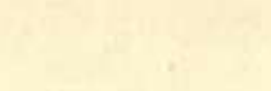
\includegraphics[width=0.8\textwidth]{../imagenes/pagina_032_fig_12.png}
\caption{Figura de la página 32}
\end{figure}

\section{VIOLIN TONE-PECULIARITIES.}

(1) Evenness of tone power. (2) Intensity of tone. (Carrying power.) (3) Purity of tone. (Sweetness of tone.) In my experience, the sweeter tone invariably travels the greater distance. I have known the sweeter toned violin to win by 250 feet. In even- ness of tone, I tested one reputable old violin whose distance record\textasciicircum\{\} varies from G string 1000, to E string, 1480 feet. Only two violins have I thus test- ed, securing an equal distance-record for each

string. I assure you this tone distance-test may cause profound admonishment to the participants. My- self, after long experience, dare not risk anything on the result. This test affords ample proof that the listening ear is in the better position for judg- ing tone. At this point I present "noise." It is a familiar thing, truly. It is a thing which ought not be found in the violin. Not always in text books do we find definition of "noise." Noise seems to be a painful subject. Proximity accentuates its painfullness. The existence of "noise" is as the density of population. To noise may be charged the existence of "nerves." This fact may be proven by rolling back a few centuries when there were fewer people on earth, fewer things moving about, and vastly fewer fid-

24

\begin{figure}[h!]
\centering
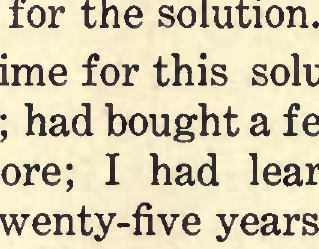
\includegraphics[width=0.8\textwidth]{../imagenes/pagina_033_fig_01.png}
\caption{Figura de la página 33}
\end{figure}

\begin{figure}[h!]
\centering
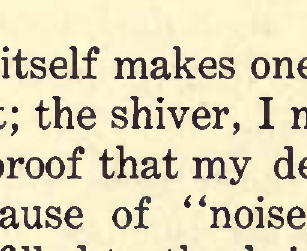
\includegraphics[width=0.8\textwidth]{../imagenes/pagina_033_fig_02.png}
\caption{Figura de la página 33}
\end{figure}

\begin{figure}[h!]
\centering
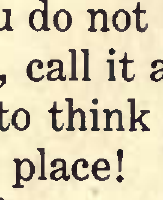
\includegraphics[width=0.8\textwidth]{../imagenes/pagina_033_fig_03.png}
\caption{Figura de la página 33}
\end{figure}

\begin{figure}[h!]
\centering
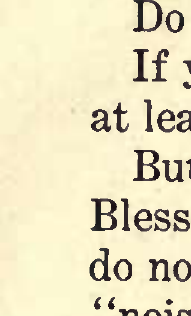
\includegraphics[width=0.8\textwidth]{../imagenes/pagina_033_fig_04.png}
\caption{Figura de la página 33}
\end{figure}

\section{VIOLIN TONE-PECULIARITIES.}

dlers, and there we find no record of "nerves." Science would have us believe that where there are no ears, there is no sound, no "noise." Do you believe this story? If you do not care to express disbelief you may, at least, call it a paradox. But, to think of a place where there's no noise! Blessed place! That must be a place where angels do not fear to tread. Let it not be invaded by the "noisy" violin, for the most distracting noise, noise "le plus terrible," can come from the violin. What is noise? Should you not find a definition to suit you, read the following: Noise is an aggre- gation of sound-waves pitched at inharmonious keys. The definition itself makes one shiver. I'm proud of it; the shiver, I mean. The shiver is proof that my definition is correct. What is the cause of "noise" in violin tone? This question is filled to the brim with absorbing interest to the whole violin world. The accident, affording a solution to this mo- mentous question, is so provokingly accidental as to rob me of all honor for the solution. I had worked a lifetime for this solution; I had read books, and books; had bought a few books my- self; had borrowed more; I had learned therein some facts requiring twenty-five years to unlearn; I had given up the possibility of a solution, believ- ing sweetness of violin tone to be an accident, when the following accident occurred, thus:

25

\begin{figure}[h!]
\centering

\includegraphics[width=0.8\textwidth]{../imagenes/pagina_034_fig_01.png}
\caption{Figura de la página 34}
\end{figure}

\begin{figure}[h!]
\centering
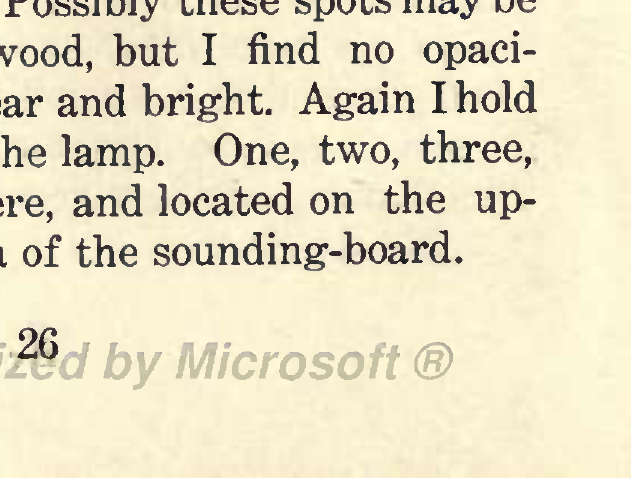
\includegraphics[width=0.8\textwidth]{../imagenes/pagina_034_fig_02.png}
\caption{Figura de la página 34}
\end{figure}

\begin{figure}[h!]
\centering
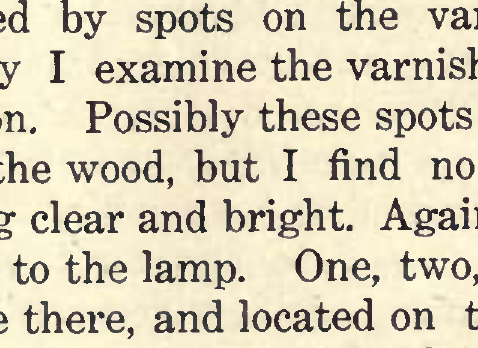
\includegraphics[width=0.8\textwidth]{../imagenes/pagina_034_fig_03.png}
\caption{Figura de la página 34}
\end{figure}

\begin{figure}[h!]
\centering
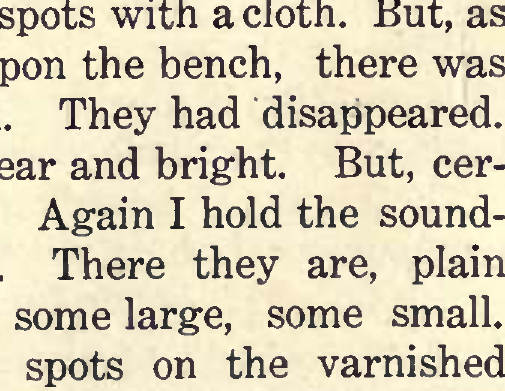
\includegraphics[width=0.8\textwidth]{../imagenes/pagina_034_fig_04.png}
\caption{Figura de la página 34}
\end{figure}

\begin{figure}[h!]
\centering
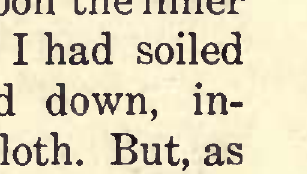
\includegraphics[width=0.8\textwidth]{../imagenes/pagina_034_fig_05.png}
\caption{Figura de la página 34}
\end{figure}

\begin{figure}[h!]
\centering
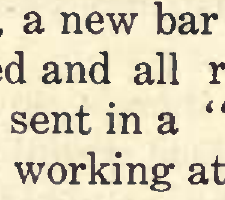
\includegraphics[width=0.8\textwidth]{../imagenes/pagina_034_fig_06.png}
\caption{Figura de la página 34}
\end{figure}

\begin{figure}[h!]
\centering
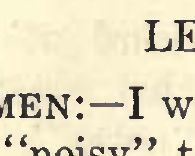
\includegraphics[width=0.8\textwidth]{../imagenes/pagina_034_fig_07.png}
\caption{Figura de la página 34}
\end{figure}

\begin{figure}[h!]
\centering
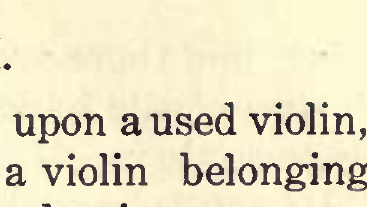
\includegraphics[width=0.8\textwidth]{../imagenes/pagina_034_fig_08.png}
\caption{Figura de la página 34}
\end{figure}

\begin{figure}[h!]
\centering
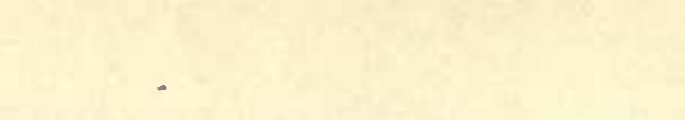
\includegraphics[width=0.8\textwidth]{../imagenes/pagina_034_fig_09.png}
\caption{Figura de la página 34}
\end{figure}

\section{VIOLIN TONE-PECULIARITIES.}

\section{LECTURE II.}

GENTLEMEN: I was working upon a used violin, a violin of "noisy" tone-faults, a violin belonging to a "business" player. Re-graduation was com- pleted, a new bar ad justed, interior surf acing- work finished and all ready for assembling when the owner sent in a "hurry up" call. To hurry up meant working at night, and to please, my friend, I resolved to do assembling work that same night. Accordingly I returned to my workroom, lighting a 20-candlepower lamp placed before a reflector and seated myself immediately in front of the lamp. Reaching to my right, I picked up the finished sounding-board. As it came between my sight and the lamp, I noticed some dark spots upon the inner surface. Thinking that in some way I had soiled the surface, I laid the sounding-board down, in- tending to remove these spots with a cloth. But, as the sounding-board lay upon the bench, there was no soiled spots to be seen. They had disappeared. The inner surface was clear and bright. But, cer- tainly I saw dark spots. Again I hold the sound- ing-board up to the lamp. There they are, plain enough; several of them; some large, some small. They must be caused by spots on the varnished surface. Critically I examine the varnish. No spots appear thereon. Possibly these spots may be due to opacities in the wood, but I find no opaci- ties; the wood being clear and bright. Again I hold the sounding-board to the lamp. One, two, three, six cloudy areas are there, and located on the up- per tone-producing area of the sounding-board.

26

\begin{figure}[h!]
\centering
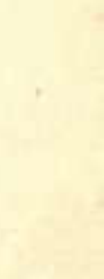
\includegraphics[width=0.8\textwidth]{../imagenes/pagina_035_fig_01.png}
\caption{Figura de la página 35}
\end{figure}

\begin{figure}[h!]
\centering
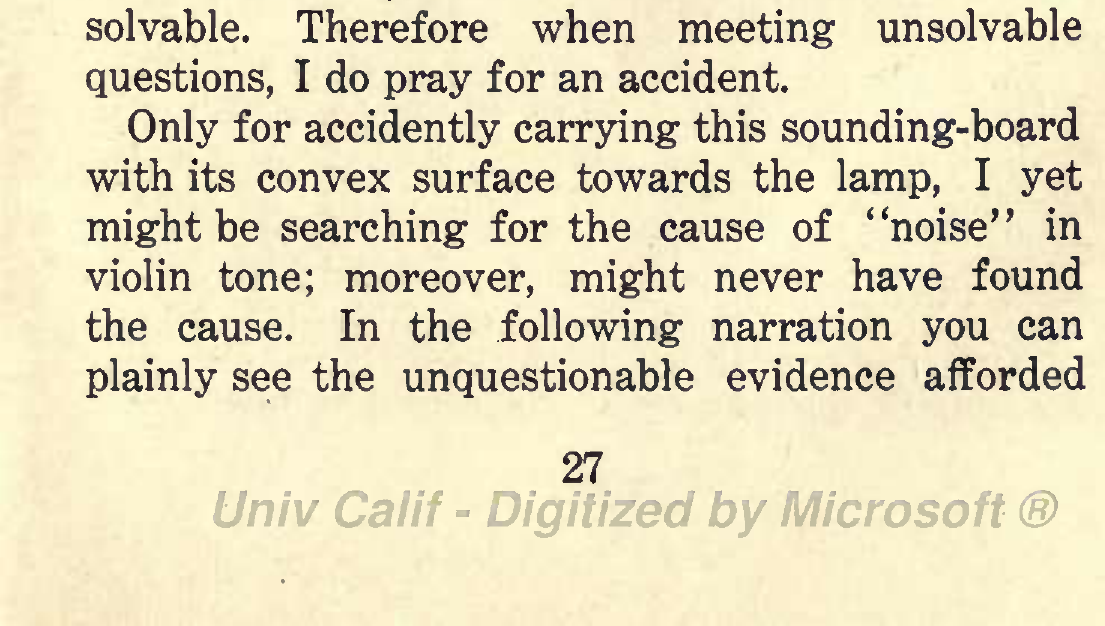
\includegraphics[width=0.8\textwidth]{../imagenes/pagina_035_fig_02.png}
\caption{Figura de la página 35}
\end{figure}

\begin{figure}[h!]
\centering
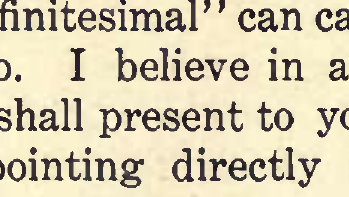
\includegraphics[width=0.8\textwidth]{../imagenes/pagina_035_fig_03.png}
\caption{Figura de la página 35}
\end{figure}

\begin{figure}[h!]
\centering
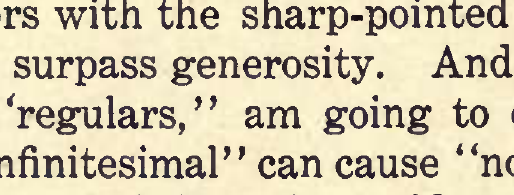
\includegraphics[width=0.8\textwidth]{../imagenes/pagina_035_fig_04.png}
\caption{Figura de la página 35}
\end{figure}

\begin{figure}[h!]
\centering
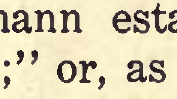
\includegraphics[width=0.8\textwidth]{../imagenes/pagina_035_fig_05.png}
\caption{Figura de la página 35}
\end{figure}

\begin{figure}[h!]
\centering
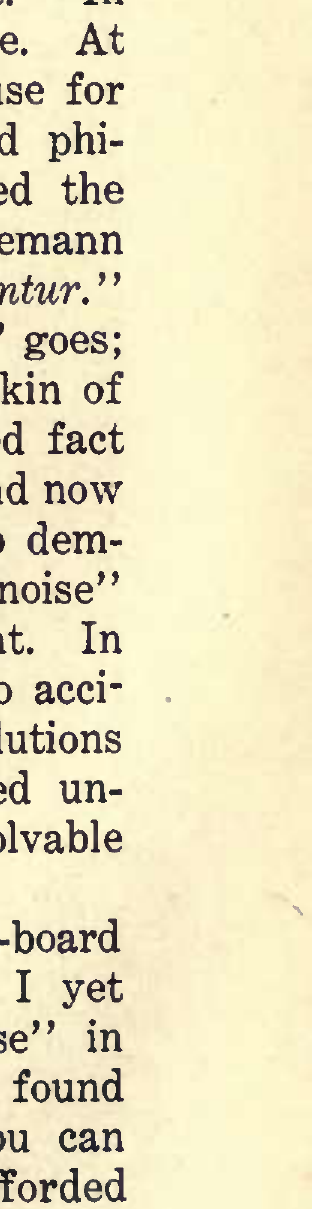
\includegraphics[width=0.8\textwidth]{../imagenes/pagina_035_fig_06.png}
\caption{Figura de la página 35}
\end{figure}

\begin{figure}[h!]
\centering
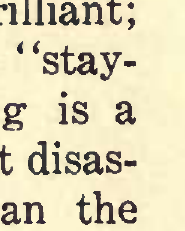
\includegraphics[width=0.8\textwidth]{../imagenes/pagina_035_fig_07.png}
\caption{Figura de la página 35}
\end{figure}

\begin{figure}[h!]
\centering
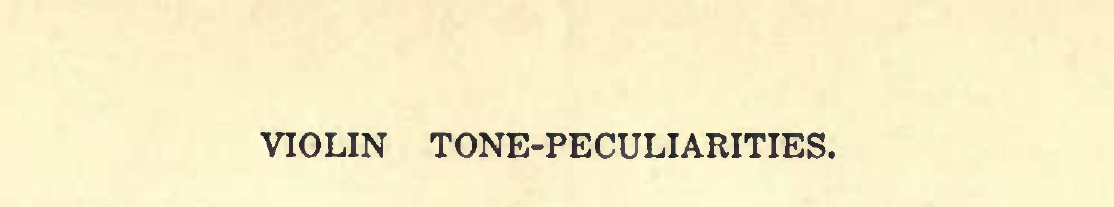
\includegraphics[width=0.8\textwidth]{../imagenes/pagina_035_fig_08.png}
\caption{Figura de la página 35}
\end{figure}

\section{VIOLIN TONE-PECULIARITIES.}

Motionless, I gaze at those cloudy areas, thinking, thinking hard for an explanation. Slowly the ex- planation came, slowly of course. I am not brilliant; never posed as a prodigy; am slow, but am a ' 'stay- er," also a smoker. As you know, smoking is a prerequisite of the philosopher. We cannot disas- sociate the pipe and the German, neither can the world match him in solving knotty problems. In imitation of the philosopher, I light my pipe. At once, through clouds of smoke, I see the cause for these cloudy areas. Thus does "smoke" aid phi- losophy. The great Hahnemann established the principle that "like cures like;" or, as Hahnemann states in choice Latin, ' 'Similia similibus curantur. ' ' I believe in Hahnemann as far as "smoke" goes; yet, that great thinker did pierce the thick skin of the "regular" doctors with the sharp-pointed fact that our doses often surpass generosity. And now myself, one of the ' 'regulars, ' ' am going to dem- onstrate that the "infinitesimal" can cause "noise" inside the violin too. I believe in accident. In due course of time I shall present to you two acci- dental occurrences pointing directly at solutions of violin tone-problems hitherto pronounced un- solvable. Therefore when meeting unsolvable questions, I do pray for an accident. Only for accidently carrying this sounding-board with its convex surface towards the lamp, I yet might be searching for the cause of "noise" in violin tone; moreover, might never have found the cause. In the following narration you can plainly see the unquestionable evidence afforded

27

\begin{figure}[h!]
\centering
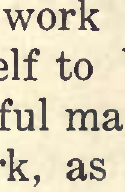
\includegraphics[width=0.8\textwidth]{../imagenes/pagina_036_fig_01.png}
\caption{Figura de la página 36}
\end{figure}

\begin{figure}[h!]
\centering
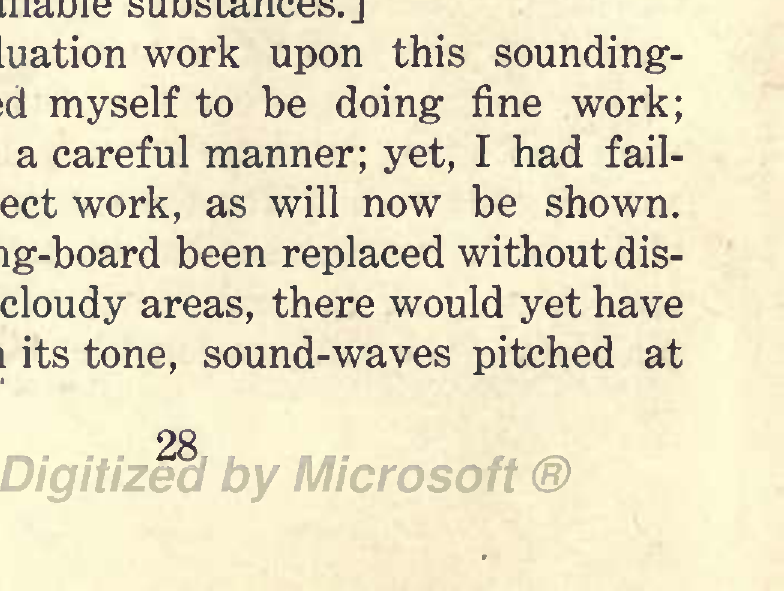
\includegraphics[width=0.8\textwidth]{../imagenes/pagina_036_fig_02.png}
\caption{Figura de la página 36}
\end{figure}

\begin{figure}[h!]
\centering
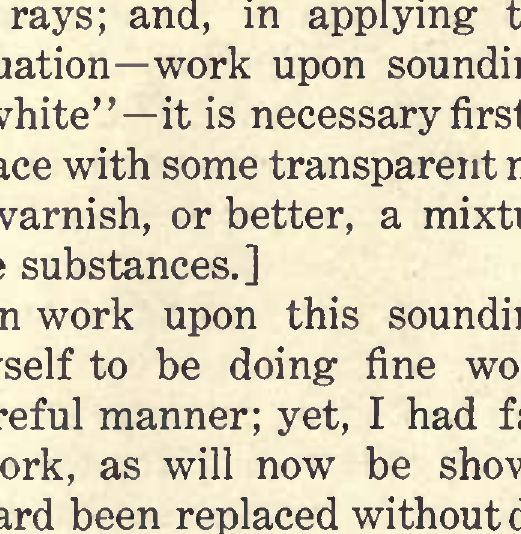
\includegraphics[width=0.8\textwidth]{../imagenes/pagina_036_fig_03.png}
\caption{Figura de la página 36}
\end{figure}

\begin{figure}[h!]
\centering
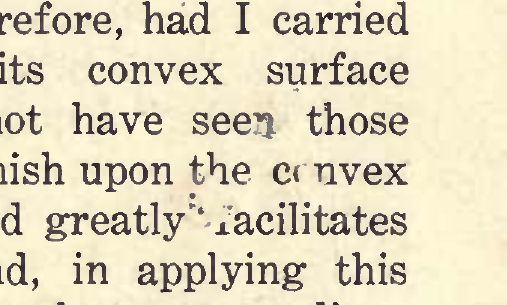
\includegraphics[width=0.8\textwidth]{../imagenes/pagina_036_fig_04.png}
\caption{Figura de la página 36}
\end{figure}

\begin{figure}[h!]
\centering
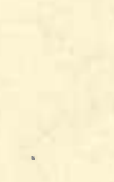
\includegraphics[width=0.8\textwidth]{../imagenes/pagina_036_fig_05.png}
\caption{Figura de la página 36}
\end{figure}

\begin{figure}[h!]
\centering
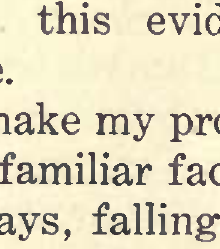
\includegraphics[width=0.8\textwidth]{../imagenes/pagina_036_fig_06.png}
\caption{Figura de la página 36}
\end{figure}

\begin{figure}[h!]
\centering
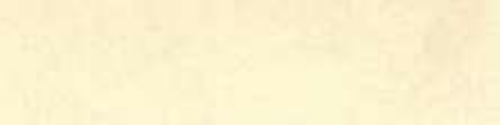
\includegraphics[width=0.8\textwidth]{../imagenes/pagina_036_fig_07.png}
\caption{Figura de la página 36}
\end{figure}

\begin{figure}[h!]
\centering
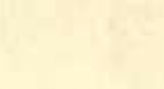
\includegraphics[width=0.8\textwidth]{../imagenes/pagina_036_fig_08.png}
\caption{Figura de la página 36}
\end{figure}

\section{VIOLIN TONE-PECULIARITIES.}

by accident, for, in the light of theories of musical sound, this evidence stands forth in clear-cut outline. To make my process of reasoning clear, I call up a few familiar facts in natural philosophy: Thus, light rays, falling upon the convex surface of a con- cavo-convex body, (as the violin sounding-board, ) after passing through such body are bent from a direct line at the moment of leaving the concave surface, and thence travel in converging lines to a focus; theiJ\textasciicircum\{\}ore, objects upon the concave surface become magnified; but, reversing the direction of travel, light rays leaving the convex surface, are dispersed; hence, objects upon the convex surface appear diminished in size; therefore, had I carried this sounding-board with its convex surface towards the lamp, I could not have seen those cloudy areas. [The clear varnish upon the C( nvex surface of this sounding-board greatly'* facilitates transmission of light rays; and, in applying this test for perfect graduation work upon sounding- board wood "in the white" it is necessary first to cover the convex surface with some transparent me- dium, as oil, or clear varnish, or better, a mixture of these two available substances.] In doing graduation work upon this sounding- board, I supposed myself to be doing fine work; using calipers in a careful manner; yet, I had fail- ed of doing perfect work, as will now be shown. Had this sounding-board been replaced without dis- covery of those cloudy areas, there would yet have been mixed with its tone, sound-waves pitched at

28

\begin{figure}[h!]
\centering

\includegraphics[width=0.8\textwidth]{../imagenes/pagina_037_fig_01.png}
\caption{Figura de la página 37}
\end{figure}

\begin{figure}[h!]
\centering
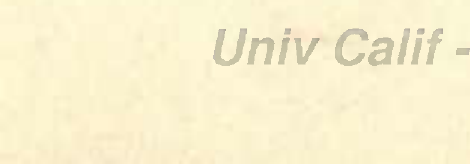
\includegraphics[width=0.8\textwidth]{../imagenes/pagina_037_fig_02.png}
\caption{Figura de la página 37}
\end{figure}

\begin{figure}[h!]
\centering
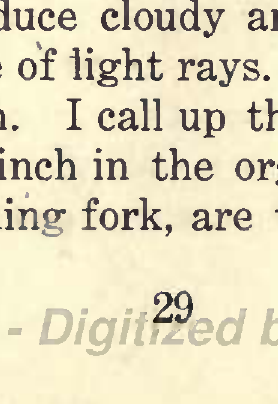
\includegraphics[width=0.8\textwidth]{../imagenes/pagina_037_fig_03.png}
\caption{Figura de la página 37}
\end{figure}

\begin{figure}[h!]
\centering
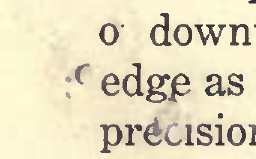
\includegraphics[width=0.8\textwidth]{../imagenes/pagina_037_fig_04.png}
\caption{Figura de la página 37}
\end{figure}

\section{VIOLIN TONE-PECULIARITIES.}

inharmonious keys or "noise." As before, hold- ing the sounding-board to the lamp, with a pencil I circumscribe one of those areas, and therein, with a scraper remove a little wood. Now, in this area, light comes through more freely. I continue thus with scraper until this circumscribed area becomes equally luminous with adjoining areas. "Qoctor, how much wood did you thus remove?" I cannot answer this question with precision; but say perhaps the 100 part of an inch in some places; in other places of deeper cloudiness, a greater amount. You must understand the form of gradu- ation applied to this sounding-board to be 9-64 inch at position of bridge; thence, in either up ward o downward direction, down to 3-32 inch at the f edge as near as practical to work. Thus, absolute precision in diminution of sounding-board thickness- es becomes a matter of difficulty; in fact, this form of sounding-board graduation is not surpassed in diffi- culty by any other form known. You must also understand that where thickness equals 9-64, but little or no light passes through; also, that great- est luminosity, on this plate, occurs at the thickness of 3-32 inch; that between these two points, lumin- osity diminishes, or increases, with a regularity exactly proportionate to diminution, or increase of sounding-board thickness; therefore, irregularities in thickness produce cloudy areas by interfering with the passage of light rays. I recall rules gov- erning tone-pitch. I call up the fact that irregu- larities of 100th inch in the organ-reed, in organ- pipe, or on a tuning 1 fork, are things inadmissable.

29

\begin{figure}[h!]
\centering

\includegraphics[width=0.8\textwidth]{../imagenes/pagina_038_fig_01.png}
\caption{Figura de la página 38}
\end{figure}

\begin{figure}[h!]
\centering
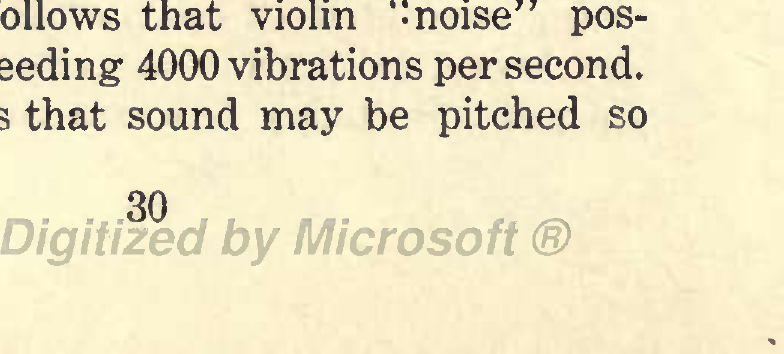
\includegraphics[width=0.8\textwidth]{../imagenes/pagina_038_fig_02.png}
\caption{Figura de la página 38}
\end{figure}

\begin{figure}[h!]
\centering
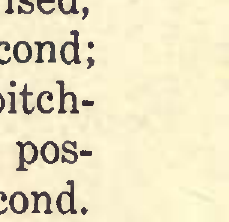
\includegraphics[width=0.8\textwidth]{../imagenes/pagina_038_fig_03.png}
\caption{Figura de la página 38}
\end{figure}

\begin{figure}[h!]
\centering
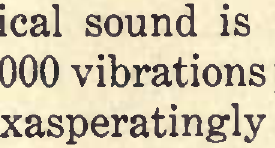
\includegraphics[width=0.8\textwidth]{../imagenes/pagina_038_fig_04.png}
\caption{Figura de la página 38}
\end{figure}

\begin{figure}[h!]
\centering
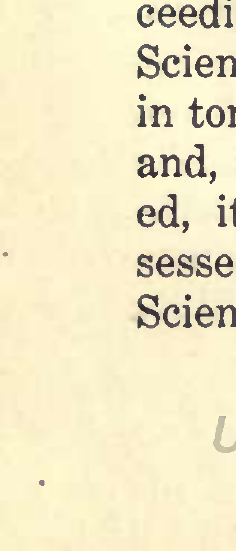
\includegraphics[width=0.8\textwidth]{../imagenes/pagina_038_fig_05.png}
\caption{Figura de la página 38}
\end{figure}

\begin{figure}[h!]
\centering
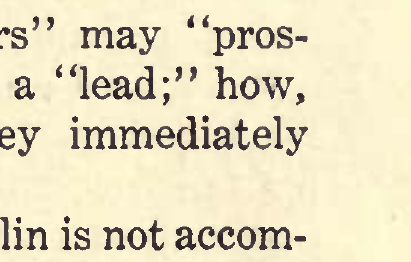
\includegraphics[width=0.8\textwidth]{../imagenes/pagina_038_fig_06.png}
\caption{Figura de la página 38}
\end{figure}

\begin{figure}[h!]
\centering
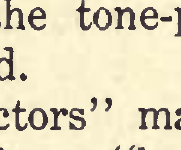
\includegraphics[width=0.8\textwidth]{../imagenes/pagina_038_fig_07.png}
\caption{Figura de la página 38}
\end{figure}

\begin{figure}[h!]
\centering
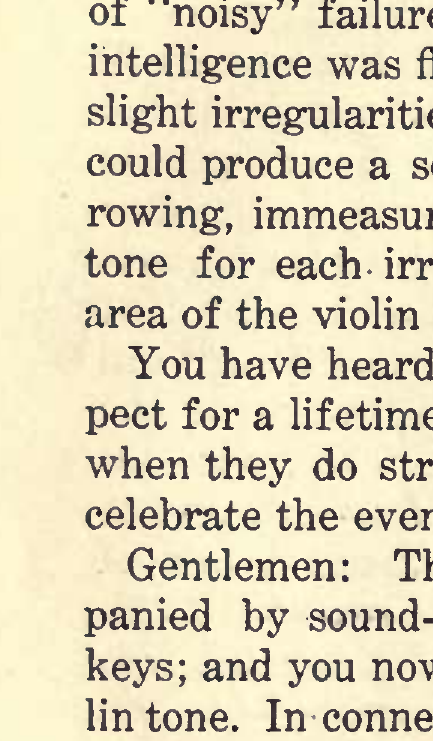
\includegraphics[width=0.8\textwidth]{../imagenes/pagina_038_fig_08.png}
\caption{Figura de la página 38}
\end{figure}

\begin{figure}[h!]
\centering
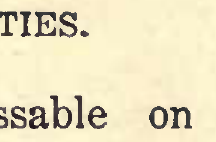
\includegraphics[width=0.8\textwidth]{../imagenes/pagina_038_fig_09.png}
\caption{Figura de la página 38}
\end{figure}

\begin{figure}[h!]
\centering
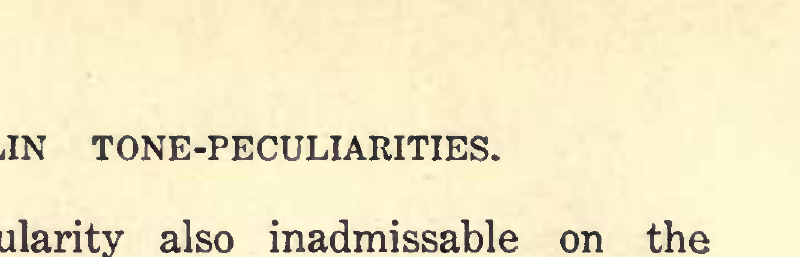
\includegraphics[width=0.8\textwidth]{../imagenes/pagina_038_fig_10.png}
\caption{Figura de la página 38}
\end{figure}

\section{VIOLIN TONE-PECULIARITIES.}

Is such irregularity also inadmissable on the violin sounding-board? Have I, at last, found the cause for "noise" in violin tone? My nerves are tingling. Forty years have I worked upon used violins trying to find a formula for eradicating "noise" therefrom; worked with the usual amount of "noisy" failure. Quicker than I can tell it, the intelligence was flashed to my sensorium that those slight irregularities of sounding-board thicknesses could produce a screaming, ear-piercing, soul-har- rowing, immeasurably high-pitched tone; one such tone for each irregularity in the tone-producing area of the violin sounding-board. You have heard how "prospectors" may "pros- pect for a lifetime without striking a "lead;" how, when they do strike a "lead" they immediately celebrate the event by going crazy. Gentlemen: The tone of this violin is not accom- panied by sound-waves pitched at inharmonious keys; and you now know the cause of "noise" in vio- lin tone. In connection with the word "violin," the word "noise" vividly recalls untold suffering; therefore, I shall press this subject upon you no further than is necessary for complete understand- ing of those high-pitched, dissonant overtones pro- ceeding from the imperfect violin sounding-board. Science states that musical sound is comprised, in tone-pitch, from 27 to 4000 vibrations per second; and, as violin "noise" is exasperatingly high-pitch- ed, it therefore follows that violin ''noise" pos- sesses a pitch exceeding 4000 vibrations per second. Science also states that sound may be pitched so

30

\begin{figure}[h!]
\centering
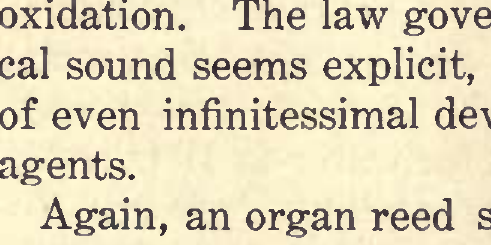
\includegraphics[width=0.8\textwidth]{../imagenes/pagina_039_fig_01.png}
\caption{Figura de la página 39}
\end{figure}

\begin{figure}[h!]
\centering
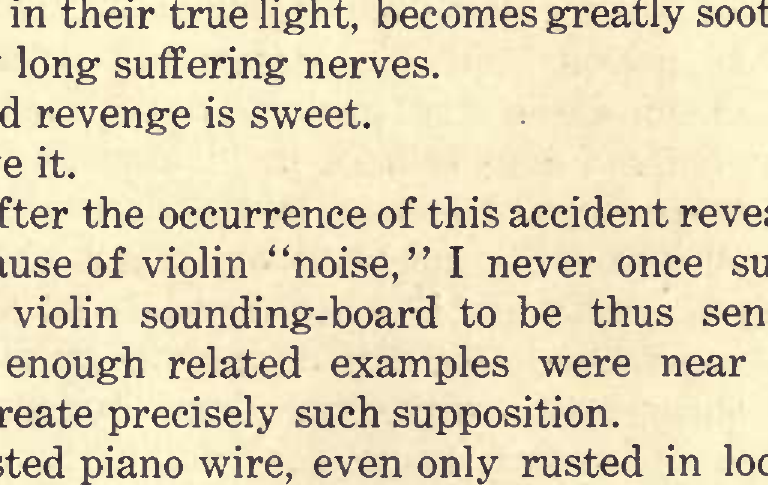
\includegraphics[width=0.8\textwidth]{../imagenes/pagina_039_fig_02.png}
\caption{Figura de la página 39}
\end{figure}

\begin{figure}[h!]
\centering
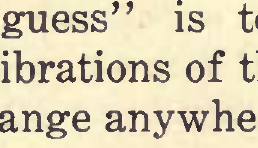
\includegraphics[width=0.8\textwidth]{../imagenes/pagina_039_fig_03.png}
\caption{Figura de la página 39}
\end{figure}

\begin{figure}[h!]
\centering
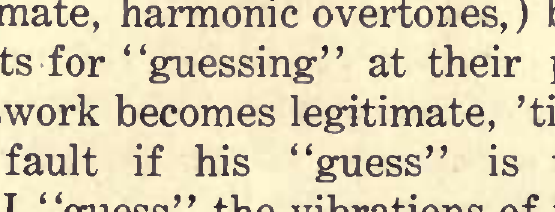
\includegraphics[width=0.8\textwidth]{../imagenes/pagina_039_fig_04.png}
\caption{Figura de la página 39}
\end{figure}

\section{VIOLIN TONE-PECULIARITIES.}

high as to make its accurate measurement impos- sible. Thus those ear-piercing violin tones, (not legitimate, harmonic overtones,) become legitimate objects for "guessing" at their pitch; and when guesswork becomes legitimate, 'tis the "guesser's" own fault if his "guess" is too low; there- fore, I "guess" the vibrations of these suicide-sug- gesting "noises" to range anywhere from 20, 000 to 20,000,000 vibrations per second. In making this "guess," I admit that my figures may be large in proportion to the largeness of my ear; anyway, the opportunity to set these little, pestiferous annoy- ances out in their true light, becomes greatly sooth- ing to my long suffering nerves. 'Tis said revenge is sweet. I believe it. Until after the occurrence of this accident reveal- ing the cause of violin "noise," I never once sup- posed the violin sounding-board to be thus sensi- tive; yet enough related examples were near at hand to create precisely such supposition. The rusted piano wire, even only rusted in local areas, cannot, nor ever can, produce tone unmixed with "noise;" and the reason is plainly due to irregularities in wire-diameter caused by irregular oxidation. The law governing production of musi- cal sound seems explicit, and seems not to permit of even infinitessimal deviations in tone-producing agents. Again, an organ reed slightly out of "voice" is easily remedied. If its pitch be slightly too low, re- moval of an immeasurable amount of metal, from

31

\begin{figure}[h!]
\centering

\includegraphics[width=0.8\textwidth]{../imagenes/pagina_040_fig_01.png}
\caption{Figura de la página 40}
\end{figure}

\begin{figure}[h!]
\centering
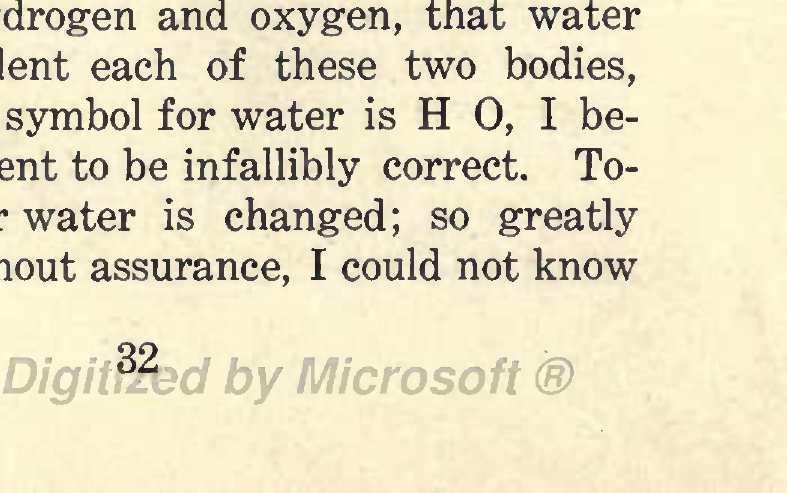
\includegraphics[width=0.8\textwidth]{../imagenes/pagina_040_fig_02.png}
\caption{Figura de la página 40}
\end{figure}

\begin{figure}[h!]
\centering
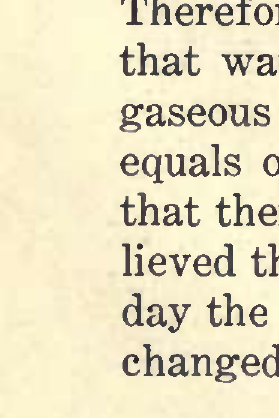
\includegraphics[width=0.8\textwidth]{../imagenes/pagina_040_fig_03.png}
\caption{Figura de la página 40}
\end{figure}

\begin{figure}[h!]
\centering
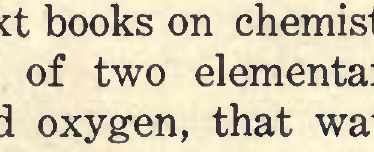
\includegraphics[width=0.8\textwidth]{../imagenes/pagina_040_fig_04.png}
\caption{Figura de la página 40}
\end{figure}

\begin{figure}[h!]
\centering
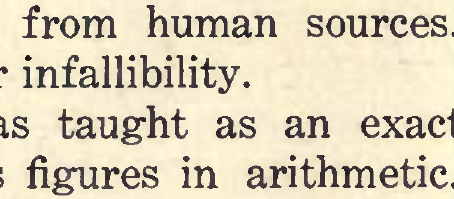
\includegraphics[width=0.8\textwidth]{../imagenes/pagina_040_fig_05.png}
\caption{Figura de la página 40}
\end{figure}

\begin{figure}[h!]
\centering
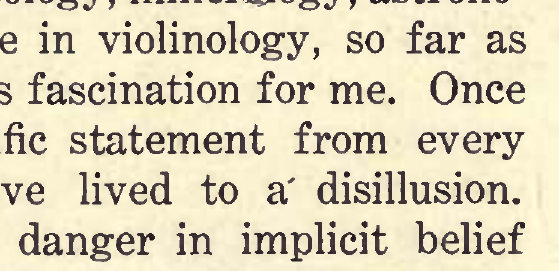
\includegraphics[width=0.8\textwidth]{../imagenes/pagina_040_fig_06.png}
\caption{Figura de la página 40}
\end{figure}

\begin{figure}[h!]
\centering
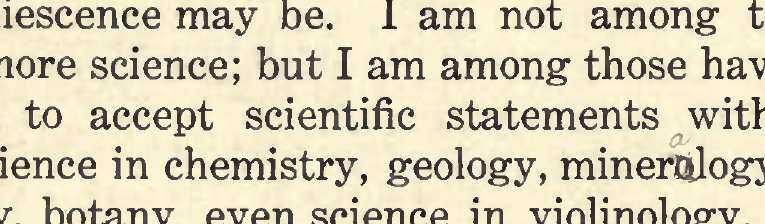
\includegraphics[width=0.8\textwidth]{../imagenes/pagina_040_fig_07.png}
\caption{Figura de la página 40}
\end{figure}

\begin{figure}[h!]
\centering
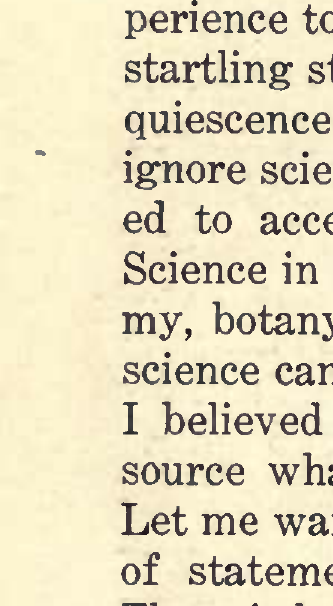
\includegraphics[width=0.8\textwidth]{../imagenes/pagina_040_fig_08.png}
\caption{Figura de la página 40}
\end{figure}

\begin{figure}[h!]
\centering
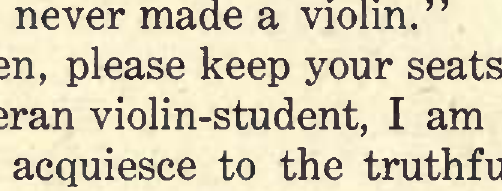
\includegraphics[width=0.8\textwidth]{../imagenes/pagina_040_fig_09.png}
\caption{Figura de la página 40}
\end{figure}

\begin{figure}[h!]
\centering
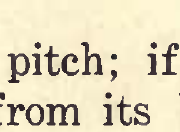
\includegraphics[width=0.8\textwidth]{../imagenes/pagina_040_fig_10.png}
\caption{Figura de la página 40}
\end{figure}

\begin{figure}[h!]
\centering
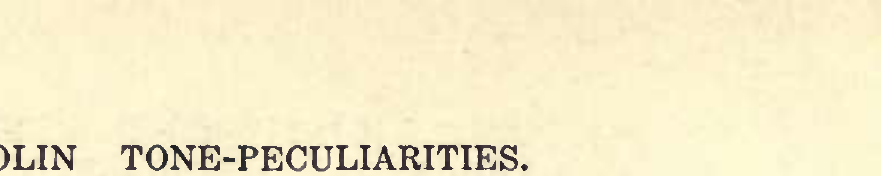
\includegraphics[width=0.8\textwidth]{../imagenes/pagina_040_fig_11.png}
\caption{Figura de la página 40}
\end{figure}

\section{VIOLIN TONE-PECULIARITIES.}

its free end, perceptibly raises its pitch; if too high, removal of only enough metal from its base to brighten the surface, lowers its pitch. I now believe a carefully graduated violin sound- ing-board to be equally as sensitive as either piano- wire, organ-reed, organ-pipe, or tuning-fork. "Science never made a violin." Gentlemen, please keep your seats. As a veteran violin-student, I am forced by ex- perience to acquiesce to the truthfullness in this startling statement, no matter how distasteful ac- quiescence may be. I am not among those who ignore science; but I am among those having learn- ed to accept scientific statements with caution. Science in chemistry, geology, mineralogy, astrono- my, botany, even science in violinology, so far as science can go, possesses fascination for me. Once I believed every scientific statement from every source whatever. I have lived to a' disillusion. Let me warn you of the danger in implicit belief of statements originating from human sources. There is but One Source for infallibility. In my day, chemistry was taught as an exact science, equally as exact as figures in arithmetic. Therefore, when I read in text books on chemistry that water is a combination of two elementary, gaseous bodies, hydrogen and oxygen, that water equals one equivalent each of these two bodies, that therefore the symbol for water is H 0, I be- lieved that statement to be infallibly correct. To- day the symbol for water is changed; so greatly changed that, without assurance, I could not know

32

\begin{figure}[h!]
\centering
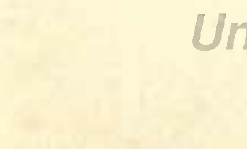
\includegraphics[width=0.8\textwidth]{../imagenes/pagina_041_fig_01.png}
\caption{Figura de la página 41}
\end{figure}

\begin{figure}[h!]
\centering

\includegraphics[width=0.8\textwidth]{../imagenes/pagina_041_fig_02.png}
\caption{Figura de la página 41}
\end{figure}

\begin{figure}[h!]
\centering

\includegraphics[width=0.8\textwidth]{../imagenes/pagina_041_fig_03.png}
\caption{Figura de la página 41}
\end{figure}

\begin{figure}[h!]
\centering
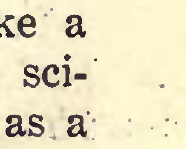
\includegraphics[width=0.8\textwidth]{../imagenes/pagina_041_fig_04.png}
\caption{Figura de la página 41}
\end{figure}

\begin{figure}[h!]
\centering
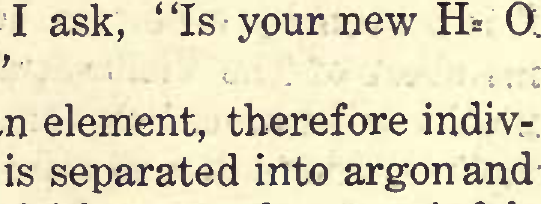
\includegraphics[width=0.8\textwidth]{../imagenes/pagina_041_fig_05.png}
\caption{Figura de la página 41}
\end{figure}

\begin{figure}[h!]
\centering
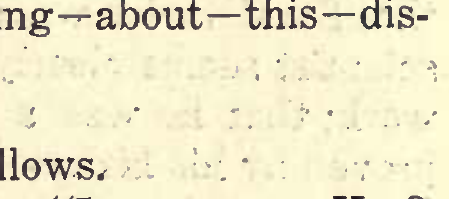
\includegraphics[width=0.8\textwidth]{../imagenes/pagina_041_fig_06.png}
\caption{Figura de la página 41}
\end{figure}

\section{VIOLIN TONE-PECULIARITIES.}

how H represents water. a Upon 1 a certain occasion at the University of Michigan, an incident occurred making an impres- sion on my mind to last until death. Twas at the hour for lecture on chemistry, wherein we were favored by the presence of an old gentleman who appeared deeply absorbed in. matter under discus- sion. Among other topics presented at this hour was distilled water, a gallon bottle of which . stood upon th6 lecturer's table. Instantly the lecture closed this attentive old gentlemen, with unsus- pected agility, climbed over railing to operating floor, pulled the cork from bottle of distilled water, applied his nose, shook his head,; shook the bottle, critically examined the "bead," then slowly in-- quired, "Is there T- any thing about this dis- tilled water intoxicating?"' Today I am the old man. You are the alert young fellows. In a subdued manner I ask, ' Is your new H= O. stronger than old HO?" Then, hydrogen was an element, therefore indiv- isible. Today hydrogen is separated into argon and boron. Pin not your faith upon human infal- libility; it is not in existence. Science is a Gollossus, yet, even today, science can't make a violin. Approaching the violin for its secrets, sci- ence, proud giant, receives a slap; on the face as a reminder that in the world there's one thing "none of his business. " In other directions, decade after decade, science advances with prodigious 'bounds; but in no scientific work can L find a solution for

33

\begin{figure}[h!]
\centering
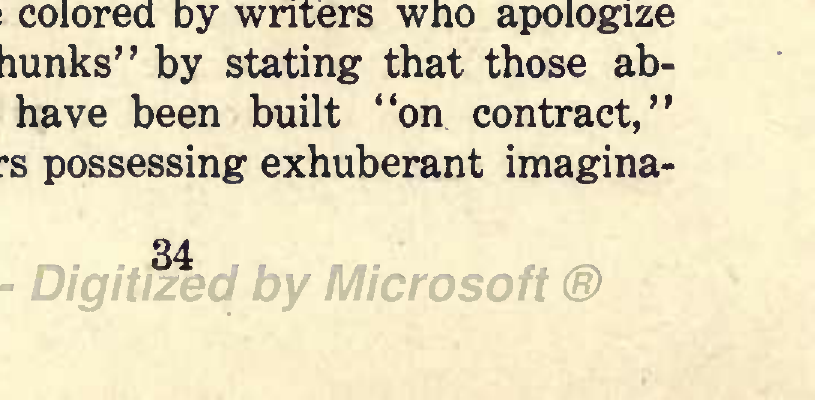
\includegraphics[width=0.8\textwidth]{../imagenes/pagina_042_fig_01.png}
\caption{Figura de la página 42}
\end{figure}

\begin{figure}[h!]
\centering
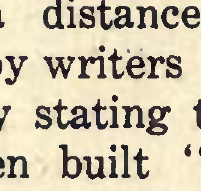
\includegraphics[width=0.8\textwidth]{../imagenes/pagina_042_fig_02.png}
\caption{Figura de la página 42}
\end{figure}

\begin{figure}[h!]
\centering
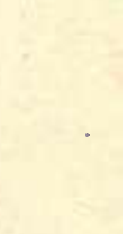
\includegraphics[width=0.8\textwidth]{../imagenes/pagina_042_fig_03.png}
\caption{Figura de la página 42}
\end{figure}

\begin{figure}[h!]
\centering
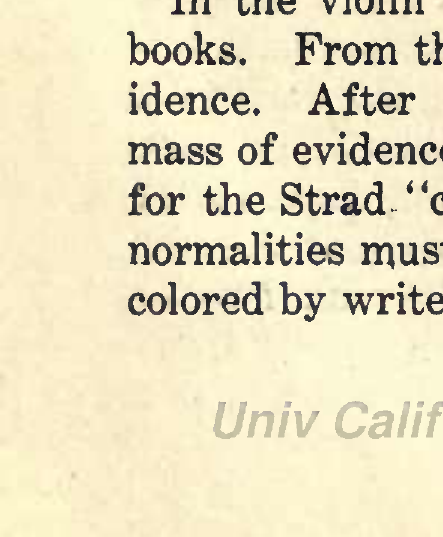
\includegraphics[width=0.8\textwidth]{../imagenes/pagina_042_fig_04.png}
\caption{Figura de la página 42}
\end{figure}

\begin{figure}[h!]
\centering
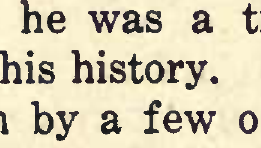
\includegraphics[width=0.8\textwidth]{../imagenes/pagina_042_fig_05.png}
\caption{Figura de la página 42}
\end{figure}

\begin{figure}[h!]
\centering
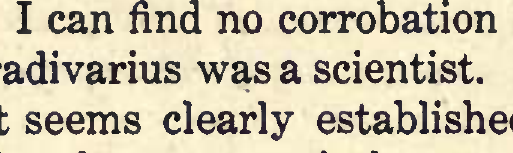
\includegraphics[width=0.8\textwidth]{../imagenes/pagina_042_fig_06.png}
\caption{Figura de la página 42}
\end{figure}

\begin{figure}[h!]
\centering
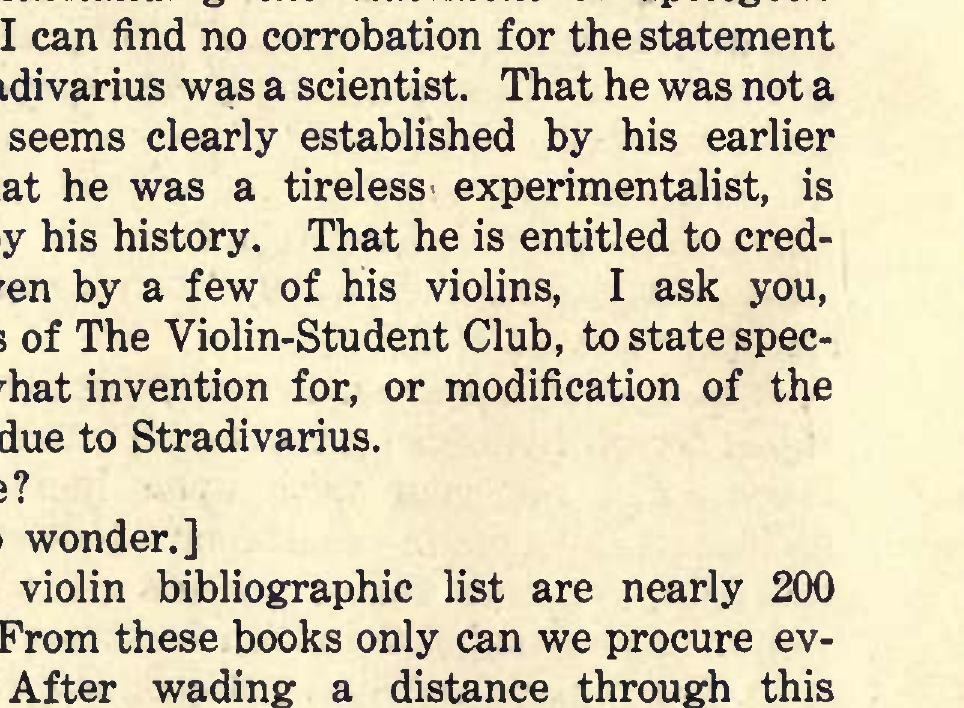
\includegraphics[width=0.8\textwidth]{../imagenes/pagina_042_fig_07.png}
\caption{Figura de la página 42}
\end{figure}

\begin{figure}[h!]
\centering
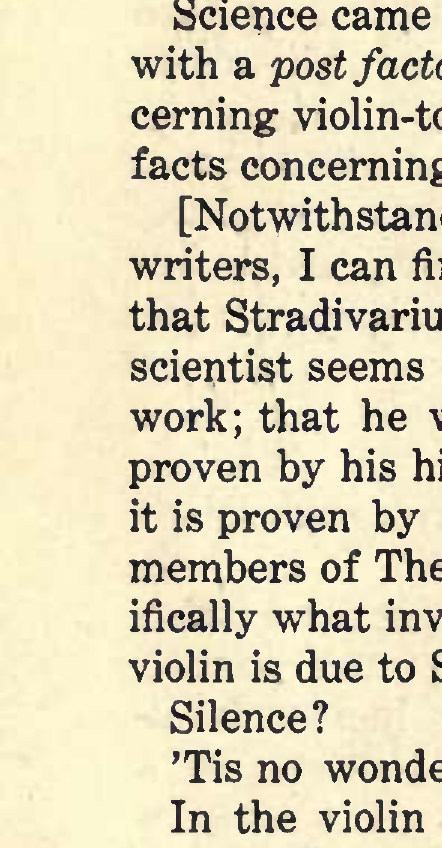
\includegraphics[width=0.8\textwidth]{../imagenes/pagina_042_fig_08.png}
\caption{Figura de la página 42}
\end{figure}

\begin{figure}[h!]
\centering
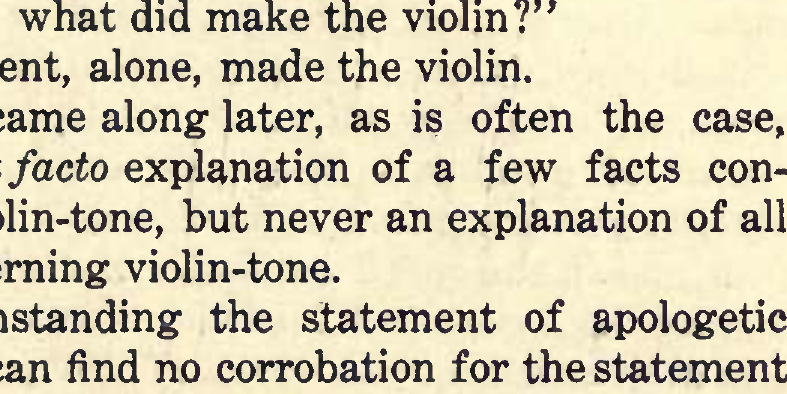
\includegraphics[width=0.8\textwidth]{../imagenes/pagina_042_fig_09.png}
\caption{Figura de la página 42}
\end{figure}

\begin{figure}[h!]
\centering

\includegraphics[width=0.8\textwidth]{../imagenes/pagina_042_fig_10.png}
\caption{Figura de la página 42}
\end{figure}

\begin{figure}[h!]
\centering
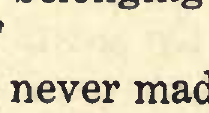
\includegraphics[width=0.8\textwidth]{../imagenes/pagina_042_fig_11.png}
\caption{Figura de la página 42}
\end{figure}

\begin{figure}[h!]
\centering
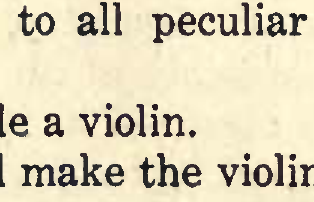
\includegraphics[width=0.8\textwidth]{../imagenes/pagina_042_fig_12.png}
\caption{Figura de la página 42}
\end{figure}

\begin{figure}[h!]
\centering
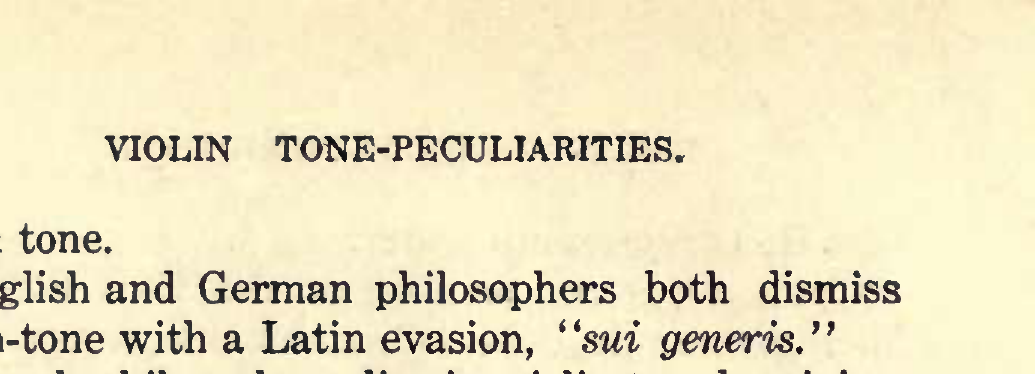
\includegraphics[width=0.8\textwidth]{../imagenes/pagina_042_fig_13.png}
\caption{Figura de la página 42}
\end{figure}

\section{VIOLIN TONE-PECULIARITIES.}

violin tone. English and German philosophers both dismiss violin-tone with a Latin evasion, "sui generis." French philosophers dismiss violin-tone by giving it a name belonging to all peculiar musical tone, "ft'w\&re." Science never made a violin. "Doctor, what did make the violin?" Experiment, alone, made the violin. Science came along later, as is often the case, with a post facto explanation of a few facts con- cerning violin-tone, but never an explanation of all facts concerning violin-tone. [Notwithstanding the statement of apologetic writers, I can find no corrobation for the statement that Stradivarius was a scientist. That he was not a scientist seems clearly established by his earlier work; that he was a tireless experimentalist, is proven by his history. That he is entitled to cred- it is proven by a few of his violins, I ask you, members of The Violin-Student Club, to state spec- ifically what invention for, or modification of the violin is due to Stradivarius. Silence? 'Tis no wonder.] In the violin bibliographic list are nearly 200 books. From these books only can we procure ev- idence. After wading a distance through this mass of evidence colored by writers who apologize for the Strad "chunks" by stating that those ab- normalities must have been built "on contract," colored by writers possessing exhuberant imagina-

34

\begin{figure}[h!]
\centering
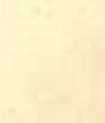
\includegraphics[width=0.8\textwidth]{../imagenes/pagina_043_fig_01.png}
\caption{Figura de la página 43}
\end{figure}

\begin{figure}[h!]
\centering
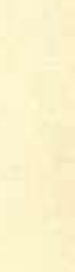
\includegraphics[width=0.8\textwidth]{../imagenes/pagina_043_fig_02.png}
\caption{Figura de la página 43}
\end{figure}

\begin{figure}[h!]
\centering
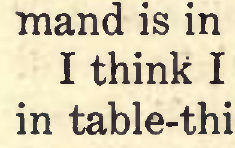
\includegraphics[width=0.8\textwidth]{../imagenes/pagina_043_fig_03.png}
\caption{Figura de la página 43}
\end{figure}

\begin{figure}[h!]
\centering
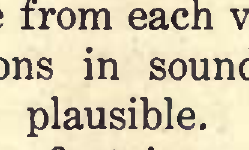
\includegraphics[width=0.8\textwidth]{../imagenes/pagina_043_fig_04.png}
\caption{Figura de la página 43}
\end{figure}

\begin{figure}[h!]
\centering
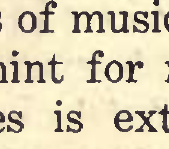
\includegraphics[width=0.8\textwidth]{../imagenes/pagina_043_fig_05.png}
\caption{Figura de la página 43}
\end{figure}

\begin{figure}[h!]
\centering
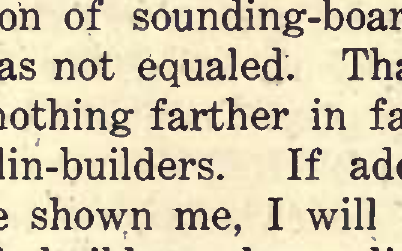
\includegraphics[width=0.8\textwidth]{../imagenes/pagina_043_fig_06.png}
\caption{Figura de la página 43}
\end{figure}

\begin{figure}[h!]
\centering
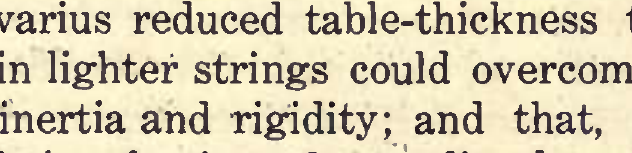
\includegraphics[width=0.8\textwidth]{../imagenes/pagina_043_fig_07.png}
\caption{Figura de la página 43}
\end{figure}

\begin{figure}[h!]
\centering
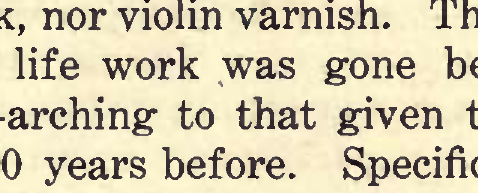
\includegraphics[width=0.8\textwidth]{../imagenes/pagina_043_fig_08.png}
\caption{Figura de la página 43}
\end{figure}

\begin{figure}[h!]
\centering
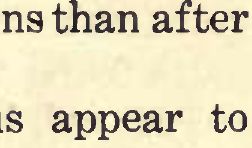
\includegraphics[width=0.8\textwidth]{../imagenes/pagina_043_fig_09.png}
\caption{Figura de la página 43}
\end{figure}

\begin{figure}[h!]
\centering
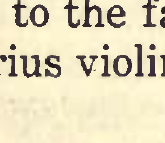
\includegraphics[width=0.8\textwidth]{../imagenes/pagina_043_fig_10.png}
\caption{Figura de la página 43}
\end{figure}

\begin{figure}[h!]
\centering
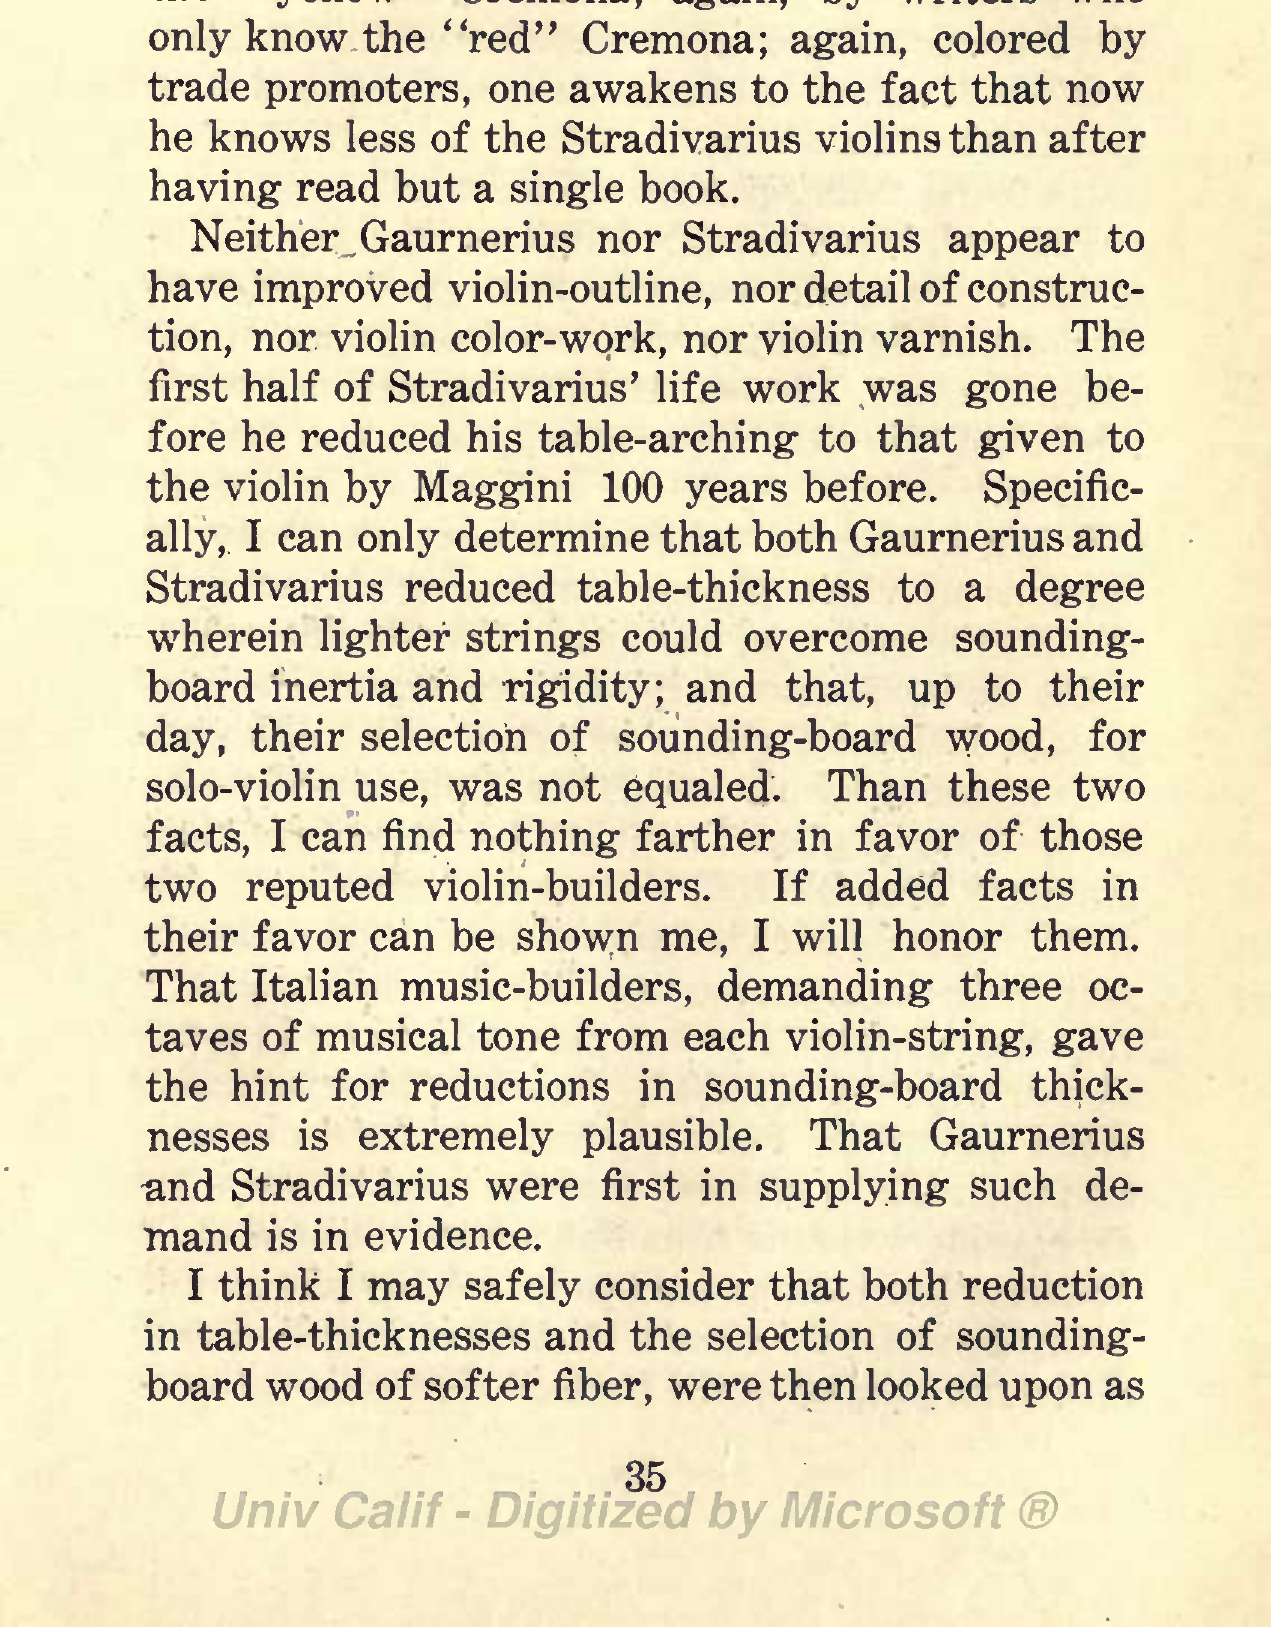
\includegraphics[width=0.8\textwidth]{../imagenes/pagina_043_fig_11.png}
\caption{Figura de la página 43}
\end{figure}

\begin{figure}[h!]
\centering
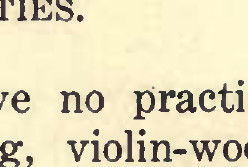
\includegraphics[width=0.8\textwidth]{../imagenes/pagina_043_fig_12.png}
\caption{Figura de la página 43}
\end{figure}

\begin{figure}[h!]
\centering
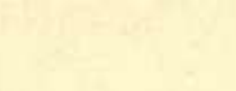
\includegraphics[width=0.8\textwidth]{../imagenes/pagina_043_fig_13.png}
\caption{Figura de la página 43}
\end{figure}

\begin{figure}[h!]
\centering
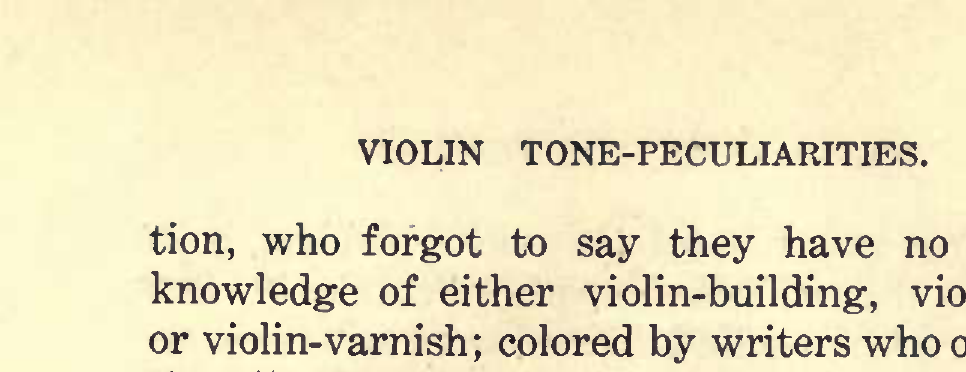
\includegraphics[width=0.8\textwidth]{../imagenes/pagina_043_fig_14.png}
\caption{Figura de la página 43}
\end{figure}

\section{VIOLIN TONE-PECULIARITIES.}

tion, who forgot to say they have no practical knowledge of either violin-building, violin-wood, or violin- varnish; colored by writers who only know the ' 'yellow" Cremona; again, by writers who only know the "red" Cremona; again, colored by trade promoters, one awakens to the fact that now he knows less of the Stradivarius violins than after having read but a single book. Neither. Gaurnerius nor Stradivarius appear to have improved violin-outline, nor detail of construc- tion, nor violin color- work, nor violin varnish. The first half of Stradivarius' life work was gone be- fore he reduced his table-arching to that given to the violin by Maggini 100 years before. Specific- ally, I can only determine that both Gaurnerius and Stradivarius reduced table-thickness to a degree wherein lighter strings could overcome sounding- board inertia and rigidity; and that, up to their day, their selection of sounding-board wood, for solo- violin use, was not equaled. Than these two facts, I can find nothing farther in favor of those two reputed violin-builders. If added facts in their favor can be shown me, I will honor them. That Italian music-builders, demanding three oc- taves of musical tone from each violin-string, gave the hint for reductions in sounding-board thick- nesses is extremely plausible. That Gaurnerius and Stradivarius were first in supplying such de- mand is in evidence. I think I may safely consider that both reduction in table-thicknesses and the selection of sounding- board wood of softer fiber, were then looked upon as

35

\begin{figure}[h!]
\centering

\includegraphics[width=0.8\textwidth]{../imagenes/pagina_044_fig_01.png}
\caption{Figura de la página 44}
\end{figure}

\begin{figure}[h!]
\centering
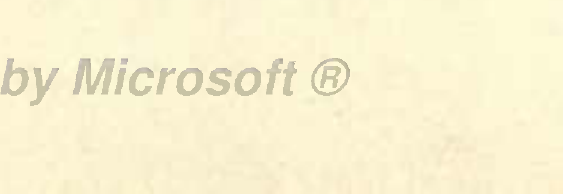
\includegraphics[width=0.8\textwidth]{../imagenes/pagina_044_fig_02.png}
\caption{Figura de la página 44}
\end{figure}

\begin{figure}[h!]
\centering
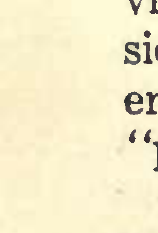
\includegraphics[width=0.8\textwidth]{../imagenes/pagina_044_fig_03.png}
\caption{Figura de la página 44}
\end{figure}

\begin{figure}[h!]
\centering

\includegraphics[width=0.8\textwidth]{../imagenes/pagina_044_fig_04.png}
\caption{Figura de la página 44}
\end{figure}

\begin{figure}[h!]
\centering
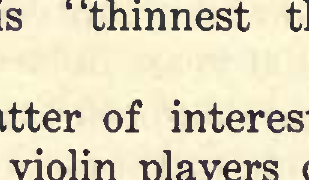
\includegraphics[width=0.8\textwidth]{../imagenes/pagina_044_fig_05.png}
\caption{Figura de la página 44}
\end{figure}

\begin{figure}[h!]
\centering
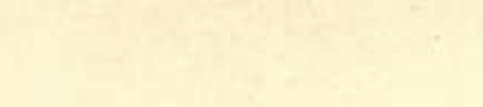
\includegraphics[width=0.8\textwidth]{../imagenes/pagina_044_fig_06.png}
\caption{Figura de la página 44}
\end{figure}

\section{VIOLIN TONE-PECULIARITIES.}

innovations; and that, by other violin-builders, both of these men were looked upon as "cranks." But both men, as solo-violin-builders, were winners, al- though each adopted a different plan for accom- plishing 1 sounding-board reductions of thicknesses. Ole Bull demanded four octaves of musical tone from each violin-string. He found satisfaction in a ' 'Joseph. ' ' Paganni, it is claimed, delighted in light violin- strings. Paganni was the first great soloist to exploit the Gaurnerius violin. Honeyman, in an indefinite way, states that the Gaurnerius sound- ing-board is "thinnest throughout the central portion. ' ' It is a matter of interest to note the varying opinions of violin players concerning the varying tone in the violins of the great violin-builders. Ole Bull expresses surprise at seeing his contem- porary, DeBeriot, appear in public with a Maggini. In speaking of his Strad, Ole Bull substantially says, "I never play it in public because of its nasal twang," (See Ole Bull Memoirs, by Sarah C., his wife. ) I call your attention to notable omission in statements concerning the Stradivarius violins that the speaker or writer generally omits to men- tion in which of Strad 's "periods" his particular violin was made. I can only account for such omis- sion upon the hypothesis that the speaker, or writ- er, considers violins from only one of Strad 's four "periods" to possess tone- value worthy of remark. Gentlemen, you make a mistake if you interpret me as not joining in the praise universally accord-

36

\begin{figure}[h!]
\centering
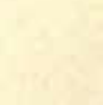
\includegraphics[width=0.8\textwidth]{../imagenes/pagina_045_fig_01.png}
\caption{Figura de la página 45}
\end{figure}

\begin{figure}[h!]
\centering
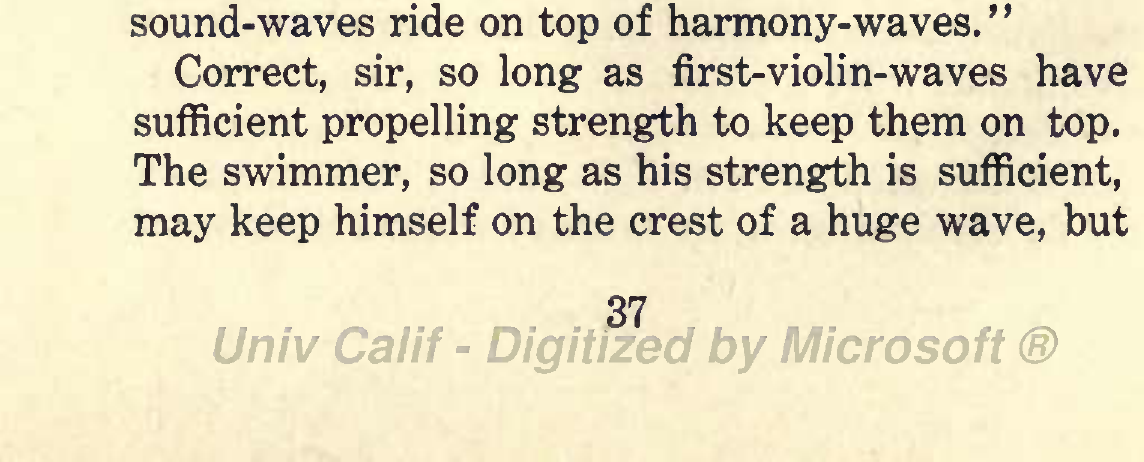
\includegraphics[width=0.8\textwidth]{../imagenes/pagina_045_fig_02.png}
\caption{Figura de la página 45}
\end{figure}

\begin{figure}[h!]
\centering
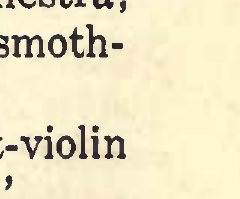
\includegraphics[width=0.8\textwidth]{../imagenes/pagina_045_fig_03.png}
\caption{Figura de la página 45}
\end{figure}

\begin{figure}[h!]
\centering
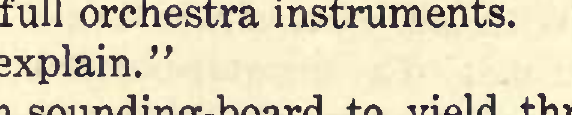
\includegraphics[width=0.8\textwidth]{../imagenes/pagina_045_fig_04.png}
\caption{Figura de la página 45}
\end{figure}

\begin{figure}[h!]
\centering
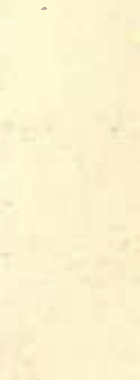
\includegraphics[width=0.8\textwidth]{../imagenes/pagina_045_fig_05.png}
\caption{Figura de la página 45}
\end{figure}

\begin{figure}[h!]
\centering
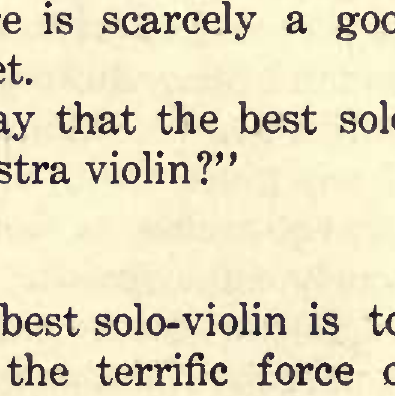
\includegraphics[width=0.8\textwidth]{../imagenes/pagina_045_fig_06.png}
\caption{Figura de la página 45}
\end{figure}

\begin{figure}[h!]
\centering
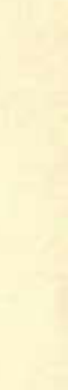
\includegraphics[width=0.8\textwidth]{../imagenes/pagina_045_fig_07.png}
\caption{Figura de la página 45}
\end{figure}

\begin{figure}[h!]
\centering
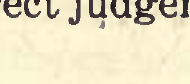
\includegraphics[width=0.8\textwidth]{../imagenes/pagina_045_fig_08.png}
\caption{Figura de la página 45}
\end{figure}

\begin{figure}[h!]
\centering
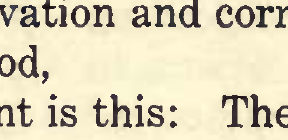
\includegraphics[width=0.8\textwidth]{../imagenes/pagina_045_fig_09.png}
\caption{Figura de la página 45}
\end{figure}

\begin{figure}[h!]
\centering
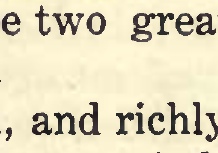
\includegraphics[width=0.8\textwidth]{../imagenes/pagina_045_fig_10.png}
\caption{Figura de la página 45}
\end{figure}

\begin{figure}[h!]
\centering
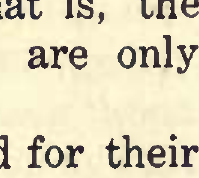
\includegraphics[width=0.8\textwidth]{../imagenes/pagina_045_fig_11.png}
\caption{Figura de la página 45}
\end{figure}

\begin{figure}[h!]
\centering
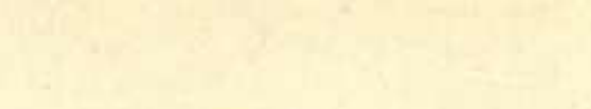
\includegraphics[width=0.8\textwidth]{../imagenes/pagina_045_fig_12.png}
\caption{Figura de la página 45}
\end{figure}

\begin{figure}[h!]
\centering
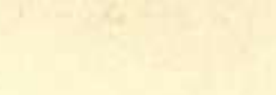
\includegraphics[width=0.8\textwidth]{../imagenes/pagina_045_fig_13.png}
\caption{Figura de la página 45}
\end{figure}

\section{VIOLIN TONE-PECULIARITIES.}

ed these two famous violin builders; but my praise is bestowed only for a definite reason that is, the great violins of these two great makers ; are only great as solo-violins. "Pis honor enough, and richly deserved for their bold innovation and correct judgement of sounding- board wood, My point is this: The unlimited praise bestowed upon these solo-violins has driven an army of vio- lin-makers to life-long effort at reproduction of solo-violins, until today, there is scarcely a good orchestra violin on the market. "Doctor, do you mean to say that the best solo- violin is not also a best orchestra violin?"

Yes, sir. "How is that?" The sounding-board of the best solo-violin is too light in wood to withstand the terrific force of sound-waves from full orchestra instruments. " "Doctor, please explain. Thus: The violin sounding-board to yield three octaves of agreeable tone upon each string, must be reduced in thickness to the point of weakness in presence of harmony- waves from full-orchestra; and because of such weakness, its tones are smoth- ered by overpowering harmony-instruments. "But, Doctor, we understood that first- violin sound-waves ride on top of harmony- waves. ' ' Correct, sir, so long as first-violin-waves have sufficient propelling strength to keep them on top. The swimmer, so long as his strength is sufficient, may keep himself on the crest of a huge wave, but

37

\begin{figure}[h!]
\centering
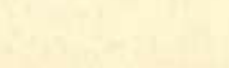
\includegraphics[width=0.8\textwidth]{../imagenes/pagina_046_fig_01.png}
\caption{Figura de la página 46}
\end{figure}

\begin{figure}[h!]
\centering
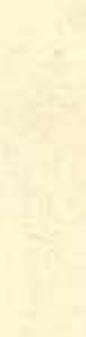
\includegraphics[width=0.8\textwidth]{../imagenes/pagina_046_fig_02.png}
\caption{Figura de la página 46}
\end{figure}

\begin{figure}[h!]
\centering
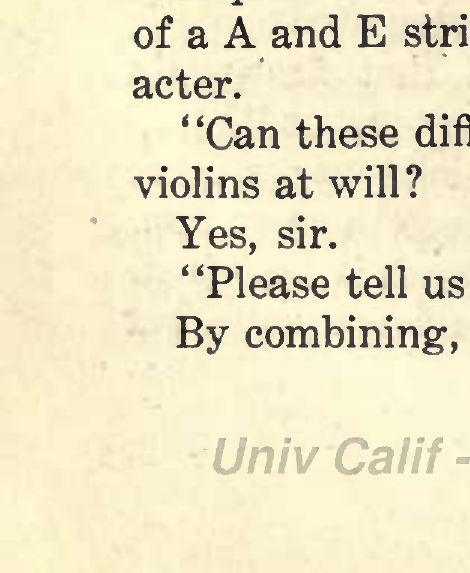
\includegraphics[width=0.8\textwidth]{../imagenes/pagina_046_fig_03.png}
\caption{Figura de la página 46}
\end{figure}

\begin{figure}[h!]
\centering
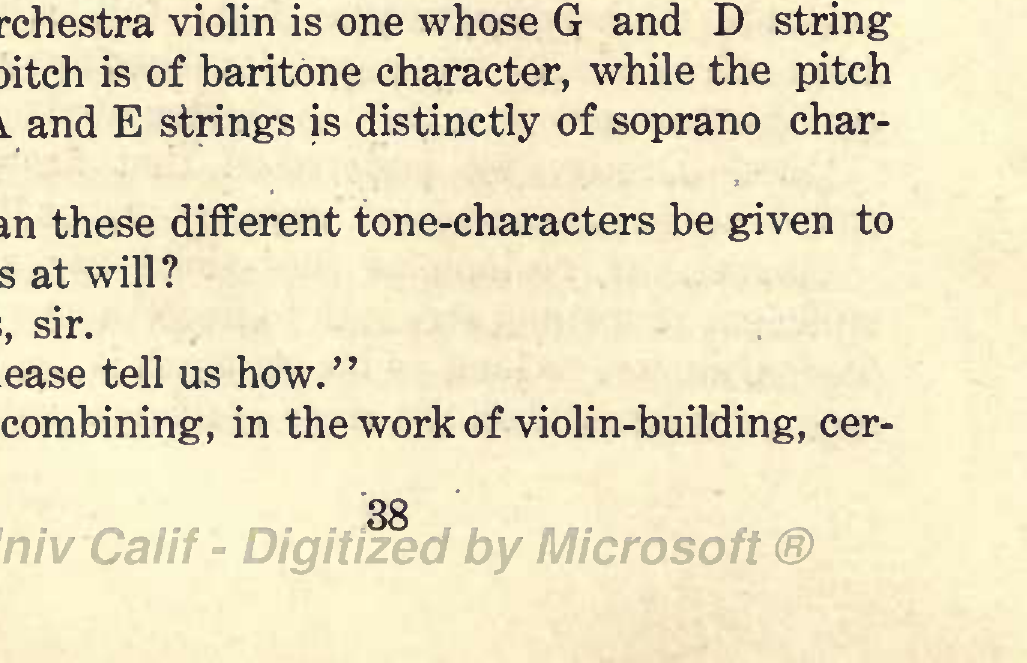
\includegraphics[width=0.8\textwidth]{../imagenes/pagina_046_fig_04.png}
\caption{Figura de la página 46}
\end{figure}

\begin{figure}[h!]
\centering
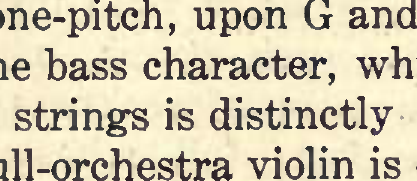
\includegraphics[width=0.8\textwidth]{../imagenes/pagina_046_fig_05.png}
\caption{Figura de la página 46}
\end{figure}

\begin{figure}[h!]
\centering
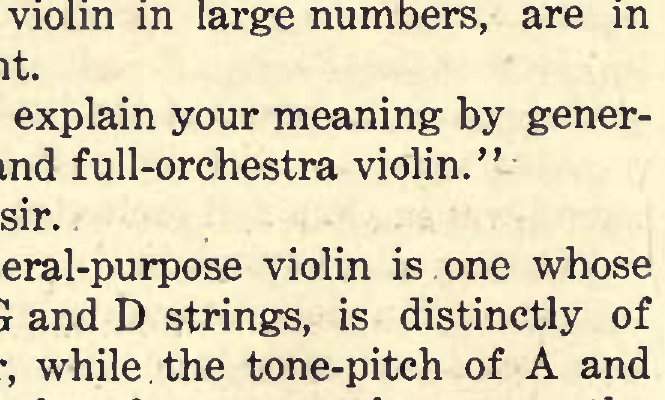
\includegraphics[width=0.8\textwidth]{../imagenes/pagina_046_fig_06.png}
\caption{Figura de la página 46}
\end{figure}

\begin{figure}[h!]
\centering
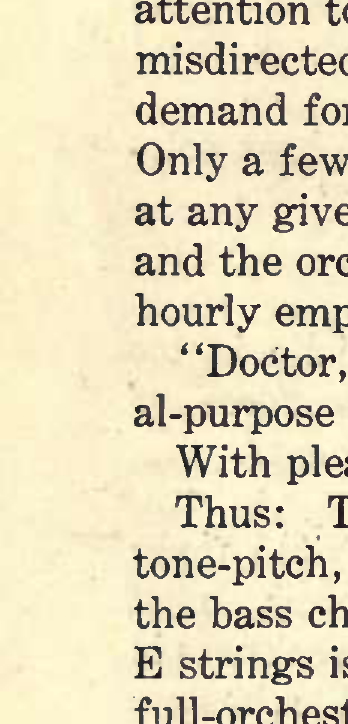
\includegraphics[width=0.8\textwidth]{../imagenes/pagina_046_fig_07.png}
\caption{Figura de la página 46}
\end{figure}

\begin{figure}[h!]
\centering
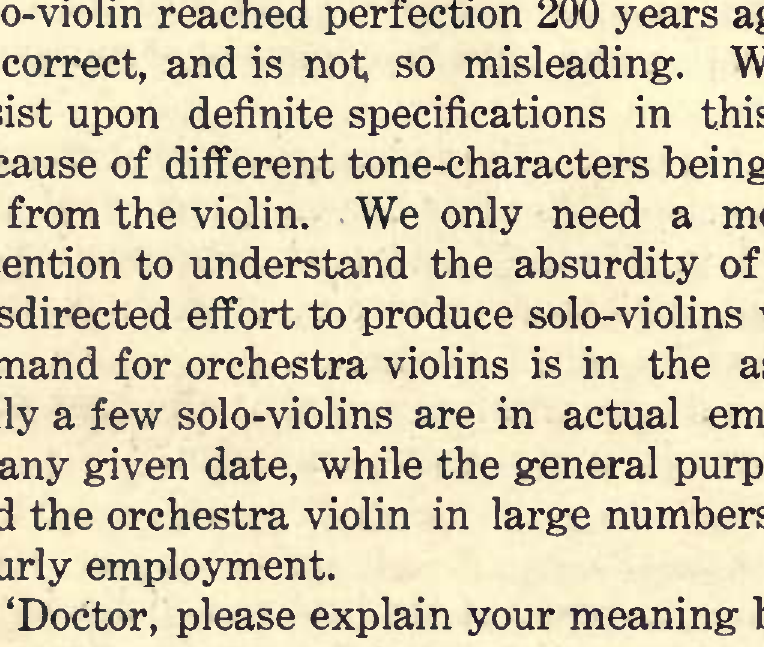
\includegraphics[width=0.8\textwidth]{../imagenes/pagina_046_fig_08.png}
\caption{Figura de la página 46}
\end{figure}

\begin{figure}[h!]
\centering
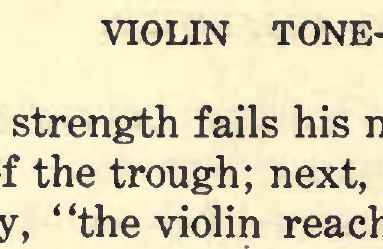
\includegraphics[width=0.8\textwidth]{../imagenes/pagina_046_fig_09.png}
\caption{Figura de la página 46}
\end{figure}

\begin{figure}[h!]
\centering
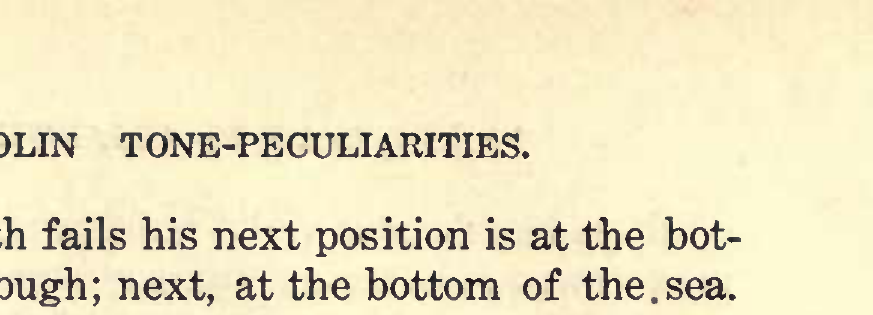
\includegraphics[width=0.8\textwidth]{../imagenes/pagina_046_fig_10.png}
\caption{Figura de la página 46}
\end{figure}

\section{VIOLIN TONE-PECULIARITIES.}

when strength fails his next position is at the bot- tom of the trough; next, at the bottom of the. sea. To say, ' 'the violin reached perfection 200 years ago," means much and means little. To say the solo- violin reached perfection 200 years ago is near- er correct, and is not so misleading. We should insist upon definite specifications in this matter, because of different tone-characters being demand- ed from the violin. We only need a moment of attention to understand the absurdity of so much misdirected effort to produce solo-violins while the demand for orchestra violins is in the ascendant. Only a few solo-violins are in actual employment at any given date, while the general purpose-violin and the orchestra violin in large numbers, are in hourly employment. "Doctor, please explain your meaning by gener- al-purpose violin and full-orchestra violin." With pleasure, sir. Thus: The general-purpose violin is one whose tone-pitch, upon G and D strings, is distinctly of the bass character, while the tone-pitch of A and E strings is distinctly of soprano character: the full-orchestra violin is one whose G and D string tone-pitch is of baritone character, while the pitch of a A and E strings is distinctly of soprano char- acter. "Can these different tone-characters be given to violins at will?

Yes, sir. "Please tell us how." By combining, in the work of violin-building, cer-

38

\begin{figure}[h!]
\centering

\includegraphics[width=0.8\textwidth]{../imagenes/pagina_047_fig_01.png}
\caption{Figura de la página 47}
\end{figure}

\begin{figure}[h!]
\centering

\includegraphics[width=0.8\textwidth]{../imagenes/pagina_047_fig_02.png}
\caption{Figura de la página 47}
\end{figure}

\section{VIOLIN TONE-PECULIARITIES.}

tain rules to be found in Lecture III, governing pitch of tone-producing agents. By reason of repeated, practical demonstrations, I am able to assure correctness of these rules. Before leaving the question of ' Violin perfection 200 years ago," let me direct your attention to two of its evil consequences. First: It acts as a discouragement to further experiment. Second: It acts to place a fictitious value upon a few violins of that date. Industrious "trade promoters" have lost no op- portunity for befogging the public in the matter of old, solo- violin values; thus the public erroneously demands that every soloist shall appear only with either a ' 'Joseph* ' or a ' 'Strad' ' under his arm. But, today there are unmistakable signs that the public is emerging from the fog; a few observing persons, having the courage of conviction, pronounce "pass- ing benediction" upon the "old violin." My own veneration, reverance, worship, call it what you will, for the "old violin" was cruelly shattered years ago by discovering that the violin may be- come "too old", also, by discovering the fact that a modern violin can be made to appear ' 'remark- ably preserved." But a few years ago the public was given an op- portunity for observing the inanity of continuing the demand that the soloist use only old violins upon all occasions. 'Twas at the Chicago Auditorium. My friend, Mr. Beebe, himself a violin-maker of repute, upon first occasion, seated himself quite

39

\begin{figure}[h!]
\centering
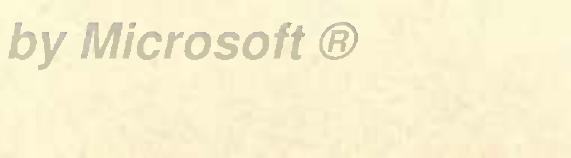
\includegraphics[width=0.8\textwidth]{../imagenes/pagina_048_fig_01.png}
\caption{Figura de la página 48}
\end{figure}

\begin{figure}[h!]
\centering

\includegraphics[width=0.8\textwidth]{../imagenes/pagina_048_fig_02.png}
\caption{Figura de la página 48}
\end{figure}

\begin{figure}[h!]
\centering
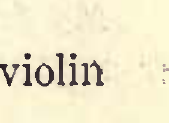
\includegraphics[width=0.8\textwidth]{../imagenes/pagina_048_fig_03.png}
\caption{Figura de la página 48}
\end{figure}

\begin{figure}[h!]
\centering
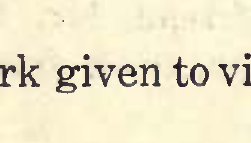
\includegraphics[width=0.8\textwidth]{../imagenes/pagina_048_fig_04.png}
\caption{Figura de la página 48}
\end{figure}

\begin{figure}[h!]
\centering
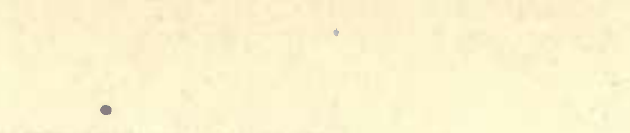
\includegraphics[width=0.8\textwidth]{../imagenes/pagina_048_fig_05.png}
\caption{Figura de la página 48}
\end{figure}

\section{VIOLIN TONE-PECULIARITIES.'}

near the stage; upon a second occasion, seated him- self farther away from the stage; and, upon a third occasion, in the most distant seat; all for the pur- pose of judging tone from a Strad in the hands of a star soloist wise enough to permit only piano ac* companiment for his old violin. Mr. Beebe rejoices in scheduling a musically-trained ear, and I, of my own knowledge, have assurance that said ear, in the presence of violin tone, stands conspicuously forward. 'Therefore, when Mr. Beebe states that, while in a distant Auditorium seat, certain efforts of the great violinist were disappointing because of weakness in the tone of that old violin, I accept such statement as coming from a reliable authority. This incident shows the fictitious value placed upon old violins. That Strad is valued at several thousands a Beebe at a few hundreds. I value most that violin having the most satisfying tone. Gentlemen: Let me advise that you build violins with a view to some particular place of usefullness. Thus, when building for solo use, reduce sounding- board thickness to a degree yielding three octaves of musical sound from each string. When building a general-purpose violin, reduce dimensions of bar and sounding-board beneath >G and D strings to give those strings the basso tone-character, while leaving sufficient wood beneath A and E strings to give thein the soprano tone-pitch. In building for orchestra us\textasciicircum\{\}e, then leave sufficient wood beneath all strings to secure the baritone-soprano tone- character. ' < ' After fifty years of practical work given to violin

40

\begin{figure}[h!]
\centering
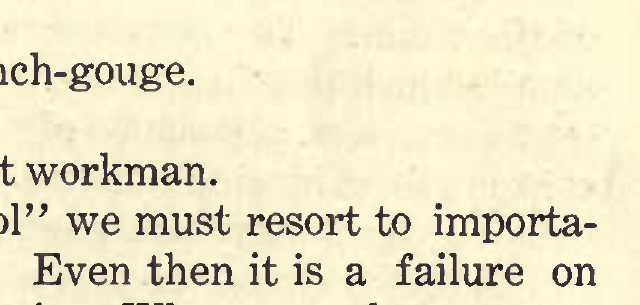
\includegraphics[width=0.8\textwidth]{../imagenes/pagina_049_fig_01.png}
\caption{Figura de la página 49}
\end{figure}

\begin{figure}[h!]
\centering
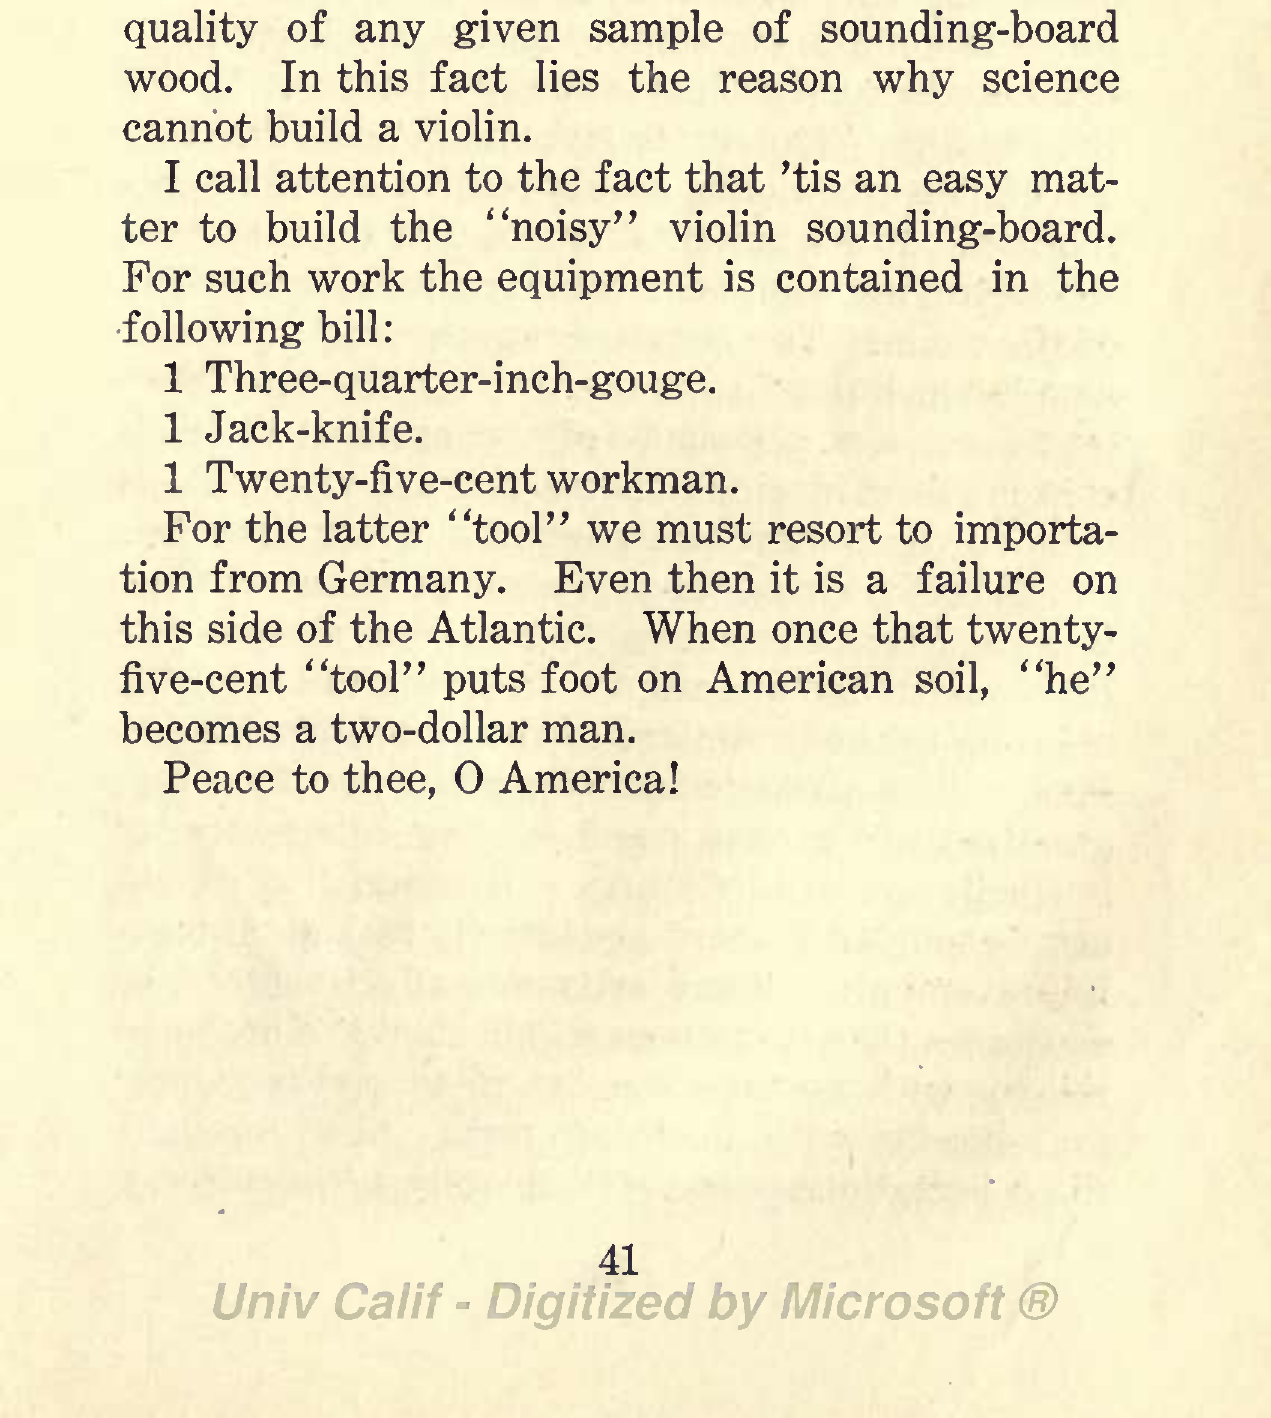
\includegraphics[width=0.8\textwidth]{../imagenes/pagina_049_fig_02.png}
\caption{Figura de la página 49}
\end{figure}

\begin{figure}[h!]
\centering
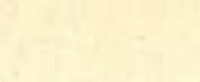
\includegraphics[width=0.8\textwidth]{../imagenes/pagina_049_fig_03.png}
\caption{Figura de la página 49}
\end{figure}

\begin{figure}[h!]
\centering
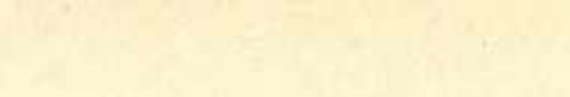
\includegraphics[width=0.8\textwidth]{../imagenes/pagina_049_fig_04.png}
\caption{Figura de la página 49}
\end{figure}

VIOLIN TONE-PECULIARITIES. tone-peculiarities, such are my conclusions in the matter of violin building. I call your attention to the fact that, in skillfully made violins, a wide range of tone- value exists; and to the fact that such wide range of tone- value is due to inherent differences in quality of sounding- board wood. Neither you, nor I, nor any person whatsoever, can exactly pre-determine the tone- quality of any given sample of sounding-board wood. In this fact lies the reason why science cannot build a violin. I call attention to the fact that 'tis an easy mat- ter to build the "noisy" violin sounding-board. For such work the equipment is contained in the following bill: 1 Three-quarter-inch-gouge. 1 Jack-knife. 1 Twenty-five-cent workman. For the latter "tool" we must resort to importa- tion from Germany. Even then it is a failure on this side of the Atlantic. When once that twenty- five-cent "tool" puts foot on American soil, "he" becomes a two-dollar man. Peace to thee, America!

41

\begin{figure}[h!]
\centering

\includegraphics[width=0.8\textwidth]{../imagenes/pagina_050_fig_01.png}
\caption{Figura de la página 50}
\end{figure}

\begin{figure}[h!]
\centering

\includegraphics[width=0.8\textwidth]{../imagenes/pagina_050_fig_02.png}
\caption{Figura de la página 50}
\end{figure}

\begin{figure}[h!]
\centering
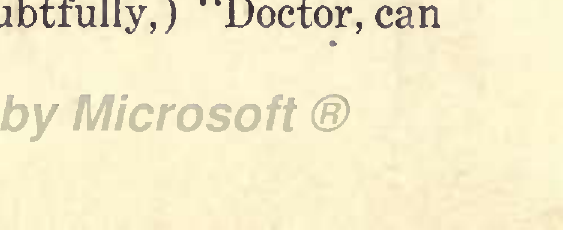
\includegraphics[width=0.8\textwidth]{../imagenes/pagina_050_fig_03.png}
\caption{Figura de la página 50}
\end{figure}

\begin{figure}[h!]
\centering
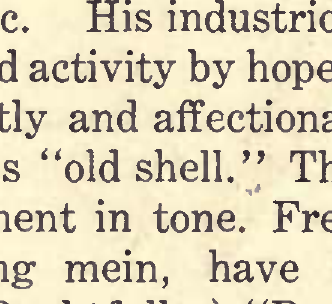
\includegraphics[width=0.8\textwidth]{../imagenes/pagina_050_fig_04.png}
\caption{Figura de la página 50}
\end{figure}

\begin{figure}[h!]
\centering
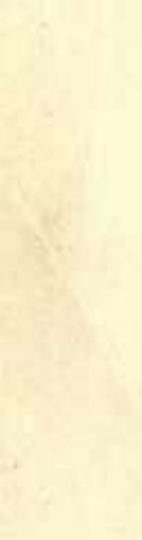
\includegraphics[width=0.8\textwidth]{../imagenes/pagina_050_fig_05.png}
\caption{Figura de la página 50}
\end{figure}

\begin{figure}[h!]
\centering
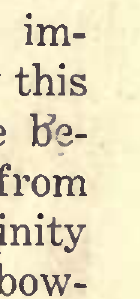
\includegraphics[width=0.8\textwidth]{../imagenes/pagina_050_fig_06.png}
\caption{Figura de la página 50}
\end{figure}

\begin{figure}[h!]
\centering
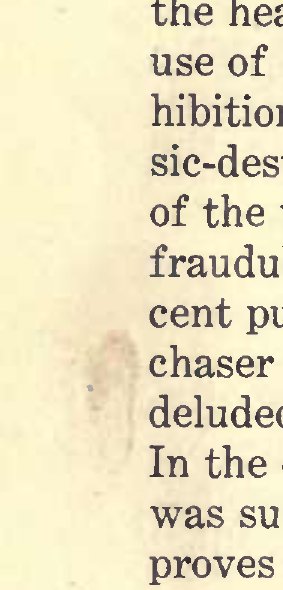
\includegraphics[width=0.8\textwidth]{../imagenes/pagina_050_fig_07.png}
\caption{Figura de la página 50}
\end{figure}

\begin{figure}[h!]
\centering
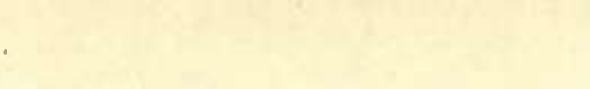
\includegraphics[width=0.8\textwidth]{../imagenes/pagina_050_fig_08.png}
\caption{Figura de la página 50}
\end{figure}

\section{VIOLIN TONE-PECULIARITIES.}

LECTURE III. GENTLEMEN: You understand the aim of our society includes the study of both musical and un- musical sound produced by the violin. It is not agreeable to admit other than musical tone as a pos- sibility for the violin. Instinctively, we are wont to consider "sweetness" and "violin" to be synon- ymous terms. Even to speak of the "noisy" vio- lin, is rasping to our sensory nerves, while enforced listening to such violins is positive torture. Under the heading, "Cruelty to Humanity," the sale and use of "noisy" violins should receive statutory pro- hibition. It is a lamentable fact that the most mu- sic-destroying sound can come from close imitations of the violin. The outward appearance of these fraudulent imitations is the trap set for the inno- cent purchaser. Because of appearances, the pur- chaser thinks himself in possession of a violin. Such deluded victims are today found in every direction. In the credulous ear of every one of these victims was sung that siren song, ' 'The violin always im- proves with age and use." In trying to apply this old song to the imitations of the violin, trouble be- gins. The victim's family is made to suffer from an attack of "nerves," and, .his immediate vicinity is wholly avoided by Music. His industrious"bow- arm is spurred to increased activity by hope of tone- improvement. Steadfastly and affectionately, he addresses that imitation as "old shell." The years roll by with no improvement in tone. Frequently gray-heads, with doubting mein, have brought these imitations to me. (Doubtfully,) "Doctor, can

42

\begin{figure}[h!]
\centering
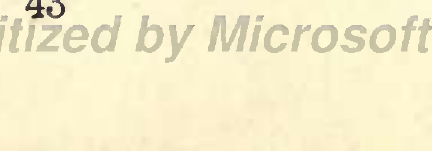
\includegraphics[width=0.8\textwidth]{../imagenes/pagina_051_fig_01.png}
\caption{Figura de la página 51}
\end{figure}

\begin{figure}[h!]
\centering
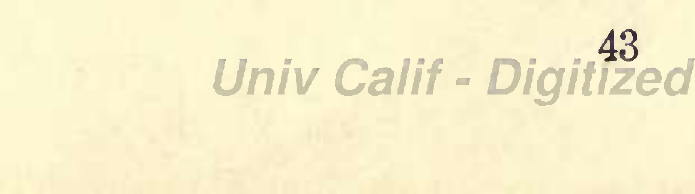
\includegraphics[width=0.8\textwidth]{../imagenes/pagina_051_fig_02.png}
\caption{Figura de la página 51}
\end{figure}

\begin{figure}[h!]
\centering
\includegraphics[width=0.8\textwidth]{../imagenes/pagina_051_fig_03.png}
\caption{Figura de la página 51}
\end{figure}

\begin{figure}[h!]
\centering
\includegraphics[width=0.8\textwidth]{../imagenes/pagina_051_fig_04.png}
\caption{Figura de la página 51}
\end{figure}

\begin{figure}[h!]
\centering
\includegraphics[width=0.8\textwidth]{../imagenes/pagina_051_fig_05.png}
\caption{Figura de la página 51}
\end{figure}

\section{VIOLIN TONE-PECULIARITIES.}

you tell me what ails my old shell?" Rapidly I run the bent "sound" across the inner surface of the sounding-board, the rattle therefrom suggesting the tinner's cart on corduroy road. "Yes, sir, I can tell you." "What is it?" "It's fraud." As I remove the sounding-board, permitting his doubt-expressing eyes to look upon the scene with- in his "old shell," the frozen smile on his wrinkled face is something truly pathetic. The graduation, (begging pardon for the use of that word, ) of this imitation sounding-board is entirely accomplished with gouge and jack-knife. The bar is a "chunk" left by haste of gouge, and thoughtfully smoothed by jack-knife upon the side exposed to your inspec- tion. Because you cannot see them, the two upper corners are forgotten. The linings, of various di- mensions, are both too long, and too short. Out- wardly, this fraud appears like the violin. Although the varnish is of cheap quality, the coloring is quite artistic. Here is a lifetime devoted to music, yet, wasted, wasted by this damnable imposition upon an inno- cent, credulous, unwary purchaser. Moreover, in this great, enlightened, (beg pardon once more, ) liberty-giving United States of North America, this same premeditated, unmitigated fraud is sold by thousands. Such gigantic imposition upon music- loving people is sufficient cause for murderous sen- timents within a heart of stone. These frauds are the product of combined cupidity, stupidity, and heart-

43

\begin{figure}[h!]
\centering
\includegraphics[width=0.8\textwidth]{../imagenes/pagina_052_fig_01.png}
\caption{Figura de la página 52}
\end{figure}

\begin{figure}[h!]
\centering
\includegraphics[width=0.8\textwidth]{../imagenes/pagina_052_fig_02.png}
\caption{Figura de la página 52}
\end{figure}

\begin{figure}[h!]
\centering
\includegraphics[width=0.8\textwidth]{../imagenes/pagina_052_fig_03.png}
\caption{Figura de la página 52}
\end{figure}

\begin{figure}[h!]
\centering
\includegraphics[width=0.8\textwidth]{../imagenes/pagina_052_fig_04.png}
\caption{Figura de la página 52}
\end{figure}

\begin{table}[h!]
\centering
\begin{tabular}{|l|}
\hline
VIOLIN TONE-PECULIARITIES. \\
\hline
lessness. Cupidity, in these frauds, is shown by charging more than kindling-wood prices, notwith- standing the fact that quotations are placed in the "pfennige" column. In these frauds, stupidity is shown in the fact that fifteen minutes more work upon the sounding-board might place quotations in the "marks" column. In these frauds, heartless- ness is shown by the premeditated murder of Music. The criminality of these fraud-builders ex- ceeds the criminality of one who robs little child- ren, because they combine murder with robbery. Poor Music! Standing aghast at sight of her fav- orite haunt no longer habitable! While professing friendship, you, Mr. Fraud-builder are the cause of her anguish. To you, and to such as you, and of you, I say ' 'Hell knoweth not a greater villain. ' ' \\
\hline
Thou Violin! Thou Who art sweet Music s only King! Must thy witching form conceal Cupidity's rankling deadly sting? Men! Arise! Stand up now In ranks of those who wish to fight To kill this robbing deadly thing, And give to Music hers by right. \\
\hline
"Doctor, how may the innocent purchaser know Cupidity's hand?" My friend, the case is hopeless when the purchas- er is so innocent as to be thereby unable to read, 'Made ' in Germany. ' ' After a lifetime given to the production of violin- \\
\hline
\end{tabular}
\end{table}

lessness. Cupidity, in these frauds, is shown by charging more than kindling-wood prices, notwith- standing the fact that quotations are placed in the "pfennige" column. In these frauds, stupidity is shown in the fact that fifteen minutes more work upon the sounding-board might place quotations in the "marks" column. In these frauds, heartless- ness is shown by the premeditated murder of Music. The criminality of these fraud-builders ex- ceeds the criminality of one who robs little child- ren, because they combine murder with robbery. Poor Music! Standing aghast at sight of her fav- orite haunt no longer habitable! While professing friendship, you, Mr. Fraud-builder are the cause of her anguish. To you, and to such as you, and of you, I say ' 'Hell knoweth not a greater villain. ' '

Thou Violin! Thou Who art sweet Music s only King! Must thy witching form conceal Cupidity's rankling deadly sting? Men! Arise! Stand up now In ranks of those who wish to fight To kill this robbing deadly thing, And give to Music hers by right.

"Doctor, how may the innocent purchaser know Cupidity's hand?" My friend, the case is hopeless when the purchas- er is so innocent as to be thereby unable to read, 'Made ' in Germany. ' ' After a lifetime given to the production of violin-

44

\begin{figure}[h!]
\centering
\includegraphics[width=0.8\textwidth]{../imagenes/pagina_053_fig_01.png}
\caption{Figura de la página 53}
\end{figure}

\begin{figure}[h!]
\centering
\includegraphics[width=0.8\textwidth]{../imagenes/pagina_053_fig_02.png}
\caption{Figura de la página 53}
\end{figure}

\section{VIOLIN TONE-PECULIARITIES.}

tone, I am compelled to acknowledge the disbelief in the possibility of satisfactory solution for all problems involved therein. I am also compelled to state that my experience, and conclusions, in the matter of how the violin operates to produce musi- cal sound, do not add corrobation to the theories of Savart, Honeyman, et al. Although unable to solve all problems in violin tone, yet, I do not re- gard my efforts thereat to be entirely fruitless. I give you my conclusions and principles, so far as they are satisfying to myself, in terms as clear in meaning and as concise in form as I am able to command. I shall not indulge in abstract theories. My conclusions are all worded after actual, practi- cal, repeated tests upon the used violin, except the principles of sounding-board graduation for maxi- mum evenness of tone. As will be shown later, this principle, for reasons of physical disability, re- ceived but a single demonstration. Whatever of value may exist in my conclusions is hereby be- queathed to you. I now call up the matter of violin tone-pitch. [This feature of violin tone is worthy of careful consideration. Other things being satisfactory, tone-pitch should govern the place of usefullness for each violin. Thus: The violin of low tone-pitch throughout should not be placed at the head of full orchestra, and, for the reason that its tones have not sufficient intensity, (carrying power) to satisfy the distant listening ear. The place for the violin of low tone-pitch throughout, is that of the solo instrument. Again, the violin of high tone-pitch

45

\begin{figure}[h!]
\centering
\includegraphics[width=0.8\textwidth]{../imagenes/pagina_054_fig_01.png}
\caption{Figura de la página 54}
\end{figure}

\begin{figure}[h!]
\centering
\includegraphics[width=0.8\textwidth]{../imagenes/pagina_054_fig_02.png}
\caption{Figura de la página 54}
\end{figure}

\section{VIOLIN TONE-PECULIARITIES.}

throughout, should not be employed as a solo in- strument, and, because its high-pitched tones, alone, are disagreeable to the listening ear. I have known the reputation of a creditable soloist to be ruined by his employment of a good, high-pitched, orchestra violin as a solo instrument.] I have formulated eight rules, each of which is capable of modifying violin tone-pitch. For con- venience of reference these rules are numbered consecutively from I to VIII. As frequent refer- ence will be given to these rules, they are therefore placed in a group. Rule /.Lengthening a tone-producing agent, other dimensions remaining equal, lowers tone- pitch. Rule //.Shortening a tone-producing agent, other dimensions remaining equal, raises tone-pitch. Rule III. Increasing thickness of a tone-produc- ing agent, other dimensions remaining equal, raises tone-pitch. Rule IV. Diminishing thickness of a tone-pro- ducing agent, other dimensions remaining equal, lowers tone-pitch. Rule V. Lengthening confined perpendicular air columns, lowers tone-pitch. Rule VI. Shortening confined, perpendicular air columns, raises tone-pitch. Rule VII. Enlarging sounding-board exits, raises tone-pitch. Rule VIII. Reducing sounding-board exits, low- ers tone-pitch. In practical violin building, or in violin toning,

46

\begin{figure}[h!]
\centering
\includegraphics[width=0.8\textwidth]{../imagenes/pagina_055_fig_01.png}
\caption{Figura de la página 55}
\end{figure}

\begin{figure}[h!]
\centering
\includegraphics[width=0.8\textwidth]{../imagenes/pagina_055_fig_02.png}
\caption{Figura de la página 55}
\end{figure}

\begin{figure}[h!]
\centering
\includegraphics[width=0.8\textwidth]{../imagenes/pagina_055_fig_03.png}
\caption{Figura de la página 55}
\end{figure}

\begin{figure}[h!]
\centering
\includegraphics[width=0.8\textwidth]{../imagenes/pagina_055_fig_04.png}
\caption{Figura de la página 55}
\end{figure}

\begin{figure}[h!]
\centering
\includegraphics[width=0.8\textwidth]{../imagenes/pagina_055_fig_05.png}
\caption{Figura de la página 55}
\end{figure}

\begin{figure}[h!]
\centering
\includegraphics[width=0.8\textwidth]{../imagenes/pagina_055_fig_06.png}
\caption{Figura de la página 55}
\end{figure}

\section{VIOLIN TONE-PECULIARITIES.}

each of these rules possesses value. In my practice, application of these rules is given to the sounding- board alone. In no way do I apply any of these rules to the back plate. After long continued ex- periment, I am come to the conclusion that the chief function of the back is that of a reflecting medium. Therefore, I only demand of the back sufficient rigidity to withstand, without a tremor, the terrific charge of molecular wave-movement originating at the inner surface of the sounding- board; and, that its fiber be fine, and dense, and susceptible of high polish. Thus, when "fin- ished," the inner surface of the back presents a perfect reflecting surface. I do not say that the back cannot modify tone-pitch. On the con- trary, I state that the rigidity of the back may be reduced until the tone-pitch of the violin is lowered to a hollow, feeble, worthless degree. I have found many violins thus ruined; more thus ruined than by great reduction of sounding-board rigid- ity. Indeed, many violin builders attempt to reg- ulate tone-pitch by reducing rigidity of the back. In my experience with the long-distance test for intensity, (carrying power) of tone, this manner of regulating tone-pitch has proven itself seriously erroneous. The tone of every violin, thus regulat- ed, has fallen far behind in the distance record. Speaking for myself, regulation of tone-pitch by reduction of sounding-board rigidity, has proven itself to be the safer method. Therefore, these rules for governing tone-pitch are applied to the sounding-board.

47

\begin{figure}[h!]
\centering
\includegraphics[width=0.8\textwidth]{../imagenes/pagina_056_fig_01.png}
\caption{Figura de la página 56}
\end{figure}

\begin{figure}[h!]
\centering
\includegraphics[width=0.8\textwidth]{../imagenes/pagina_056_fig_02.png}
\caption{Figura de la página 56}
\end{figure}

\begin{figure}[h!]
\centering
\includegraphics[width=0.8\textwidth]{../imagenes/pagina_056_fig_03.png}
\caption{Figura de la página 56}
\end{figure}

\begin{figure}[h!]
\centering
\includegraphics[width=0.8\textwidth]{../imagenes/pagina_056_fig_04.png}
\caption{Figura de la página 56}
\end{figure}

\begin{figure}[h!]
\centering
\includegraphics[width=0.8\textwidth]{../imagenes/pagina_056_fig_05.png}
\caption{Figura de la página 56}
\end{figure}

\begin{figure}[h!]
\centering
\includegraphics[width=0.8\textwidth]{../imagenes/pagina_056_fig_06.png}
\caption{Figura de la página 56}
\end{figure}

\section{VIOLIN TONE-PECULIARITIES.}

I will now consider the practical application of Rule I: "Lengthening a tone-producing agent, other dimensions remaining equal, lowers tone- pitch." In application of this "rule to the sounding- board, its effects are greater upon the tone-pitch of G and D-strings than upon tone-pitch of A and E-strings. As an aid to illustration, I will suppose that here is a sounding-board having a uniform thickness of 8-64. This thickness of sounding- board, together with bar dimensions, in length, lOi inches, thickness, 3-16, depth, I, tapering to ends, give 5 a high-pitch character to Gand D-string tone, not the highest, yet high. Desiring to lower th tone-pitch of the G and D-strings, I proceed to iengthen the tone-producing agent according to Rule I. For the purpose of limiting the tone-pitch to the G and D-strings, at one-half inch upon either side of the bar I draw pencil lines extending to as near the purfing and end blocks as is practical for reduction of sounding-board thickness. Within these lines, beginning at the position of the bridge, I gradually reduce the thickness down to 4-64 at ends of the plate; also, outside of these lines, thick- ness gradually increases to 8-64. Upon trial, the tone-pitch of the G and D-strings is found to be perceptibly lowered. Thus is the fact demonstrat- ed that, in the sounding-board of 8-64 throughout, the whole length thereof does not act with suffic- ient energy to produce audible sound; also, thus is demonstrated the correctness of Rule I. I call up Rule II: "Shortening a tone-producing agent, other dimensions remaining equal, raises

48

\begin{figure}[h!]
\centering
\includegraphics[width=0.8\textwidth]{../imagenes/pagina_057_fig_01.png}
\caption{Figura de la página 57}
\end{figure}

\begin{figure}[h!]
\centering
\includegraphics[width=0.8\textwidth]{../imagenes/pagina_057_fig_02.png}
\caption{Figura de la página 57}
\end{figure}

\begin{figure}[h!]
\centering
\includegraphics[width=0.8\textwidth]{../imagenes/pagina_057_fig_03.png}
\caption{Figura de la página 57}
\end{figure}

\section{VIOLIN TONE-PECULIARITIES.}

tone-pitch. ' ' Evidently, the application of this rule must occur at the time of constructing the sound- ing-board; thereafter, it cannot apply. In the il- lustration for lowering tone-pitch, by lenthening the tone-producing agent, is sufficient data for raising tone-pitch by shortening the tone-producing agent. Rule III: "Increasing thickness of a tone-pro- ducing agent, other dimensions remaining equal, raises tone-pitch. ' ' This rule is applied at time of construction. I have found a few sounding-boards having a thickness of i at the position of the bridge; and two having the same great thickness through- out the length of the center join. The extremely high-pitched tone from the sounding-board thus heavy in wood, is not enjoyed even at a distance out of doors. In troubador days, such high-pitch- ed, out-of-doors tone was popular; in fact, quite necessary to satisfy the public taste. Today the street musician, taking pattern after "ye olden time," is yet successful in making the public part with its pennies by use of such high-pitched violins; and personally, I do not object, so long as he ac- cepts my penny as a hint to move on. (Honeyman again, is authority for the statement that the Nicolas Amatus sounding-board has a thickness of i inch throughout the length of the center join, thence, laterally, down to at the edges. ) Rule IV: "Diminishing thickness of a tone-pro- ducing agent, other dimensions remaining equal, lowers tone-pitch. " The high-pitched tone from the thick sounding-board is lowered by reducing

49

\begin{figure}[h!]
\centering
\includegraphics[width=0.8\textwidth]{../imagenes/pagina_058_fig_01.png}
\caption{Figura de la página 58}
\end{figure}

\begin{figure}[h!]
\centering
\includegraphics[width=0.8\textwidth]{../imagenes/pagina_058_fig_02.png}
\caption{Figura de la página 58}
\end{figure}

\begin{figure}[h!]
\centering
\includegraphics[width=0.8\textwidth]{../imagenes/pagina_058_fig_03.png}
\caption{Figura de la página 58}
\end{figure}

\begin{figure}[h!]
\centering
\includegraphics[width=0.8\textwidth]{../imagenes/pagina_058_fig_04.png}
\caption{Figura de la página 58}
\end{figure}

\begin{figure}[h!]
\centering
\includegraphics[width=0.8\textwidth]{../imagenes/pagina_058_fig_05.png}
\caption{Figura de la página 58}
\end{figure}

\begin{figure}[h!]
\centering
\includegraphics[width=0.8\textwidth]{../imagenes/pagina_058_fig_06.png}
\caption{Figura de la página 58}
\end{figure}

\begin{figure}[h!]
\centering
\includegraphics[width=0.8\textwidth]{../imagenes/pagina_058_fig_07.png}
\caption{Figura de la página 58}
\end{figure}

\begin{figure}[h!]
\centering
\includegraphics[width=0.8\textwidth]{../imagenes/pagina_058_fig_08.png}
\caption{Figura de la página 58}
\end{figure}

\begin{figure}[h!]
\centering
\includegraphics[width=0.8\textwidth]{../imagenes/pagina_058_fig_09.png}
\caption{Figura de la página 58}
\end{figure}

\begin{figure}[h!]
\centering
\includegraphics[width=0.8\textwidth]{../imagenes/pagina_058_fig_10.png}
\caption{Figura de la página 58}
\end{figure}

\begin{figure}[h!]
\centering
\includegraphics[width=0.8\textwidth]{../imagenes/pagina_058_fig_11.png}
\caption{Figura de la página 58}
\end{figure}

\section{VIOLIN TONE-PECULIARITIES.}

thickness thereof. Lowering tone-pitch by reduc- ing sounding-board thickness requires caution, be- cause this work brings into employ two powerful factors, as will be shown after Rule V, towit: "Lengthening confined perpendicular air columns, lowers tone-pitch." Thus, in lowering tone-pitch by reducing sounding-board thickness, the same re- duction also lengthens perpendicular air columns within the body of the violin; therefore, two fact- ors are in employ; and hence the necessity for cau- tion. In a sounding-board of sonorous wood, with the thickness reduced to 8-64 throughout, a further reduction of 1-64 causes perceptible lowering of tone-pitch; and, from 7-64, the further reduction of 1-64, lowers tone-pitch two times more than the lowering effected from 8-64 to 7-64. I attribute such arithmetical increase in pitch-lowering to the simultaneous employment of two factors. Rule VI: "Shortening confined, perpendicular air columns, raises tone-pitch. ' ' For the purpose of raising tone-pitch of a violin whose table thicknesses are already at, or below the danger figures, I have successfully applied this rule by diminishing depth of ribs; thus shortening perpendicular air columns within the body. The fact that shortening perpen- dicular columns raises tone pitch is demonstrated in numerous familiar ways, as in the organ-pipe, the steam whistle, et cetera. As a practical dem- onstration of this rule, I have diminished depth of ribs by 1-16 inch, making a test at each reduction. The result affords ample proof of correctness in Rule VI.

50

\begin{figure}[h!]
\centering
\includegraphics[width=0.8\textwidth]{../imagenes/pagina_059_fig_01.png}
\caption{Figura de la página 59}
\end{figure}

\begin{figure}[h!]
\centering
\includegraphics[width=0.8\textwidth]{../imagenes/pagina_059_fig_02.png}
\caption{Figura de la página 59}
\end{figure}

\begin{figure}[h!]
\centering
\includegraphics[width=0.8\textwidth]{../imagenes/pagina_059_fig_03.png}
\caption{Figura de la página 59}
\end{figure}

\begin{figure}[h!]
\centering
\includegraphics[width=0.8\textwidth]{../imagenes/pagina_059_fig_04.png}
\caption{Figura de la página 59}
\end{figure}

\section{VIOLIN TONE-PECULIARITIES.}

Rule VII: "Enlarging exits, raises tone-pitch." In practice, I only apply this rule after testing the tone of any given violin. Experience affords proof of correctness in this rule. As a matter of safety, the areas of the exits should be made rath- er small at the time of constructing the sounding- board. After testing the pitch of the finished vio- lin, should the pitch be found but slightly lower than desired, the fault may be remedied by a slight enlargement of exit area. In this work, I prefer to make such enlargement by removing wood from the inner edge of the exits, and for the purpose of bringing the exits nearer the focal points of sound-wave concentration. [Upon a later occasion, sound-wave concentration at the exits will receive consideration.] Rule VIII: "Reducing area of exits, lowers tone-pitch." Application of this rule should be made at time of construction, although its applica- tion to the finished violin is possible. Reduced area of exits is a powerful factor for lowering tone- pitch, and for diminishing volume of tone. For the production of the most agreeable violin tone for studio uses; I know of nothing among tone-pitch modifiers, of greater importance than the small exit. Musical sound is a fascinating subject to the vio- lin student. In that quality of sound called ' 'pitch" there is ample material for study. Some of the problems in sound are solvable; some are not solv- able. The problem of absolute pitch is solvable by mechanisms able to record the number of blows

51

\begin{figure}[h!]
\centering
\includegraphics[width=0.8\textwidth]{../imagenes/pagina_060_fig_01.png}
\caption{Figura de la página 60}
\end{figure}

\begin{figure}[h!]
\centering
\includegraphics[width=0.8\textwidth]{../imagenes/pagina_060_fig_02.png}
\caption{Figura de la página 60}
\end{figure}

\begin{figure}[h!]
\centering
\includegraphics[width=0.8\textwidth]{../imagenes/pagina_060_fig_03.png}
\caption{Figura de la página 60}
\end{figure}

\begin{figure}[h!]
\centering
\includegraphics[width=0.8\textwidth]{../imagenes/pagina_060_fig_04.png}
\caption{Figura de la página 60}
\end{figure}

\section{VIOLIN TONE-PECULIARITIES.}

per second delivered upon air molecules. Thus, the pitch of any sound is governed by the striking agent, or, tone-producing agent. But, this fact by no means is a solution of all the problems involved in pitch. Absolute pitch does not cover all the ground. Words seem inadequate to even state all the problems in pitch of sound. Viewing the prob- lems of pitch from the standpoint of the violin, we are compelled to admit eight modifying factors, (as formulated in Rules I- VIII, ) in the production of violin sound, while but one of these factors is the striking agent! Tis hard work to formulate the problems in vio- lin tone; 'tis even harder work to solve these prob- lems after formulations. I bequeath their solution to you. By your side-long glances, and averted faces, I infer you do not estimate my bequest as a valuable asset. Perhaps such asset is notvaluable. 'Tis an easy matter to bequeath assets of which one is not "seized." But, because solution for violin- tone-problem is not now forthcoming, 'tis not certain that such solution never will be forthcom- ing. I advise continuance of effort. Little by lit- tle the solution of these problems may come to each persevering student. Myself, to continue the subject, must resort to assumption of fact, and mix it with a few positive facts, together with reasoning from analogy. Whether or not, such mixtures may be found agree- able to your palates, depends largely upon your en- thusiasm, together with my power of persuasion. Proceeding: A body may vibrate and yet not

52

\begin{figure}[h!]
\centering
\includegraphics[width=0.8\textwidth]{../imagenes/pagina_061_fig_01.png}
\caption{Figura de la página 61}
\end{figure}

\begin{figure}[h!]
\centering
\includegraphics[width=0.8\textwidth]{../imagenes/pagina_061_fig_02.png}
\caption{Figura de la página 61}
\end{figure}

\begin{figure}[h!]
\centering
\includegraphics[width=0.8\textwidth]{../imagenes/pagina_061_fig_03.png}
\caption{Figura de la página 61}
\end{figure}

\begin{figure}[h!]
\centering
\includegraphics[width=0.8\textwidth]{../imagenes/pagina_061_fig_04.png}
\caption{Figura de la página 61}
\end{figure}

\begin{figure}[h!]
\centering
\includegraphics[width=0.8\textwidth]{../imagenes/pagina_061_fig_05.png}
\caption{Figura de la página 61}
\end{figure}

\begin{figure}[h!]
\centering
\includegraphics[width=0.8\textwidth]{../imagenes/pagina_061_fig_06.png}
\caption{Figura de la página 61}
\end{figure}

\begin{figure}[h!]
\centering
\includegraphics[width=0.8\textwidth]{../imagenes/pagina_061_fig_07.png}
\caption{Figura de la página 61}
\end{figure}

\section{VIOLIN TONE-PECULIARITIES.}

produce audible sound. To produce audible sound, the sound-producing agent must deliver blows of sufficient energy, upon contiguous air molecules, as to cause movement in every air molecule between the striking point and our tympani; otherwise we are not conscious of sound. These are facts. The following point is an assumption. Thus: I assume that the entire 14-inch length of the assembled sounding-board cannot act upon air molecules with sufficient energy to produce audible sound; but, I am compelled to be content with an approximation thereto. The difficulties in the way of precision in this matter are great. The differences in the elas- ticity of different samples of wood are infinite. Again, but slight increase in height of arch adds to sounding-board rigidity. As a mere assumption, I give the greatest length of sounding-board, act- ing to produce audible sound, as equaling 12 inches. In practice, to secure such 12-inch length, I reduce thickness from position of the bridge gradually down to 4-64 as near the ends of the sounding- board as is practical. I consider sounding-board thickness at the edges, when down to 4-64, to be at the limit of safety; and, this degree of reduction I only employ when desiring the lowest, practical, tone-pitch for G-strings. Should it happen that too great reduction of tone-pitch follows reduction of sounding-board thickness, a reduction of thickness sufficient to to cause a hollow, feeble tone, I know of no reme- dy by increasing sounding-board thickness; that is, no such remedy having value. I do know that in

53

\begin{figure}[h!]
\centering
\includegraphics[width=0.8\textwidth]{../imagenes/pagina_062_fig_01.png}
\caption{Figura de la página 62}
\end{figure}

\begin{figure}[h!]
\centering
\includegraphics[width=0.8\textwidth]{../imagenes/pagina_062_fig_02.png}
\caption{Figura de la página 62}
\end{figure}

\begin{figure}[h!]
\centering
\includegraphics[width=0.8\textwidth]{../imagenes/pagina_062_fig_03.png}
\caption{Figura de la página 62}
\end{figure}

\section{VIOLIN TONE-PECULIARITIES.}

the city of Chicago there lives a man who claims ability to restore tone-pitch of violins by means of thin veneer of wood applied' to the inner surface of the sounding board. A violin, thus treated, was brought to me with the request that something be done for its dullness of tone. Not knowing what had been done to this violin, I first applied the bow as usual, expecting thereby to determine necessary work. But, its tone effectually took away all my conceit. In no way could I pre-determine the cause of such extraordinary dullness of sound. In haste I removed the sounding-board - Chicago! You, so careful not to keep your lights under a bushel! How have you lost distinction! Of your surgeons you have taken good care. Their reputation is world-wide. But the reputation of your fiddle-surgeon has not been equally nursed. By your permission, I will assist in correcting the oversight. First, I will describe the display of plastic surgery within this violin. Second, I will prescribe a course of treatment for the surgeon. The area covered by veneer equals I of the sound- ing-board; but, such areas are divided into two ter- ritories, one at either end of the plate. The thick- ness of the veneer equals 1-32. Its color is dark brown. In fiber it is like coarse paper. Its coher- ent strength does not equal that of good paper. It is cut in pieces of miscellaneous dimensions; some of the pieces being 2x4 inches, some down to by 2 inches. In places the veneer is doubled. In placing the fragments in position, no order of work prevails; the length of some being across the grain

54

\begin{figure}[h!]
\centering
\includegraphics[width=0.8\textwidth]{../imagenes/pagina_063_fig_01.png}
\caption{Figura de la página 63}
\end{figure}

\begin{figure}[h!]
\centering
\includegraphics[width=0.8\textwidth]{../imagenes/pagina_063_fig_02.png}
\caption{Figura de la página 63}
\end{figure}

\begin{figure}[h!]
\centering
\includegraphics[width=0.8\textwidth]{../imagenes/pagina_063_fig_03.png}
\caption{Figura de la página 63}
\end{figure}

VIOLIN TONE-PECULIARITIES. of the sounding-board; of others, with the grain, and others, oblique to the grain, while between patches are areas unaccountably overlooked. The scene arouses unbounded astonishment. Prior to this moment I prided myself on ability to determine the cause of violin tone-faults by use of the bow. Now is my pride humbled. 'Tis said one never becomes too old to learn. 'Tis a truth. Poor vio- lin! By your degradation am I learning. Before your pitiable condition became known to me, I had supposed those insatiable monsters, heat and moist- ure, were your most relentless enemies. But, you have come to teach me that I was in error, to teach me your worst enemy is man. And this man lives in Chicago! These patches of veneer are not attach- ed to the sounding-board by glue, but, by thick paste. Thanks for the little mercy! With cloth wrung from hot water the paste is easily softened, and I lift the various patches entire. Those patch- es, where veneer is doubled, fill me with surprise at the generosity of a Chicagoan. His bill might be equally large by saving the extra pieces. The whole affair is. inexplicable. How this man can live in Chicago and escape notoriety is one of the mysteries. But, the prescription, richly merited by this man, has nothing of mystery about it. It is a prescription dictated by justice. Here is a vi- olin without fault of serious degree, except that of model. The arching drops at the ends of the plates too suddenly for tone power; otherwise it is a fairly good violin. Its sounding-board is really a superior selection. After being again in playing order, I

55

\begin{figure}[h!]
\centering
\includegraphics[width=0.8\textwidth]{../imagenes/pagina_064_fig_01.png}
\caption{Figura de la página 64}
\end{figure}

\begin{figure}[h!]
\centering
\includegraphics[width=0.8\textwidth]{../imagenes/pagina_064_fig_02.png}
\caption{Figura de la página 64}
\end{figure}

\begin{figure}[h!]
\centering
\includegraphics[width=0.8\textwidth]{../imagenes/pagina_064_fig_03.png}
\caption{Figura de la página 64}
\end{figure}

VIOLIN TONE-PECULIARITIES. find this violin to be worth \$75. But, its worth, as it came from the veneering works, was less than seventy-five cents. I love Music! Sweet Music! I delight in doing her homage, even to the degree of worship. Therefore, when I see murderous hands reaching out towards Music, the lion within me arouses. Take this guilty wretch out on the lake, (not so far as to reach pure water,) tie a weight to his neck, tie a life-preserver to his feet, (otherwise that head will not go under, ) toss him overboard, hold him under until, by cessation of rising bubbles, it becomes certain that within his cranium there is an increment of gray matter.

56

\begin{figure}[h!]
\centering
\includegraphics[width=0.8\textwidth]{../imagenes/pagina_065_fig_01.png}
\caption{Figura de la página 65}
\end{figure}

\begin{figure}[h!]
\centering
\includegraphics[width=0.8\textwidth]{../imagenes/pagina_065_fig_02.png}
\caption{Figura de la página 65}
\end{figure}

\begin{figure}[h!]
\centering
\includegraphics[width=0.8\textwidth]{../imagenes/pagina_065_fig_03.png}
\caption{Figura de la página 65}
\end{figure}

\section{VIOLIN TONE-PECULIARITIES.}

LECTURE IV. GENTLEMEN: At this hour I present one of the most absorbing questions pertaining to the violin. It is sounding-board wood. To some violin students the varnish question is particularly at- tractive. To others the color question may be par- ticularly attractive. Color study, by itself, is a definite department of art. No one ought to im- agine himself capable of mastering violin-color work in a brief space of time. Neither can mas- tery of color work be bought for any certain amount of cash. [I once had an amateur violin-making friend who enjoyed all the advantages afforded by wealth, and who lost his life in a second European tour search- ing for violin colors. Poor man! He vainly im- agined that money could buy a talent which is eith- er a gift, or is a result of long-time application. Color-sense is a thing not in commercial channels. He had not patience to practica color-work during the years required for the development of color- sense.] But, notwithstanding the great interest attach- ing to varnish and to colors, sounding-board wood retains paramount interest. It seems to be the universal opinion that quality of sounding-board wood largely governs violin tone-value. Everything in, or about, sounding-board wood has been subjected to hawk-eye scrutiny. In such scrutiny, science has given but meagre assistance. To experiment alone, are we indebted for a limited knowledge thereof. Incidentally, science offers a

57

\begin{figure}[h!]
\centering
\includegraphics[width=0.8\textwidth]{../imagenes/pagina_066_fig_01.png}
\caption{Figura de la página 66}
\end{figure}

\begin{figure}[h!]
\centering
\includegraphics[width=0.8\textwidth]{../imagenes/pagina_066_fig_02.png}
\caption{Figura de la página 66}
\end{figure}

\begin{figure}[h!]
\centering
\includegraphics[width=0.8\textwidth]{../imagenes/pagina_066_fig_03.png}
\caption{Figura de la página 66}
\end{figure}

\begin{figure}[h!]
\centering
\includegraphics[width=0.8\textwidth]{../imagenes/pagina_066_fig_04.png}
\caption{Figura de la página 66}
\end{figure}

\begin{figure}[h!]
\centering
\includegraphics[width=0.8\textwidth]{../imagenes/pagina_066_fig_05.png}
\caption{Figura de la página 66}
\end{figure}

\section{VIOLIN TONE-PECULIARITIES.}

mite of corroborative value in the record of con- ductive power for sound-waves in air, gases, wat- er, metals, and different varieties of wood. Bot- any contributes a mite in the fact that heart- wood capillaries become smaller as a tree advances in age, therefore heart-wood fibers possess greater spring-action. [To be precise, this statement does not include fibers immediately at the heart, but fibers near to the heart.] As a matter of interest to the violin student, I quote a few points from the conductivity table in that admirable treatise on the theory of sound in its relation to music by Peitro Blaserna, Royal Uni- versity, Rome. [This work is complete in detail and faultless in diction except wherein the translator, throughout the book, with but two lonely exceptions, erro- neously uses the word "note" when meaning "tone"] Blaserna's figures are given in the met- ric system, towit:

"Velocity of sound in various bodies." 'Air 32 Fahr., meters per second, 330." 'Copper 68 Fahr., " meters " per second, 3556." 212 " 3295." 392 2954." 'Acacia wood, along the fibers, 4714. ' ' " across the rings, 1458. ' ' with the rings, 1352." Tine along the fibers, 3322. ' ' across the rings, 1405." with the rings, 794."

58

\begin{figure}[h!]
\centering
\includegraphics[width=0.8\textwidth]{../imagenes/pagina_067_fig_01.png}
\caption{Figura de la página 67}
\end{figure}

\begin{figure}[h!]
\centering
\includegraphics[width=0.8\textwidth]{../imagenes/pagina_067_fig_02.png}
\caption{Figura de la página 67}
\end{figure}

\begin{figure}[h!]
\centering
\includegraphics[width=0.8\textwidth]{../imagenes/pagina_067_fig_03.png}
\caption{Figura de la página 67}
\end{figure}

\begin{figure}[h!]
\centering
\includegraphics[width=0.8\textwidth]{../imagenes/pagina_067_fig_04.png}
\caption{Figura de la página 67}
\end{figure}

\section{VIOLIN TONE-PECULIARITIES.}

These figures present some interesting facts to the violin student. Thus: (1) Sound-waves along the fiber in pine, travel with more than ten times the velocity traveled in air. (2) In copper (and in all other metals) as heat increases, distance traveled by sound-waves diminishes. [The conductivity of metals, diminishing under higher temperature, is here introduced for the pur- pose of calling attention to the fact that both high and low temperatures greatly modify the conduc- tive power of all bodies. Thus, in the increased temperature of the air from midsummer heat, all sounds, musical and otherwise, can be only propelled to comparatively diminished distances. The same phenomenon occurs in the low tempera- ture of winter. Thus, the intensity, or carrying power of a violin should not be determined by a test given in either extreme of temperature.] But one variety of wood exceeds pine in the pow- er of conducting sound. That wood, acacia, or cin- namon, is not available for sounding-board uses. Therefore pine is placed at the head of the list. But as there are several species of the genus pine, we therefore must choose between them. It is un- fortunate that the particular species of pine, em- ployed in making the record, is not given. We may legitimately suppose that the sample used for the record was taken from near the heart of a mature tree, because, as stated in botany, capillary tubes of heart-wood in the mature tree, diminish in caliber with age until they cease to carry sap. Therefore heart-wood possesses greater density

59

\begin{figure}[h!]
\centering
\includegraphics[width=0.8\textwidth]{../imagenes/pagina_068_fig_01.png}
\caption{Figura de la página 68}
\end{figure}

\begin{figure}[h!]
\centering
\includegraphics[width=0.8\textwidth]{../imagenes/pagina_068_fig_02.png}
\caption{Figura de la página 68}
\end{figure}

\begin{figure}[h!]
\centering
\includegraphics[width=0.8\textwidth]{../imagenes/pagina_068_fig_03.png}
\caption{Figura de la página 68}
\end{figure}

\begin{figure}[h!]
\centering
\includegraphics[width=0.8\textwidth]{../imagenes/pagina_068_fig_04.png}
\caption{Figura de la página 68}
\end{figure}

\begin{figure}[h!]
\centering
\includegraphics[width=0.8\textwidth]{../imagenes/pagina_068_fig_05.png}
\caption{Figura de la página 68}
\end{figure}

\begin{figure}[h!]
\centering
\includegraphics[width=0.8\textwidth]{../imagenes/pagina_068_fig_06.png}
\caption{Figura de la página 68}
\end{figure}

\begin{figure}[h!]
\centering
\includegraphics[width=0.8\textwidth]{../imagenes/pagina_068_fig_07.png}
\caption{Figura de la página 68}
\end{figure}

\begin{figure}[h!]
\centering
\includegraphics[width=0.8\textwidth]{../imagenes/pagina_068_fig_08.png}
\caption{Figura de la página 68}
\end{figure}

VIOLIN TONE-PECULIARITIES. than sap-wood. Heart-wood also possesses much greater spring-action than sap-wood, and also great- er weight. But, when seasoned, sap-wood may be harder to cut than heart- wood. Mere hardness in cutting, so far as my observation extends, is a quality detrimental to highest tone-quality. Upon examining the new stump of a mature tree, the recent yearly growths beneath the bark are not yet well marked into hard fiber and connective tissue, but appear more as a homogeneous mass. Ap- proaching the heart, the divisions of grain become well defined. Long experience demonstrates be- yond all doubts that wood of well defined grain yields the better single tone, and immeasurably the better double-stop tone. Experience also dem- onstrates beyond all doubts that heart-wood possesses the greater spring-action. Thus, when forcibly bent, upon release from force, heart-wood returns to the point of rest with the greater rapid- ity. The point of value in the Indian bow lies in the rapidity with which it returns to the point of rest. Therefore heart-wood is selected for such bows. As youths, many of us learned how unsat- isfactory is the bow made from either an immature tree, or from sap-wood of the mature tree. Such dissatisfaction came from the slowness in which the bow returned to the point of rest. The action of such bow is weak, and the arrow can only be projected in a weak manner. In the sounding- board of immature wood I find precisely similar weakness; also, weakness of tone from sounding- boards of mature trees not possessing well defined

60

\begin{figure}[h!]
\centering
\includegraphics[width=0.8\textwidth]{../imagenes/pagina_069_fig_01.png}
\caption{Figura de la página 69}
\end{figure}

\begin{figure}[h!]
\centering
\includegraphics[width=0.8\textwidth]{../imagenes/pagina_069_fig_02.png}
\caption{Figura de la página 69}
\end{figure}

\begin{figure}[h!]
\centering
\includegraphics[width=0.8\textwidth]{../imagenes/pagina_069_fig_03.png}
\caption{Figura de la página 69}
\end{figure}

\section{VIOLIN TONE-PECULIARITIES.}

grain. In my fifty years' work in re- toning used violins I have carefully scrutinized many varieties of wood. In doing such work I have opened several hundreds of violins; and am now satisfied that this plan af- fords more satisfactory evidence bearing upon tone-peculiarities than any other possible plan. I think this plan unquestionably discloses the reason why many skillful workmen fail in securing a great- er number of tone-art masterpieces. Barring mod- el and workmanship, I now believe that to quality of sounding-board wood is due every violin master- piece of tone-art. By the words "masterpiece of tone-art" I mean the limit of tone beauty. Tis not enough that the single-stop tone is beautiful. All double-stop tones must also be beautiful. In this latter demand is where the sounding-board oftenest displays its lack of highest value. If you have sufficient patience with my slow ways, you will know, in due course of time, my reasons for ascribing violin tone-value to the sounding-board. I shall not claim infallibility for such reasons. I only shall claim such reasons to be satisfying to myself. In the course of my experience with used violins I have seen changes on the interior sounding-board surfaces not generally known, as I believe. As an instance, I have neither heard of, nor read about unequal shrinkage of sounding-board fibers after the violin had left the builder's hands. Yet, I have seen cases, in violins of faultless workmanship, wherein unequal shrinkage of the sounding-board

61

\begin{figure}[h!]
\centering
\includegraphics[width=0.8\textwidth]{../imagenes/pagina_070_fig_01.png}
\caption{Figura de la página 70}
\end{figure}

\begin{figure}[h!]
\centering
\includegraphics[width=0.8\textwidth]{../imagenes/pagina_070_fig_02.png}
\caption{Figura de la página 70}
\end{figure}

\section{VIOLIN TONE-PECULIARITIES.}

caused serious injury to tone. I call up a certain violin having a clear record for 150 years, a violin unquestionably built by a workman, a violin where- in unequal shrinkage was located beneath the E string. These inequalities in thickness ran along the fiber in the form of ridges and valleys, and were due to shrinkage of certain fibers in a greater degree than in neighboring fibers. There were three such ridges and two valleys, and their loca- tion, either, alone, might injure E-string tone. The only possible remedy lay in re-establishing uniform thickness in that particular area. I assure you that no further work, of any kind, was needed either upon the interior or exterior of this violin. The result of re-establishing uniformity of thick- ness in this area was the removal of ''noise" from E-string tone. I am satisfied that the original graduation work upon this sounding-board was done with precision. [Although not here to the point, yet 'tis fighting against my nature to omit notice of the fact that the bewitching sweetness of tone, now possessed by this old violin, is something to keep in memory. Its power of tone is but slightly diminished by age and use. So exactly precise was sounding-board thickness guaged for the guage 2 E-string that the slight amount of wood removed from beneath that string resulted in a perceptible diminution of tone- power thereof. One example of unequal shrink- age in the sounding-board, after leaving the build- er's hands, may be sufficient explanation of one reason why some well made violins, possessing

62

\begin{figure}[h!]
\centering
\includegraphics[width=0.8\textwidth]{../imagenes/pagina_071_fig_01.png}
\caption{Figura de la página 71}
\end{figure}

\begin{figure}[h!]
\centering
\includegraphics[width=0.8\textwidth]{../imagenes/pagina_071_fig_02.png}
\caption{Figura de la página 71}
\end{figure}

\begin{figure}[h!]
\centering
\includegraphics[width=0.8\textwidth]{../imagenes/pagina_071_fig_03.png}
\caption{Figura de la página 71}
\end{figure}

\begin{figure}[h!]
\centering
\includegraphics[width=0.8\textwidth]{../imagenes/pagina_071_fig_04.png}
\caption{Figura de la página 71}
\end{figure}

\begin{figure}[h!]
\centering
\includegraphics[width=0.8\textwidth]{../imagenes/pagina_071_fig_05.png}
\caption{Figura de la página 71}
\end{figure}

\begin{figure}[h!]
\centering
\includegraphics[width=0.8\textwidth]{../imagenes/pagina_071_fig_06.png}
\caption{Figura de la página 71}
\end{figure}

\section{VIOLIN TONE-PECULIARITIES.}

superior sounding-board wood, fail of becoming tone-art masterpieces. Yet, I will offer another example of shrinkage in sounding-board wood per- haps still more striking. Thus: From a certain plank, in my possession for forty years, I fashion- ed a sounding-board. For reasons, this sounding- board was not used until two years thereafter. My surprise was unbounded at discovering additional shrinkage occurring subsequent to its graduation. This fact affords proof that quantity greatly modi- fies shrinkage of wood while seasoning. The thin shaving from plank, however dry, may yet further dry out. The thin shaving also swells the sooner in the presence of heat and moisture. These facts are of interest to the violin student. Thus, no matter how long the rived block, or plank, may have seasoned, we must yet consider such block, or plank, as new wood in a degree; and, when the sounding-board, from block, or plank, is reduced down to thicknesses considered as the limit of safety, we must not be surprised at yet further shrinkage. Neither must we be surprised at the greater rapidity of swelling in the presence of heat and moisture. Heat and moisture, as will be shown at- a later hour, are relentless enemies of the violin. They also combine to defeat intention of the violin builder.] Because vapor of water can greatly diminish both resonance and brilliance of tone, I therefore depend upon a hygrometer to note the per cent of satura- tion existing in the air in my workroom, even when retoning long used violins. As moisture in

63

\begin{figure}[h!]
\centering
\includegraphics[width=0.8\textwidth]{../imagenes/pagina_072_fig_01.png}
\caption{Figura de la página 72}
\end{figure}

\begin{figure}[h!]
\centering
\includegraphics[width=0.8\textwidth]{../imagenes/pagina_072_fig_02.png}
\caption{Figura de la página 72}
\end{figure}

\section{VIOLIN TONE-PECULIARITIES.}

wood is drawn out by dry air, I am therefore care- ful to employ artificial heat when necessary to se- cure dryness therein. After becoming satisfied that all moisture in wood is drawn out, then I am ready to do the work of hermetical sealing describ- ed upon a later occasion. Unequal shrinkage by no means occurs in all sounding-boards. How to pre-determine unequal shrinkage I do not know. Undoubtedly the builder of this violin never even dreamed that future shrinkage of a few fibers in the sounding-board would occur to the injury of tone. I consider the workmanship displayed upon the interior of this violin to reach the limit of human skill. That its sounding-board is a good selection, otherwise than those few shrunken fibers, we may know by the beautiful tone. The following point also contains something of interest to the violin student, that is, the faulty tone in this violin never could have been improved by the use of the bow. Nothwithstand- ing the age and workmanship belonging to this violin, because of tone faults from unforseen caus- es, its value was inconsiderable. Today its value is changed. He who can buy this violin now, is al- ready rich. Wherein lies its value? 'Tis not in tone-power. Its tone is neither powerful nor weak. The question is difficult to answer. 'Tis not in age. There are violins of greater age, but of less value. 'Tis not in sweetness of tone. There are violins of equally sweet tone, but of less value. The answer de- fies enunciation. Inadequately, the question is ans- wered by saying, ' 'Its tone arouses a feeling of ten-

64

\begin{figure}[h!]
\centering
\includegraphics[width=0.8\textwidth]{../imagenes/pagina_073_fig_01.png}
\caption{Figura de la página 73}
\end{figure}

\begin{figure}[h!]
\centering
\includegraphics[width=0.8\textwidth]{../imagenes/pagina_073_fig_02.png}
\caption{Figura de la página 73}
\end{figure}

\begin{figure}[h!]
\centering
\includegraphics[width=0.8\textwidth]{../imagenes/pagina_073_fig_03.png}
\caption{Figura de la página 73}
\end{figure}

\section{VIOLIN TONE-PECULIARITIES.}

derness." Tender feelings make us part with wealth. I know of no other logic explaining why one will part with more wealth for a certain sweet ton- ed violin than for another equally sweet in tone. Therefore the price paid may be taken as a meas- ure of the purchaser's tenderness. But, why, or how, one sweet toned violin arouses greater tender- ness of feeling than another sweet toned violin, re- mains to me an unsolved problem. The fact exists. That's all I know about it. Yet, there is something further that might be said about it. Thus: When the tone of a violin arouses tender feelings within the performer, then, and there-for, will the performer give us his utter- most musical expression. In selling such violin, the owner adds a price for his feelings. In the course of my work upon used violins, I made some acquaintance with sounding-board wood from different countries, as Scandinavia, Russia, France, Switzerland, Austrian Tyrol and Italy. Briefly, the most resonant sounding-board wood, coming under my observation, grew in Austrian Tyrol; yet, some samples from Switzerland and Italy have proven difficult to surpass in this im- portant quality. Undoubtedly, heat and moisture greatly modify evenness of yearly growth, density of fiber, and the presence, or absence of fat in the genus pine. Because altitude modifies the amount of both heat and moisture, it follows that pine, of widely varying widths of grain, and varying amount of fat, may be found in all mountainous lo- calities where pine grows. Therefore, every sam-

65

\begin{figure}[h!]
\centering
\includegraphics[width=0.8\textwidth]{../imagenes/pagina_074_fig_01.png}
\caption{Figura de la página 74}
\end{figure}

\begin{figure}[h!]
\centering
\includegraphics[width=0.8\textwidth]{../imagenes/pagina_074_fig_02.png}
\caption{Figura de la página 74}
\end{figure}

\begin{figure}[h!]
\centering
\includegraphics[width=0.8\textwidth]{../imagenes/pagina_074_fig_03.png}
\caption{Figura de la página 74}
\end{figure}

\begin{figure}[h!]
\centering
\includegraphics[width=0.8\textwidth]{../imagenes/pagina_074_fig_04.png}
\caption{Figura de la página 74}
\end{figure}

\section{VIOLIN TONE-PECULIARITIES.}

pie of pine whatever, from any country whatever, is not of value for sounding-board purposes. For such purpose, pine presents five serious faults; and the finding of even a single tree without one of these faults, even in the most favored localities, is a matter of difficulty. Those five faults are: (1) Unevenness of grain width. (2) Crooked grain. (3) Unmarked grain. (4) Too great density of grain. (5) Fat, or pitch. From some parts of Norway comes pine of per- fectly straight, even grain; but, while sonorous in a marked degree, its density is so great as to give a somewhat disagreeable, stinging quality to tone. Were its density less, I believe no better sounding- board wood can be found. Presuming you to be familiar with foreign grown sounding-board wood, I pass on to the considerat- ion of domestic wood. Foreigners pronounce our wood to be of no value for sounding-board use. They are mistaken. Colorado, in a limited way, offers spruce of unsurpassed value for sounding- board purposes; while Michigan, also in a limited way, offers pine vastly superior to the majority of "ready-made" European sounding-boards kindly sent over to us. The kind of Michigan pine to which I refer, is peculiar in the color of grain. Thus, in European pine the different grains are se- parated by dark lines; but, the grains of this Mich- igan pine are separated by white lines. Another peculiarity in this Michigan pine is the fact that its

66

\begin{figure}[h!]
\centering
\includegraphics[width=0.8\textwidth]{../imagenes/pagina_075_fig_01.png}
\caption{Figura de la página 75}
\end{figure}

\begin{figure}[h!]
\centering
\includegraphics[width=0.8\textwidth]{../imagenes/pagina_075_fig_02.png}
\caption{Figura de la página 75}
\end{figure}

\begin{figure}[h!]
\centering
\includegraphics[width=0.8\textwidth]{../imagenes/pagina_075_fig_03.png}
\caption{Figura de la página 75}
\end{figure}

\begin{figure}[h!]
\centering
\includegraphics[width=0.8\textwidth]{../imagenes/pagina_075_fig_04.png}
\caption{Figura de la página 75}
\end{figure}

\begin{figure}[h!]
\centering
\includegraphics[width=0.8\textwidth]{../imagenes/pagina_075_fig_05.png}
\caption{Figura de la página 75}
\end{figure}

\begin{figure}[h!]
\centering
\includegraphics[width=0.8\textwidth]{../imagenes/pagina_075_fig_06.png}
\caption{Figura de la página 75}
\end{figure}

\begin{figure}[h!]
\centering
\includegraphics[width=0.8\textwidth]{../imagenes/pagina_075_fig_07.png}
\caption{Figura de la página 75}
\end{figure}

\begin{figure}[h!]
\centering
\includegraphics[width=0.8\textwidth]{../imagenes/pagina_075_fig_08.png}
\caption{Figura de la página 75}
\end{figure}

\begin{figure}[h!]
\centering
\includegraphics[width=0.8\textwidth]{../imagenes/pagina_075_fig_09.png}
\caption{Figura de la página 75}
\end{figure}

\begin{figure}[h!]
\centering
\includegraphics[width=0.8\textwidth]{../imagenes/pagina_075_fig_10.png}
\caption{Figura de la página 75}
\end{figure}

\begin{figure}[h!]
\centering
\includegraphics[width=0.8\textwidth]{../imagenes/pagina_075_fig_11.png}
\caption{Figura de la página 75}
\end{figure}

\section{VIOLIN TONE-PECULIARITIES.}

white line is the softest part of the grain. There is another peculiarity yet more striking. It pos- sesses, as transverse markings, numerous scales of silvery brightness; and, as I know by observation, these transverse markings retain their brightness more than half a century. Except in mere power of tone, this quality of domestic pine, for sounding- board use, is unsurpassed by any pine whatsoever. The tone from this wood, for studio, parlor, or the smaller audience rooms, cannot be excelled so far as my observation extends. Even in new violins, double-stop tones from this wood possess exceeding attraction. Its value is only lacking in great pow- er. Upon this wood, varnish must be applied sparingly. It has no coarseness of tone to be smothered. For the bar and sound-post, I have used no other wood in many years. As the bar, from no other wood can I obtain equal beauty for G-string tone. My experience with white cedar for sounding- board uses is quite limited, having given it but two trials. For these trials I used cedar which had seasoned out of doors during more than thirty years under my own observation. One marked peculiar- ity of this wood is its power to resist disintegration from heat and moisture. Even after standing un- covered for so many years, its surface only show- ed but slight traces of decay, while beneath, the color was exceedingly bright. The presence of deep cracks interfered much in the work of secur- ing samples for sounding-board purposes. Indeed, only by joining four pieces could I get a perfectly

67

\begin{figure}[h!]
\centering
\includegraphics[width=0.8\textwidth]{../imagenes/pagina_076_fig_01.png}
\caption{Figura de la página 76}
\end{figure}

\section{VIOLIN TONE-PECULIARITIES.}

sound, straight grained sample. The rapidity with which this wood grows produces great width of grain. In my opinion its width of grain, as a rule, is too great for high value for the sounding-board. As a mere supposition, its width of grain might not be objectionable for the bass sounding-board. The tone of this wood, from my two experiments, was peculiar. Volume of sound was very marked, but intensity was very feeble. Thus, at near-by dis- tances, the sound was great; to long distances its sound could not be forced. Intensity of sound is something defying explana- tion. We know that sound may possess marked volume while only able to propel itself to short dis- tances; and again, sound may possess diminished volume while able to propel itself to greater dis- tances. Undoubtedly the cause for this phenome- on lies in peculiarity of the sound-producing agent. The human voice affords abundant examples of the differences between volume and intensity of sound. Some voices can be easily propelled to distances impossible to other voices; and, the voices traveling the greater distance, may not sound more than half so loud as voices at near-by points. The same phe- nomenon is presented by the sounding-board. The quality of intensity cannot be pre-determined in any sound-producing agent. Marked intensity of tone is a valuable asset of the violin. It is an asset largely governing prices. As a mere business prop- osition to the soloist, the value of the violin should be based upon the square of the distance to which its tone can give pleasure to the listener. Thus:

68

\begin{figure}[h!]
\centering
\includegraphics[width=0.8\textwidth]{../imagenes/pagina_077_fig_01.png}
\caption{Figura de la página 77}
\end{figure}

\section{VIOLIN TONE-PECULIARITIES.}

The tone of violin A gives satisfaction to the listen- ing ear at 400 feet. Employing 100 as a unit, the square of 4 units equals 16. The tone of violin B gives satisfaction at 800 feet; and the square of 8 units, equaling 64, therefore the actual, practical value of these two violins is as 16 to 64.] The tone from these white cedar sounding-boards was of a dis- agreeable, coarse quality. Strangely, a few violin users pronounced such coarse tone to be quite sat- isfying. Heavy coating with varnish was required to subdue coarseness of tone; but, in thus removing coarseness, loss of tone-power followed in a mark- ed degree. There was yet one peculiar feature in the tone from these sounding-boards. Thus: Powerful bow-pressure produced no greater tone than moderate bow-pressure. For these reasons I do not consider white cedar the equal in tone- value with the Michigan pine herein described. That the violin sounding-board is responsible for violin tone-value is a question no longer in dispute. Therefore, to the violin student, wood for sounding- board purpose becomes a matter of chief import- ance. Seemingly, a life-time given to re-toning used violins might enable one to pre-determine with accurracy the tone-quality of many grades of pine and spruce. Although such experience af- fords grounds for close guesswork, yet I assure you of my disbelief in the possibility of precise pre-de- termination of the tone-qualities of any given sample of sounding-board wood. In my experi- ence, the surprises awaiting test by the bow have been infinite. I will describe a grade of pine pos-

69

\begin{figure}[h!]
\centering
\includegraphics[width=0.8\textwidth]{../imagenes/pagina_078_fig_01.png}
\caption{Figura de la página 78}
\end{figure}

\begin{figure}[h!]
\centering
\includegraphics[width=0.8\textwidth]{../imagenes/pagina_078_fig_02.png}
\caption{Figura de la página 78}
\end{figure}

\begin{figure}[h!]
\centering
\includegraphics[width=0.8\textwidth]{../imagenes/pagina_078_fig_03.png}
\caption{Figura de la página 78}
\end{figure}

\section{VIOLIN TONE-PECULIARITIES.}

sessing the nearest approximation to uniformity of tone-quality. But, it is necessary to bear in mind the fact that my description is based upon physical qualities and appearances of pine long seasoned after being fashioned into sounding-board form. This necessity arises from the fact that rapidity in color- changes is greatly modified by quantity of wood. Thus, original brightness of color is longer retained in the log than in the rived block; also longer re- tained in the block than in the sounding-board. Therefore color cannot be dependable evidence in determining the time elapsed since any given sam- ple of wood was cut from the stump. And further, different samples of sounding board pine take on widely differing depths of color with advancing age. I have one sounding board, of respectable age, showing but a mere shadow of color-change beneath the surface. In others the color-change is marked, having passed to brown-red through and through. The cause for color-changes coming on during the time of seasoning is a mystery baffling explanation. But, by long observation, I know that different tone-qualities follow different depths of coloring in the sounding-board. Thus, from the sounding-board longest retaining original bright- ness, the tone is of a certain stinging quality de- manding the utmost of careful bowing; whereas, the tone, from the brown-red, is quite agreeable whatever the bowing. The greatest difference is shown in double-stop tones. From the bright wood, the most beautiful effect from double-stop tones are impossible, while from the brown-red wood,

70

\begin{figure}[h!]
\centering
\includegraphics[width=0.8\textwidth]{../imagenes/pagina_079_fig_01.png}
\caption{Figura de la página 79}
\end{figure}

\begin{figure}[h!]
\centering
\includegraphics[width=0.8\textwidth]{../imagenes/pagina_079_fig_02.png}
\caption{Figura de la página 79}
\end{figure}

\section{VIOLIN TONE-PECULIARITIES.}

double-stop tones possess the highest degree of agreeableness. Than beautiful double-stop tones, nothing from the violin gives greater pleasure to the listener. From the violin-soloist, double-stop tones are imperatively demanded. Therefore in selecting a violin for solo use, this knowledge be- comes valuable. Because the brown-red sounding- board easily is split, we may suppose that the con- nective tissue between the denser fibers, is of feeble power. We may also suppose that the absence of power in connective tissue permits greater independence of fiber action, and that to independ- ent fiber action, agreeable double-stop tones are due. The bright wood is not easily split. Its con- nective tissue is much the stronger. Hence its fibers, or denser part of grain, has less independ- ence of action. As an assistance in accounting for the brown-red color in pine, long seasoned, I offer the following: Back in the fifties of the last century, a certain barn and shed, several hundred feet in length, were enclosed with Michigan pine. In those by-gone days only large trees in pine forests were felled for lumber. Then the old fashioned "sash" saw was in the heights of its glory. Those large logs were cut "through and through, " and each board, or plank, was "edged" with a smaller saw. Thus the lumber was of various widths, and, without assort- ing, as in the present day, was sold to the consum- er. Much of the lumber covering this particular barn would be graded today as "first clear. " Many of the boards were 30 inches in width. "Dressed"

71

\begin{figure}[h!]
\centering
\includegraphics[width=0.8\textwidth]{../imagenes/pagina_080_fig_01.png}
\caption{Figura de la página 80}
\end{figure}

\begin{figure}[h!]
\centering
\includegraphics[width=0.8\textwidth]{../imagenes/pagina_080_fig_02.png}
\caption{Figura de la página 80}
\end{figure}

\begin{figure}[h!]
\centering
\includegraphics[width=0.8\textwidth]{../imagenes/pagina_080_fig_03.png}
\caption{Figura de la página 80}
\end{figure}

\begin{figure}[h!]
\centering
\includegraphics[width=0.8\textwidth]{../imagenes/pagina_080_fig_04.png}
\caption{Figura de la página 80}
\end{figure}

VIOLIN TONE-PECULIARITIES. lumber was then unknown. So was paint al- most. The covering of this barn was neither "dressed" nor ever painted. Forty-five years later I examined these unprotected boards. A majority of the wider boards were split at the cen- ter. I could easily determine every board coming from the center of the log by the evidence of disin- tegration. Thus: Upon the surface of all those ' 'center cut' ' boards, the soft connective fiber has decayed, turned to dust, and decayed to varying depths on different boards, or rather on boards from different logs. The denser part of the grain remained as ridges. [Some old, worn violins present similar ridges at the ends of sounding-board; and some do not. The difference is plainly attributable to varying degrees of toughness of connective tissue. In my observation, those old sounding-boards, showing greater loss of connective tissue, invariably pos- sessed greater double-stop tone- value, and greater mellowness of tone generally. Also, such sounding- boards are more easily split.] On all those weather-worn boards coming from that part of the log near the bark, the ridges of denser fiber are much less prominent. Indeed, some of these boards show no ridges whatever. One striking 1 peculiarity of these ridges is in their line. This line, on the great majority of those old boards, follows a zigzag course. Only upon a very few of them is the ridge-line straight. I am now come to the color question. As I dress the weather surface of all "center-cut" boards, there appears a great variety of colors. But, only upon the widest

72

\begin{figure}[h!]
\centering
\includegraphics[width=0.8\textwidth]{../imagenes/pagina_081_fig_01.png}
\caption{Figura de la página 81}
\end{figure}

\begin{figure}[h!]
\centering
\includegraphics[width=0.8\textwidth]{../imagenes/pagina_081_fig_02.png}
\caption{Figura de la página 81}
\end{figure}

\section{VIOLIN TONE-PECULIARITIES.}

boards, do I find the brown-red. Unquestionably those 30-inch boards came from the mature trees. I now return to those boards showing straight ridge-lines. Their color runs from pale to butter color, and their general color-effect is bright. In a very few of them I find silvery bright, transverse markings, or scales. The evidence afforded by these old boards points towards age in the standing tree as the source of brown-red color developed by seasoning. In wood- craft there is much of value to the violin student. Therein may we learn that the connective tissue in young, or immature trees, is very much tougher than in the mature tree; also, that immature wood, while permitting greater degrees of bending, yet, when released, remains partially bent; whereas, mature wood, permitting less bending, but, when released, quickly returns to its original point of rest. This feature of quickly returning to the point of rest is of great importance to tone-pro- ducing agents. Experience clearly demonstrates the fact that immature wood, for sounding-board use, is inferior to mature wood. In my violin re- toning experience I have found sounding-boards made of two samples of wood taken from trees of widely varying age. Such sounding-boards have in- variably given proof that mature wood possesses the greater tone-value. Thus, in such sounding- boards, when the left half is of mature wood, while the right half is of immature wood, the G and D strings will yield good musical tone, while A and E strings will yield but a "dead," or lifeless tone;

73

\begin{figure}[h!]
\centering
\includegraphics[width=0.8\textwidth]{../imagenes/pagina_082_fig_01.png}
\caption{Figura de la página 82}
\end{figure}

\begin{figure}[h!]
\centering
\includegraphics[width=0.8\textwidth]{../imagenes/pagina_082_fig_02.png}
\caption{Figura de la página 82}
\end{figure}

\section{VIOLIN TONE-PECULIARITIES.}

and vice versa, the G and D tone will be lifeless. I am how come to a fact concerning violin sound- board action which seems to have not attracted much attention. I allude to independent action of contiguous fib- ers. From my point of view, other facts being correct, independent action of contiguous fibers, in the sound -producing area of the sounding-board, makes violin tone- value. This view is based upon observation of the fact that agreeable quality, can- not be produced from wood having rigid connect- ive tissue. The latter fact I have observed in many cases. The following considerations explain necessity for independent fiber action in the sound- ing board: The open tone A requires for its pro- duction that certain fibers of the sounding-board strike 450 blows per second upon contained air; open tone E requires 675 such blows. For the sim- ultaneous production of A and E tones, contiguous sounding-board fibers evidently must vibrate at different rates per second. The difference for these tones is the difference between 450 and 675. Therefore, those fibers producing E, move 225 more times per second than the fibers producing A. That the fibers producing the tones A and E are contiguous will be shown upon a later occasion. In this case the evidence seems conclusive. Again I call your attention to pine possessing the brown- red color as being a grade offering the minimum of connective tissue rigidity. As further evidence bearing upon the question of independent action of

74

\begin{figure}[h!]
\centering
\includegraphics[width=0.8\textwidth]{../imagenes/pagina_083_fig_01.png}
\caption{Figura de la página 83}
\end{figure}

\begin{figure}[h!]
\centering
\includegraphics[width=0.8\textwidth]{../imagenes/pagina_083_fig_02.png}
\caption{Figura de la página 83}
\end{figure}

\section{VIOLIN TONE-PECULIARITIES.}

contiguous fibers, I present this violin which has been in use 40 years within my own knowledge. Two times have I opened this violin in the effort to make its double-stop tones agreeable. By apply- ing a bow, you instantly perceive that my efforts are failures. I pronounce agreeable double-stop tones from this sounding-board to be an impossi- bility; and the reason for such impossibility is due to inherent rigidity of connective tissue. This vio- lin has something of a history; and, because the history of some violins is the only asset of value they possess, I present the history of this one as evidence. Upon first opening it, I found beneath an accumulation of dirt a legendary label bearing the following: Andreas Guamerius Sub titulo Santa Thtresia 1645. In appearance, this label is the embodiment of inno- cence; and, in outline and profile, this violin is a fac sjmile of the Andreas. In my earlier observa- tions of the violin, this one is remembered as giving swelling pride to Prof. . Many times I had gazed upon it in open-mouthed awe. Wanted to own it? Why, yes! But, I didn't have the wealth of Croesus. Another young fellow was more for- tunate. Fortune smiled upon this particular young fellow. Prof. found necessity for moving to other parts. But, before he could make such move, his unreasonable landlady exacted pay for his board. Under such distressing circumstances the Prof, regretfully "came down" in his price, and that young Croesus became the proud owner

75

\begin{figure}[h!]
\centering
\includegraphics[width=0.8\textwidth]{../imagenes/pagina_084_fig_01.png}
\caption{Figura de la página 84}
\end{figure}

\begin{figure}[h!]
\centering
\includegraphics[width=0.8\textwidth]{../imagenes/pagina_084_fig_02.png}
\caption{Figura de la página 84}
\end{figure}

\section{VIOLIN TONE-PECULIARITIES.}

of an Andreas Guarnerius. Time not only rolls around swiftly, but also brings swift changes. This young man, becoming obliged to earn a living, laid his Andreas away in the garret together with his other violin of common value. Mice always prefer to live in the garret. 'Tis the warmest apartment in the house. Hitherto mice were not considered as violin "experts." But now, proof of their expert judgment of violins is established by the fact that they gnawed their way into the Guarnerius. Hence this violin came to me for re- pairs. [Although not an old violin expert by any means, yet, concerning the modern violin, in the 40 years since I first saw this one, I have learned something. Therefore I am not surprised to read upon the in- ner surface of this sounding-board, and written with pencil upon the wood, the following words: Johann Winkerline, Mittenwald Den ersten Oktober, 1853. [The suggestion of Mittenwald makes it quite certain that Andreas died some time before making this violin.] I reduced thickness of sounding-board to what I consider the limit of safety, but only succeeded in removal of a slight amount of its woody tone. After a period of use I again opened this instru- ment of torture, and gave the sounding-board an hour of massage.. [As you know, massage is quite often applied to- day to human sounding-boards for a fee. When such fee is large there is but little difference in the

\section{7G}

\begin{figure}[h!]
\centering
\includegraphics[width=0.8\textwidth]{../imagenes/pagina_085_fig_01.png}
\caption{Figura de la página 85}
\end{figure}

\begin{figure}[h!]
\centering
\includegraphics[width=0.8\textwidth]{../imagenes/pagina_085_fig_02.png}
\caption{Figura de la página 85}
\end{figure}

\begin{figure}[h!]
\centering
\includegraphics[width=0.8\textwidth]{../imagenes/pagina_085_fig_03.png}
\caption{Figura de la página 85}
\end{figure}

VIOLIN TONE-PECULIARITIES. tone of these two varieties.] This treatment did just perceptibly diminish dis- agreeableness of double-stop tones, yet, in a small, bare room they remain suggestive of self-destruc- tion. I think my experience warrants me in positively stating that, in violins having sounding-boards of a rigidity and density equaling this sample, despair and death precede tone-improvement. ''Doctor, do you mean to state that violins do not always improve with age and use?" I mean to state that one long life-time is not suf- ficient to witness tone-improvement in some violins. "How then may we select new violins certain of tone improvement?" By ability to correctly judge sounding-board wood, and to judge the graduation thereof by the tone therefrom. "But, Doctor, all this requires experience?" Certainly, sir. But in lack of experience it is quite safe to trust the experience of some skillful, ambitious, conscientious, tone-knowing, violin- playing, violin-loving, violin-maker. You have my assurance that such violin makers are not yet all in heaven.

77

\begin{figure}[h!]
\centering
\includegraphics[width=0.8\textwidth]{../imagenes/pagina_086_fig_01.png}
\caption{Figura de la página 86}
\end{figure}

\begin{figure}[h!]
\centering
\includegraphics[width=0.8\textwidth]{../imagenes/pagina_086_fig_02.png}
\caption{Figura de la página 86}
\end{figure}

\section{VIOLIN TONE-PECULIARITIES.}

LECTURE V. GENTLEMEN: The effect of age upon violin tone is a subject filled to the brim with interest. Among all musical devices, in the matter of tone-improve- ment by age and use, the violin pre-eminently stands alone. Strangely, tone improvement in the violin follows loss of value in wood in its use for other purposes. Because of such steady diminution in value of wood, unlimited tone-improvement for the violin becomes an impossibility. The fact of loss in wood-value affords a pathetic side to violin history. The best violins have been first in suc- cumbing to those insatiable enemies, heat and moisture. The inexorable law of disintegration has stayed not in its hand for best of the Maggini, nor best of the Amati, nor best of the Guarneri, nor best of the Stradivari. The better tone-producing sounding-board sooner yields to attacks of its en- emies. Soon will the best old violins only be known in memory. The many hours of pleasure contributed to hu- manity by those worn-out violins is something be- yond expression in figures. 'Tis well for humanity that the amount of such pleasure cannot be com- pressed into one hour. Such compressed sweetness could depopulate the world. 'Tis a peculiarity of humanity to love most that which gives the most pleasure. Of all inanimate things contributing to the sum of human pleasure, the violin stands at the head of the list and without a rival. From with- in the "dugout" on Western ranch to beneath the gilded domes of Czar, the violin carries sunshine.

78

\begin{figure}[h!]
\centering
\includegraphics[width=0.8\textwidth]{../imagenes/pagina_087_fig_01.png}
\caption{Figura de la página 87}
\end{figure}

\begin{figure}[h!]
\centering
\includegraphics[width=0.8\textwidth]{../imagenes/pagina_087_fig_02.png}
\caption{Figura de la página 87}
\end{figure}

\section{VIOLIN TONE-PECULIARITIES.}

Deep down in recesses of human affection the vio- lin finds ample room. Must this priceless thing remain a sacrifice to the law of disintegration? Ought not humanity bestir itself to find a safe de* fense for the violin against this law? In the light of my experience in searching for means of such defense, I say; " Tis but folly to sit down and cry while doing nothing to save the vio- lin." In the light of my experience, I say to every man who, without experience condemns all efforts to preserve interior violin surfaces from in- evitable "ravages of disintegration," "You are doing an act of criminal violence to Music." To such as have made efforts to thus preserve the vio- lin, and who have abandoned such efforts because of injury to tone, I say, "Persevere." Do as much in such efforts as I have done in ten years. Then, if you are yet dissatisfied with results, possibly my method of preserving those interior surfaces from disintegration may be of interest to you. If called upon, I now consider myself amply provided with proof that interior vio- lin surfaces may be indefinitely protected from dis- integration, and without injury to tone. Should my caller be not prejudiced too much, I hope to convince him that the tone of such protected vio- lins remains equally sweet, while the tone qualities of brilliance and intensity are greatly augmented. There was once a man whose genius as an imit- ator of the Strad violin, not only filled the violin world with amazement, but also, filled this man's pockets. This man, J. B. Vuillaume, impostercon-

79

\begin{figure}[h!]
\centering
\includegraphics[width=0.8\textwidth]{../imagenes/pagina_088_fig_01.png}
\caption{Figura de la página 88}
\end{figure}

\begin{figure}[h!]
\centering
\includegraphics[width=0.8\textwidth]{../imagenes/pagina_088_fig_02.png}
\caption{Figura de la página 88}
\end{figure}

\section{VIOLIN TONE-PECULIARITIES.}

fessed, said that interior violin surfaces cannot be protected without injury to tone. Because this man was an imposter, therefore when he said, "No," possibly he meant, "Yes." [Strange how an imposter's ''No," to this day, influences the violin world. As I view this mat- ter, 'tis but a display of inanity when I act upon proffered advice from a known swindler. As I think, the statements of men, even under oath, who have no other object in life than money, should be taken with the proverbial grain of salt. Indeed, there are cases wherein a pound is better. In the latter class of cases am I inclined to place J. B. Vuillaume.] As a member of the staff at a violin sanitarium, it came in my way to see somewhat of the pathetic side afforded by violin interior surface disintegrat- ion. Truthfully, the sight of such destruction of violin value became the stimulating agent for my later effort to find a safe means and a meth- od for its prevention. Often have I witnessed total ruin of tone-value for no other reason than that of leaving interior surfaces of the violin unprotected from disintegration by the action of heat and moisture. The question, ' 'Can such dis- integration be prevented without injury to tone," stood in large type before my eyes until I acted against a universal conclusion. Now, I am surpris- ed that injury to tone, from protection of violin interior surfaces, is but an imaginary bugbear. I do not state that tone cannot be injured by the in- terior protection. On the contrary, I well know

80

\begin{figure}[h!]
\centering
\includegraphics[width=0.8\textwidth]{../imagenes/pagina_089_fig_01.png}
\caption{Figura de la página 89}
\end{figure}

\begin{figure}[h!]
\centering
\includegraphics[width=0.8\textwidth]{../imagenes/pagina_089_fig_02.png}
\caption{Figura de la página 89}
\end{figure}

\section{VIOLIN TONE-PECULIARITIES.}

that interior-surface protection can be the cause of tone-value ruin. I know full well that crude means, and crude methods of applying means to interior violin surfaces can injure tone when ap- plied upon exterior surfaces; but, not more; and, not less. But, in accounting for tone-injury, the following fact must not be overlooked. Thus: What ever injures tone when applied upon a single sounding-board surface, multiplies such injury by the factor 2 when applied to both surfaces. The point is, neither means, nor method of applying means for protection of either surface, resulting in injury to tone, should be used upon the violin. As musicians of experience, you well know that 'tis not what you play, so much as how you play, that wins the "encore." Had I sat down and cried quits after the first few attempts to apply protection to those interior surfaces, I yet might be contemplating this bug- bear from the usual distance. Had I then aband- oned such effort, I never would have received those marks of approval from the 60 owners of violins thus protected. Had the tone of violins thus treat- ed, been injured by such treatment/then, approval from such owners would have been withheld. In every case my fee was subject to approval. In no case have I lost my fee. I only mention these lat- ter facts as proofs that violin tone is not injured by protection of interior sufaces. [Perhaps 'tis proper to state that I worked upon violins for more than forty years with no intent, or expectation whatever of turning- such work to bus-

\section{Si}

\begin{figure}[h!]
\centering
\includegraphics[width=0.8\textwidth]{../imagenes/pagina_090_fig_01.png}
\caption{Figura de la página 90}
\end{figure}

\begin{figure}[h!]
\centering
\includegraphics[width=0.8\textwidth]{../imagenes/pagina_090_fig_02.png}
\caption{Figura de la página 90}
\end{figure}

\begin{figure}[h!]
\centering
\includegraphics[width=0.8\textwidth]{../imagenes/pagina_090_fig_03.png}
\caption{Figura de la página 90}
\end{figure}

\section{VIOLIN TONE-PECULIARITIES.}

iness account. I only charged a fee when violins came to me in such numbers as to demand much of my time.] It is my belief that to apply protection to either exterior, or interior surfaces of violin plates, with- out injury to tone, demands both experience and judgement only obtained by experience. "Doctor, how long will your protected violins last?" I cannot answer that question further than to say I know of no reason why the material em- ployed by me as interior-surface protection will not last equally with exterior surface-protection. For such interior surface protection, I employ gum copal as a basis, but, the hardness of copal is tem- pered down with much softer, tougher, and more elastic gums as mastic, elemi, sandarac, etc. [Details of this work will be given later.] Again I call your attention to the fact that sounding-board wood, yielding the best tone-quali- ty, is first to be ruined by disintegration from heat and moisture. I know how much of variety exists in the matter of violin-taste. I well remember my own different taste at different periods in my exper- ience. At the earlier periods, I demanded noth- ing so much as great power in violin tone. Quali- ty, in either single-stop tones, or double-stop tones, I willingly sacrificed to mere power of tone. As I now look backwards upon my earlier attempts at making earth to tremble by my great tone, I am staggered at the mountain of infliction enthusiasti- cally poured into the suffering ear of near friends. The word "near" only refers to proximity, and by

82

\begin{figure}[h!]
\centering
\includegraphics[width=0.8\textwidth]{../imagenes/pagina_091_fig_01.png}
\caption{Figura de la página 91}
\end{figure}

\begin{figure}[h!]
\centering
\includegraphics[width=0.8\textwidth]{../imagenes/pagina_091_fig_02.png}
\caption{Figura de la página 91}
\end{figure}

\section{VIOLIN TONE-PECULIARITIES.}

no means refers to ' 'loving" friends. Today, when speaking of the sounding-board yielding best tone, I mean the greatest tone-beauty, or, the most agreeable tone, or, the sweetest tone; and I espec- ially mean great beauty of double-stop tones. As a sample of the destruction wrought upon the better grade of sounding-board wood by heat and moisture, I present this old violin. The maker of this violin is not known. Its worn appearance is such as to make needless any certificate of age. The peg holes are worn beyond the size of any vio- lin peg! The "hand" is deeply worn by shifting thumb and finger. On surfaces touched by chin and shoulder, the varnish has disappeared. At both upper and lower extremities of the sounding- board the soft cellular connective tissue, between denser part of grain, is worn away, leaving the denser part standing as ridges. Because of its great influence upon double-stop tones, I call espec- ial attention to the soft nature of connective tissue in this sample of sounding-board wood. By reason of long experience, I feel safe in stating that double-stop tones from this violin possessed marked beauty. [I employ the past tense because this violin is not in playing order.] The only statement in text-books of philosophy, in which I have found something of value to the selection of violin sounding-board wood, is contain- ed in the following sentence: "The sounding- board may be compared to a bundle of strings." I consider this statement to be of value. Evident-

83

\begin{figure}[h!]
\centering
\includegraphics[width=0.8\textwidth]{../imagenes/pagina_092_fig_01.png}
\caption{Figura de la página 92}
\end{figure}

\begin{figure}[h!]
\centering
\includegraphics[width=0.8\textwidth]{../imagenes/pagina_092_fig_02.png}
\caption{Figura de la página 92}
\end{figure}

\section{VIOLIN TONE-PECULIARITIES.}

ly, the word "strings" in the text-books refers to the denser part of grain. To be of value for sounding-board use; the "strings" must be held together by a connecting medium. Evidently, the character of such connecting medium modifies ac- tion of those strings. Thus: Freedom in action of those "strings" is as rigidity of connective tissue. As previously shown by example, the rigid violin sounding-board cannot be made to yield agreeable double-stop tones, because rigidity in connective tissue interferes with independent action of con- tiguous fibers; ("strings," of the text books.) In this old sounding-bcaid, connective tissue is soft. The owner of this much worn violin is Mr. Aug- ust Wolfe, Music Director, Valparaiso College, Val- paraiso, Indiana. Prof. Wolfe brought this old violin from his Austrian home. When a small boy, this worn old instrument came to him as a present from his father, and was accompanied by the usual fallacious remark, "It'll do to begin on." [Considering the present condition of this violin, I believe that none other than a German-speaking boy could have survived to become a master

violinist.] In size, this violin is known as i. I ask you to observe the extremely delicate beauty of this old neck and head. Even Hebe's own is not more beautiful. This slender hand, these thin peg-box walls, those exquisite lines of fluting and scroll, powerfully appeal to our sense of the beautiful. Because the peg-holes are worn out, and a fracture extends down through the A peg-hole, and a piece

84

\begin{figure}[h!]
\centering
\includegraphics[width=0.8\textwidth]{../imagenes/pagina_093_fig_01.png}
\caption{Figura de la página 93}
\end{figure}

\begin{figure}[h!]
\centering
\includegraphics[width=0.8\textwidth]{../imagenes/pagina_093_fig_02.png}
\caption{Figura de la página 93}
\end{figure}

\begin{figure}[h!]
\centering
\includegraphics[width=0.8\textwidth]{../imagenes/pagina_093_fig_03.png}
\caption{Figura de la página 93}
\end{figure}

\begin{figure}[h!]
\centering
\includegraphics[width=0.8\textwidth]{../imagenes/pagina_093_fig_04.png}
\caption{Figura de la página 93}
\end{figure}

\begin{figure}[h!]
\centering
\includegraphics[width=0.8\textwidth]{../imagenes/pagina_093_fig_05.png}
\caption{Figura de la página 93}
\end{figure}

\section{VIOLIN TONE-PECULIARITIES.}

is gone from edge of fluting, the Prof, suggests re- placing this worn old neck with a new one. I have heretofore done surgical work calling for nerve, but, at severing this beautiful head from its body, I halt. "Pis a case of "heart failure." I can eas- ily give days to the work of restoring the broken lines on this Hebe-like neck and head that those lines of beauty may remain to delight the eye of connoisseur. I am now to present something unusual. I call attention to the varnish on this old violin. This varnish is soft; rather too soft to agree with modern ideas; also, the amount of varnish originally applied, judging from the amount now found in the hollows, was much greater than is employed today. It is so soft that with but moderate pressure, my finger palp causes perceptible indent therein. As friction pro- duces the familiar odor of mastic, therefore I sup- pose this soft gum to be in excess. In this varnish, I am less interested in the gums than in the color- ing matter employed. As you observe, the prevail- ing colors are red and black, and mixed, in quanti- ty of each, to produce a deep red-brown, or brown- red shade. But, such dirty brown-red! No self-respecting modern violin maker would permit such dirty, muddy-looking color-work to appear out of his pile of waste- wood. "Doctor, isn't this a rare old violin?" S-u-r-e! [I gave notice of presenting something unusual.] I am now to present something yet more strik-

85

\begin{figure}[h!]
\centering
\includegraphics[width=0.8\textwidth]{../imagenes/pagina_094_fig_01.png}
\caption{Figura de la página 94}
\end{figure}

\begin{figure}[h!]
\centering
\includegraphics[width=0.8\textwidth]{../imagenes/pagina_094_fig_02.png}
\caption{Figura de la página 94}
\end{figure}

\section{VIOLIN TONE-PECULIARITIES.}

ing-; more shocking; and more pathetic. I am to present an example of disintegration of sounding- board wood such as will burn into your memory; an example of slow conbustion of wood in the presence of heat and moisture; an example showing the down-hill route traveled by those priceless old gems of tone-art now stranded along the violin's last hundred-year path. This irreparable loss, and this pathetic scene, might easily and with certainty have been averted, I fully believe. With a thin spatula I easily remove this old sounding-board. Shade of Dante! [As an application in Hades, we may well fear that slow combustion heads the list. The truth in that old saw, "The devil's in the fiddle," now re- ceives confirmation. But, strangely, and unexpect- edly, this confirmatory evidence points to the fact he "is in the fiddle" for the purpose of destroying- the fiddle instead of destroying human beings. It is claimed that recent archaelogical discoveries bring to light proof of some error in Scriptural reading's. The evidence afforded by this example of slow combustion, when supplemented by other examples of like nature, may be sufficient to change orthodox reading's thus: "The devil is an enemy of the violin."] "Punk" may be described as a product of wood by slow combustion in the presence of heat and moisture. Upon the inner surface of the sounding- board we have an example of "punk." It falls as dust mixed with thin threads of wood-fiber as I touch it with scraper. This punk condition extends

86

\begin{figure}[h!]
\centering
\includegraphics[width=0.8\textwidth]{../imagenes/pagina_095_fig_01.png}
\caption{Figura de la página 95}
\end{figure}

\begin{figure}[h!]
\centering
\includegraphics[width=0.8\textwidth]{../imagenes/pagina_095_fig_02.png}
\caption{Figura de la página 95}
\end{figure}

\section{VIOLIN TONE-PECULIARITIES.}

over the entire inner surface of the sounding-board, and its depth equals 1-32 inch. In places, the lin- ings on upper edge of the ribs are hanging in par- tially decayed shreds. You observe that both lin- ings and corner blocks are much lighter than those of the present day. Why all samples of sounding-board wood of equal age, do not present similar punk conditions is a matter beyond my ken. I can only say that differ- ent samples of wood possess different degrees of resistance to slow combustion. [In my younger days, punk, gunpowder, flint and steel, were our only matches. We took equal pre- caution in keeping punk and powder dry. Thus kept, punk would last a long time; but,. exposed to heat and moisture, as when found in the woods, it soon turned to dust. Not every decaying log yields a good quality of punk. The punk hunter must often make extended search before finding the best. At this distant day, to the best of recollec- tion, the best quality of punk was found in large, dead branches upon living trees; or within the trunk of trees dying while standing. In woodcraft it is well known that the greatest depth of color- changes are found in trees dying while standing; also, that lumber from trees thus dying sooner de- cays. In seeking for reasons explaining rapidi- ty of disintegration observable in the better grade of old violins, some writers suggest that the sound- boards thereof were obtained from trees having died while standing. Upon this point there ap- pears no positive evidence. The fact that some

87

\begin{figure}[h!]
\centering
\includegraphics[width=0.8\textwidth]{../imagenes/pagina_096_fig_01.png}
\caption{Figura de la página 96}
\end{figure}

\begin{figure}[h!]
\centering
\includegraphics[width=0.8\textwidth]{../imagenes/pagina_096_fig_02.png}
\caption{Figura de la página 96}
\end{figure}

\begin{figure}[h!]
\centering
\includegraphics[width=0.8\textwidth]{../imagenes/pagina_096_fig_03.png}
\caption{Figura de la página 96}
\end{figure}

\begin{figure}[h!]
\centering
\includegraphics[width=0.8\textwidth]{../imagenes/pagina_096_fig_04.png}
\caption{Figura de la página 96}
\end{figure}

\begin{figure}[h!]
\centering
\includegraphics[width=0.8\textwidth]{../imagenes/pagina_096_fig_05.png}
\caption{Figura de la página 96}
\end{figure}

\begin{figure}[h!]
\centering
\includegraphics[width=0.8\textwidth]{../imagenes/pagina_096_fig_06.png}
\caption{Figura de la página 96}
\end{figure}

\section{VIOLIN TONE-PECULIARITIES.}

samples of sounding-boards have succumbed to the action of heat and moisture, while other samples are yet sound, remains unexplained.] I now hold this violin in such manner that you may look towards the inner surface of the back plate. I am thus particular to say "look towards" because you cannot ''look upon" this plate. Your gaze cannot penetrate through this deposit of earthy matter. The color of this deposit is black, and therefore suggestive of alluvium. But, alluvium being a deposit from water, we must therefore look elswhere for the origin of this deposit of aeri- al dust from the "Cremona period." [Some of you may entertain a different opinion. I admit that, your opinion is equally as good as mine, possibly better than mine. I only claim myself unable to estimate "Cremona dust" above its face value. I know that some old-violin experts, "just out for their health, " (!), claim no other dust has value. I'm not "out for health." I admit that Cremona dust has a penchant for settling within the violin. Indeed, assisting such dust to settle has improved the health, (!), of many experts. Good health is a valuable asset. For this reason alone, the old-violin "expert" undoubtedly will re- main "out."] Were I attempting the old violin "expert" role, I might continue thus: "Were a few boulders to be seen scattered about in this deposit, 'twould in- dicate that the age of this old violin is co-equal with the glacial epoch. But, as boulders are ab- sent, we may therefore safely continue march, in a

88

\begin{figure}[h!]
\centering
\includegraphics[width=0.8\textwidth]{../imagenes/pagina_097_fig_01.png}
\caption{Figura de la página 97}
\end{figure}

\begin{figure}[h!]
\centering
\includegraphics[width=0.8\textwidth]{../imagenes/pagina_097_fig_02.png}
\caption{Figura de la página 97}
\end{figure}

\section{VIOLIN TONE-PECULIARITIES.}

backwards. Undoubtedly this deposit was once fly- ing particles of earthly matter dust and nebul- ous. Now we have it. The nebulous period is the limit. Gentlemen : Behold the first violin ! ' ' Having now removed sufficient punk from the sounding-board, and sufficient dirt from the back- plate, we are enabled to observe that both plates are cut from the "slab." This manner of working out violin plates seems to have prevailed to a great- er extent in earlier days of violin history than in modern times. In my own experience, the "whole" plate yields tone equally as good as the divided plate, provided that the grain of sounding- board stands at, or nearly at a right angle to the arching in the tone-producing area. But when such grain angle is oblique to the arching I have always found that tone to suffer loss in both power and brilliance. The same loss also occurs in the divided sounding-board when the grain angle is oblique to arching. I attribute such loss to dimin- ished fiber action. [Honeyman states with positiveness that when- ever a Nicolas Amatus sounding-board is found with thicknesses less than i, at center, and i at edges, such sounding-board has been subjected to re-graduation by some modern workman. For the sake of both Music and humanity, I consider such re-graduation to be fortunate. It is my experience with sounding-boards thus thick, and of average density, that even a set of guage 1 strings cannot overcome rigidity sufficiently to yield one octave of

89

\begin{figure}[h!]
\centering
\includegraphics[width=0.8\textwidth]{../imagenes/pagina_098_fig_01.png}
\caption{Figura de la página 98}
\end{figure}

\begin{figure}[h!]
\centering
\includegraphics[width=0.8\textwidth]{../imagenes/pagina_098_fig_02.png}
\caption{Figura de la página 98}
\end{figure}

\begin{figure}[h!]
\centering
\includegraphics[width=0.8\textwidth]{../imagenes/pagina_098_fig_03.png}
\caption{Figura de la página 98}
\end{figure}

\begin{figure}[h!]
\centering
\includegraphics[width=0.8\textwidth]{../imagenes/pagina_098_fig_04.png}
\caption{Figura de la página 98}
\end{figure}

\begin{figure}[h!]
\centering
\includegraphics[width=0.8\textwidth]{../imagenes/pagina_098_fig_05.png}
\caption{Figura de la página 98}
\end{figure}

\section{VIOLIN TONE-PECULIARITIES.}

good tone upon each string.] As evidence bearing- upon the confusion found in violin history, I here quote from the Frenchman, N. E. Simoutre, book and charts, Paris, 1885. Simoutre submits charts of two Nicolas Amati violins without date: Thick-

ness, Plate 1, center of sounding-board, 360mm, (meaning three and five-tenths millimeters) down to 250mm, and at the edges, 400mm, (meaning 4 millimeters.) Thickness, Plate 2, at center 450mm, down to 200mm, and at the edges, 300wm. (Simoutre explains his figures by centieme des millimetres, meaning so many hundredths of a millimetre. )

Comparing the thickness at the center of the Nicolas Amatus sounding-board given by Honey- man with the greatest thickness given by Simoutre, we find a difference of seven-hundredths inch. Considering the depths of human affection for the violin, I am astounded at its abuse. Were this old violin once a masterpiece of tone-art, the abuse to which it has been subjected is ample for its ruin. Repairing this "worn old thing," in a way to extend its period of usefullness, is a severe tax upon patience. Brittle as glass, it demands careful handling. In this work, a money consideration cuts but little figure. Reward comes in listening to such

sweet tones as money cannot reproduce:

90

\begin{figure}[h!]
\centering
\includegraphics[width=0.8\textwidth]{../imagenes/pagina_099_fig_01.png}
\caption{Figura de la página 99}
\end{figure}

\begin{figure}[h!]
\centering
\includegraphics[width=0.8\textwidth]{../imagenes/pagina_099_fig_02.png}
\caption{Figura de la página 99}
\end{figure}

\begin{figure}[h!]
\centering
\includegraphics[width=0.8\textwidth]{../imagenes/pagina_099_fig_03.png}
\caption{Figura de la página 99}
\end{figure}

\begin{figure}[h!]
\centering
\includegraphics[width=0.8\textwidth]{../imagenes/pagina_099_fig_04.png}
\caption{Figura de la página 99}
\end{figure}

VIOLIN TONE-PECULIARITIES. Sweet old violin! Worn, Torn, scraped from e'n till morn! Work for thee has ever been To hand out joy since thou wert born. Dotage, now within thy form, Marks thee down a "worn old thing;" Yet, thy tone to us remains A gem beyond the reach of king.

91

\begin{figure}[h!]
\centering
\includegraphics[width=0.8\textwidth]{../imagenes/pagina_100_fig_01.png}
\caption{Figura de la página 100}
\end{figure}

\begin{figure}[h!]
\centering
\includegraphics[width=0.8\textwidth]{../imagenes/pagina_100_fig_02.png}
\caption{Figura de la página 100}
\end{figure}

\begin{figure}[h!]
\centering
\includegraphics[width=0.8\textwidth]{../imagenes/pagina_100_fig_03.png}
\caption{Figura de la página 100}
\end{figure}

\begin{figure}[h!]
\centering
\includegraphics[width=0.8\textwidth]{../imagenes/pagina_100_fig_04.png}
\caption{Figura de la página 100}
\end{figure}

\begin{figure}[h!]
\centering
\includegraphics[width=0.8\textwidth]{../imagenes/pagina_100_fig_05.png}
\caption{Figura de la página 100}
\end{figure}

\section{VIOLIN TONE-PECULIARITIES.}

LECTURE VI. GENTLEMEN: Since our last session I have com- pleted repair-work, re-touching work, and now pre- sent this worn old violin in playing order. As you observe, the marks of age and wear are much less in evidence. From your seats, the patch-work up- on head and peg-box cannot be seen. The worn areas upon sounding-board, back, and ribs are re- colored, and the entire exterior is re-finished. In- deed, this old violin no longer appears as a "worth- less old thing." But, the exterior work, compared with the interior work, is a trifling matter. At the time of building this violin, its exterior surfaces were given a quality of varnish-protection sufficient- ly durable to last to the end of time. Gum mast- ic, while long in drying, and never drying hard, is the most elastic, and the toughest gum coming un- der my observation. In my hands, gum mastic, with oil required the time of one year for drying; and even after ten years, it is not dried hard. [As you know, violin varnish is a subject arousing end- less discussion. I do not intend to arouse discus- sion upon this point. I shall only state facts as they appear to me. It is a fact in my observation that any varnish whatever, which dries hard, proves itself to be a serious damage to violin tone. It is within my experience that varnish interferes with independent action of sounding-board fibers exactly in proportion to its rigidity when dry. As an experiment, many times have I "tied up" tone by application of rigid-drying gums to the sound- ing board. Equally as many times have I ' 'untied' '

92

\begin{figure}[h!]
\centering
\includegraphics[width=0.8\textwidth]{../imagenes/pagina_101_fig_01.png}
\caption{Figura de la página 101}
\end{figure}

\begin{figure}[h!]
\centering
\includegraphics[width=0.8\textwidth]{../imagenes/pagina_101_fig_02.png}
\caption{Figura de la página 101}
\end{figure}

\begin{figure}[h!]
\centering
\includegraphics[width=0.8\textwidth]{../imagenes/pagina_101_fig_03.png}
\caption{Figura de la página 101}
\end{figure}

\begin{figure}[h!]
\centering
\includegraphics[width=0.8\textwidth]{../imagenes/pagina_101_fig_04.png}
\caption{Figura de la página 101}
\end{figure}

\begin{figure}[h!]
\centering
\includegraphics[width=0.8\textwidth]{../imagenes/pagina_101_fig_05.png}
\caption{Figura de la página 101}
\end{figure}

\begin{figure}[h!]
\centering
\includegraphics[width=0.8\textwidth]{../imagenes/pagina_101_fig_06.png}
\caption{Figura de la página 101}
\end{figure}

\begin{figure}[h!]
\centering
\includegraphics[width=0.8\textwidth]{../imagenes/pagina_101_fig_07.png}
\caption{Figura de la página 101}
\end{figure}

VIOLIN TONE-PECULIARITIES.\\
tone by removal of such varnish. I do not find that application of rigid-drying gums to the back plate and ribs results in any damage whatever to tone. I have known violin users who prefer the "tied up" tone. To satisfy the taste of such vio- lin users is an easy matter, and of certainty in at- tainment. Such certainty is due to the fact that varnish action, or rather, lack of action, is a con- stant factor. Because the action of wood is not a constant factor, therefore, the amount of varnish necessary to "tie up" the tone of any given sound- ing-board can only be determined by trial. It is a fact that in playing upon a violin having the "tied up" tone, less care is necessary in handling the bow. As a sequence, one may therefore more eas- ily pass as a skillful violin player. Of course such tone fails in the long-distance test.] The soft varnish upon this old violin, notwith- standing its age and use, would be to-day in per- fect condition had it but received proper care. As an example of correct care for the violin I know of none surpassing that of the renowned violinist, Bernhard Listemann. That Listemann is a gentle- man of the old school needs no more than an in- troduction. That he is an artist the world knows. That he is a connoisseur, and collector of old Italian violins, is in evidence at the moment he opens his fire-proof vault. As he lifts one of those violins, his care is in evidence thus: His left is holding the neck; his right thumb and index finger is holding the tail-pin. As he presents it to you, he politely says: "Please sir, hold it thus, and do not touch\\
93\\
\begin{figure}[h!]
\centering
\includegraphics[width=0.8\textwidth]{../imagenes/pagina_102_fig_01.png}
\caption{Figura de la página 102}
\end{figure}

\begin{figure}[h!]
\centering
\includegraphics[width=0.8\textwidth]{../imagenes/pagina_102_fig_02.png}
\caption{Figura de la página 102}
\end{figure}

\begin{figure}[h!]
\centering
\includegraphics[width=0.8\textwidth]{../imagenes/pagina_102_fig_03.png}
\caption{Figura de la página 102}
\end{figure}

\begin{figure}[h!]
\centering
\includegraphics[width=0.8\textwidth]{../imagenes/pagina_102_fig_04.png}
\caption{Figura de la página 102}
\end{figure}

\begin{figure}[h!]
\centering
\includegraphics[width=0.8\textwidth]{../imagenes/pagina_102_fig_05.png}
\caption{Figura de la página 102}
\end{figure}

\begin{figure}[h!]
\centering
\includegraphics[width=0.8\textwidth]{../imagenes/pagina_102_fig_06.png}
\caption{Figura de la página 102}
\end{figure}

\begin{figure}[h!]
\centering
\includegraphics[width=0.8\textwidth]{../imagenes/pagina_102_fig_07.png}
\caption{Figura de la página 102}
\end{figure}

\begin{figure}[h!]
\centering
\includegraphics[width=0.8\textwidth]{../imagenes/pagina_102_fig_08.png}
\caption{Figura de la página 102}
\end{figure}

\section{VIOLIN TONE-PECULIARITIES.}

the varnish." Upon his violins you do not see a speck of dirt, nor a speck of rosin, nor a scratch from button or finger-nail, nor a greasy imprint from the finger-tips. Such is proper care of the violin. With such, care continued, the brick and stone walls of the Listemann mansion will be flying dust ere the exterior of those violins shows sign of disintegration. Now I'm not, in the least degree, going into ravings over Cremona varnish, nor Cre- mona colors in Cremona varnish. I never rave without at least 50 per cent, of absolute in mine. Thus when I do rave, it is for "good" reason. Again, because of peculiarities in my optic nerves, (for which I'm not in blame) "aerial dust" from the Cremona period does not affect my eyesight. Therefore, clear gum copal, tempered down with clear gums of softer nature, appear just the same to me whether lying upon the Maggini, the Guarneri, the Amati, the Stradivari, the Montagnani, the Francisco Ruggeri, or lying upon the Franklino Robinsoni, (Frank Robinson), but, in the matter of using colors, some of those old violin builders, (not all, ) did possess a rather unusual development of color-sense. Because color-sense is usually a matter of growth by cultivation it therefore fol- lows that this sense will not be possessed by all in an equal degree. Although all of the older makers might have employed the same gums, yet, in color- ing such gums, widest results might be anticipated. It is evident that the person who colored the varnish applied upon this old violin was largely de- void of color sense'. That his selection of gum was

94

\begin{figure}[h!]
\centering
\includegraphics[width=0.8\textwidth]{../imagenes/pagina_103_fig_01.png}
\caption{Figura de la página 103}
\end{figure}

\begin{figure}[h!]
\centering
\includegraphics[width=0.8\textwidth]{../imagenes/pagina_103_fig_02.png}
\caption{Figura de la página 103}
\end{figure}

\begin{figure}[h!]
\centering
\includegraphics[width=0.8\textwidth]{../imagenes/pagina_103_fig_03.png}
\caption{Figura de la página 103}
\end{figure}

\begin{figure}[h!]
\centering
\includegraphics[width=0.8\textwidth]{../imagenes/pagina_103_fig_04.png}
\caption{Figura de la página 103}
\end{figure}

\begin{figure}[h!]
\centering
\includegraphics[width=0.8\textwidth]{../imagenes/pagina_103_fig_05.png}
\caption{Figura de la página 103}
\end{figure}

\section{VIOLIN TONE-PECULIARITIES.}

excellent is in evidence by the resistance to wear while yet being soft. (That any one could for a moment, entertain be- lief that gums can be made to permeate wood, upon which they are laid as varnish, is to me something astounding. Even were permeation by gums a possibility, nothing but ruin of sonority could fol- low. Such ruin is easy of demonstration. Many times have I ruined sonority of the sounding-board by applying thereon a material which does per- meate through the wood. After every such soak- ing, by whatever agent, the tone thereafter re- mains dead. Several violins, ruined by soaking the sounding-board have been brought to my notice. For their dead tone I know no remedy other than a new sounding-board. Work upon the interior ) surfaces of this old violin is of vastly greater im- portance to its tone. Those slender linings, and light corner-blocks are replaced by others having more than two times greater mass. That solidity of linings and corner-blocks adds to tone-power is also easy of demonstration. By removal of the linings and corner-blocks from any violin of good tone-power, the proof thus obtained affords ample evidence. To the great original thickness of this sounding-board may we attribute remaining tone value of this violin. Had its original thickness been reduced to equal thickness with the Strad of 1707, (given by Simoutre as 2 and 8-10, down to 2 and 7-10 mm, this sounding-board would be to-day ) in a hopeless condition. The amount of disintegra- tion from those destructive forces, heat and mois-

95

\begin{figure}[h!]
\centering
\includegraphics[width=0.8\textwidth]{../imagenes/pagina_104_fig_01.png}
\caption{Figura de la página 104}
\end{figure}

\begin{figure}[h!]
\centering
\includegraphics[width=0.8\textwidth]{../imagenes/pagina_104_fig_02.png}
\caption{Figura de la página 104}
\end{figure}

\section{VIOLIN TONE-PECULIARITIES.}

ture, would now be sufficient for total ruin. Its re-graduation is copied after the Strad of 1707. First, I will give you opportunity to judge of its tone, and thereafter describe the grain and color within the sounding-board. As you observe at nearby distances, the power of its tone is not great; but, its other tone-qualities cannot be excelled. Particularly observe the power of harmonics. As you have observed, power of harmonic tones, from different violins, is a varying quantity. From dense sounding-board wood I have not been success- ful in securing great harmonic tone-power. Har- monics are of value to the solo violin. Indeed, than harmonic overtones and harmonics a basset, as I like to call them, resultant tones, as text-books call them, there cannot possibly be more beautiful sound. As previously shown, to these beautiful sounds must be credited the "rich" violin tone. In my experience, audible resultant-tones are diffi- cult of production. So difficult of production are they that, from many violins, I have not been able to produce them at all. Only from sounding-boards yielding absolute purity of musical sound have I produced them in marked degree. In all cases where those shadowy creations exist, I believe the tone of such violins to have reached the limit of tone-value. To make audible resultant tone requires two other tones in -exact chord. Exactness in chord of the generic tones is wherein lies the difficulty. At the least perceptible variation from exactness, those filnay sounds in- stantly disappear, and no coaxing whatever can

96

\begin{figure}[h!]
\centering
\includegraphics[width=0.8\textwidth]{../imagenes/pagina_105_fig_01.png}
\caption{Figura de la página 105}
\end{figure}

\begin{figure}[h!]
\centering
\includegraphics[width=0.8\textwidth]{../imagenes/pagina_105_fig_02.png}
\caption{Figura de la página 105}
\end{figure}

\begin{figure}[h!]
\centering
\includegraphics[width=0.8\textwidth]{../imagenes/pagina_105_fig_03.png}
\caption{Figura de la página 105}
\end{figure}

\begin{figure}[h!]
\centering
\includegraphics[width=0.8\textwidth]{../imagenes/pagina_105_fig_04.png}
\caption{Figura de la página 105}
\end{figure}

\section{VIOLIN TONE-PECULIARITIES.}

induce them to re-appear until after exactness in the generic tones is established. (Text-books state that, as a rule, resultant tones are pitched two octaves below the generic chord; but, exceptions to such rule are also noted. Thus: The resultant tone, produced by the third and tonic above, is not two octaves below either third or tonic, but, is two octaves below the fifth of that particular scale. As an example I draw out the tones B, and its tonic g above the staff; therefore the scale is G major, and the fifth therefore is D. In this case the resultant tone is two octaves below D; and, to find its pitch, we divide the pitch of D, 600 by 4, equals 150. The harmonic overtones of B and g are respectively, one octave above. Thus: B equals 500; its harmonic, 1000; g equals 800; its harmonic 1600. Again I call your attention to the fact that the combination of such five tones of widely vary- ing pitch is the cause for the "rich" violin tone.) Yes, in truth, I have carefully scrutinized those sounding-boards yielding the "rich" tone. I have even re-opened such violins for no other purpose than to re-examine the sounding-board. As you know, my work upon the violin as been chiefly given to such as have been in use; therefore the ''finish" prevents accurate determination of physi- cal qualities from examination of outside surfaces. To the best of my ability, I will now describe such physical qualities and the color thereof. First: The grain follows a straight line, with no deviation whatever, nor wherever. Second: The yearly growths are neither widest nor narrowest: and

97

\begin{figure}[h!]
\centering
\includegraphics[width=0.8\textwidth]{../imagenes/pagina_106_fig_01.png}
\caption{Figura de la página 106}
\end{figure}

\begin{figure}[h!]
\centering
\includegraphics[width=0.8\textwidth]{../imagenes/pagina_106_fig_02.png}
\caption{Figura de la página 106}
\end{figure}

\section{VIOLIN TONE-PECULIARITIES.}

measure on an average, 18 to the inch. (Extremes are 16 to 20.) Third: There is no appearance of fat whatever. Fourth: There is no sap-wood, nor black- wood spot. Fifth: The wood is brittle. Sixth: The whole grain is rather soft than dense. Seventh: A keen, smooth cutting tool is necessary to leave a smooth surface. Eighth: The color is the deepest yellow of butter with more red than in any sample of butter. Ninth: This depth of color extends through the sounding-board. From all evidences in wood-craft that I am able to muster, such sounding-boards only come from the older and larger trees. Both plates, and linings, and blocks of this old violin are now hermetically sealed. It is therefore expected that never again will those terrifically de- structive agents, heat and moisture, show their presence within this violin. Therefore, whatever of tone value it now possesses, it will possess cen- turies hence. That its tone is beautiful, after such interior protection, yourselves may verify. You may also verify to the beautiful tone of 59 other used violins having similar interior protection. Someone has stated that the average longevity of the used violin is 80 years. Upon this point the difficulty in securing accurate statistics is apparent. To the violin student, the average period of violin usefulness is a topic possessing much interest. As a premise, I will state that enthusiasm, plus power of bow-arm are potentialities affecting violin longevity not to be omitted from consideration. Thus when stating that I wore out a good violin

98

\begin{figure}[h!]
\centering
\includegraphics[width=0.8\textwidth]{../imagenes/pagina_107_fig_01.png}
\caption{Figura de la página 107}
\end{figure}

\begin{figure}[h!]
\centering
\includegraphics[width=0.8\textwidth]{../imagenes/pagina_107_fig_02.png}
\caption{Figura de la página 107}
\end{figure}

\begin{figure}[h!]
\centering
\includegraphics[width=0.8\textwidth]{../imagenes/pagina_107_fig_03.png}
\caption{Figura de la página 107}
\end{figure}

\begin{figure}[h!]
\centering
\includegraphics[width=0.8\textwidth]{../imagenes/pagina_107_fig_04.png}
\caption{Figura de la página 107}
\end{figure}

\begin{figure}[h!]
\centering
\includegraphics[width=0.8\textwidth]{../imagenes/pagina_107_fig_05.png}
\caption{Figura de la página 107}
\end{figure}

\begin{figure}[h!]
\centering
\includegraphics[width=0.8\textwidth]{../imagenes/pagina_107_fig_06.png}
\caption{Figura de la página 107}
\end{figure}

\begin{figure}[h!]
\centering
\includegraphics[width=0.8\textwidth]{../imagenes/pagina_107_fig_07.png}
\caption{Figura de la página 107}
\end{figure}

\begin{figure}[h!]
\centering
\includegraphics[width=0.8\textwidth]{../imagenes/pagina_107_fig_08.png}
\caption{Figura de la página 107}
\end{figure}

\section{VIOLIN TONE-PECULIARITIES.}

sounding-board in 30 years you will first look at my eyes to see whether I mean it or not. Next, you will undoubtedly look at my 200 pounds of human- ity and mentally "size up" my 16-inch biceps, plus enthusiasm. Both will stand inspection. It seems to me that because my violin has noth- ing of the romantic, nor mysterious, nor spectacu- lar about its origin, therefore its history must be refreshing. Certainly 'twill be unique. As an im- portation, my violin came from Luxembourg. In this fact there's nothing extraordinary. Haller, himself a Bohemian, said my violin was undoubted- ly made by a herder of sheep on Tyrolean moun- tain. I say good for the sheep, good for the mountain, better for the herder of the sheep, and best of all for me, for that violin possessed a tone. That's why I wore that violin out. That's why Haller, himself my violin tutor, thrice counted out \$100 for it. That's why I wouldn't sell it. That's why I think all good violin makers don't hail from Cremona. That violin had tone-power to give away. But, its value lay not in tone-power. Its tone-intensity was marked to a rare degree. Its value was not in intensity. It was both brilliant and sweet. Not there its value. Other violins possessed power, intensity, brilliance, and sweet- ness of tone, but compared with my violin, were valueless to me. I am now come to something which is extraordinary. My violin possessed hu- man-like tone-quality. Its tone could weep in des- pairing sorrow, in contrition, in joy; it could pray in deepest devoutness; it could laugh in utmost

99

\begin{figure}[h!]
\centering
\includegraphics[width=0.8\textwidth]{../imagenes/pagina_108_fig_01.png}
\caption{Figura de la página 108}
\end{figure}

\begin{figure}[h!]
\centering
\includegraphics[width=0.8\textwidth]{../imagenes/pagina_108_fig_02.png}
\caption{Figura de la página 108}
\end{figure}

\begin{figure}[h!]
\centering
\includegraphics[width=0.8\textwidth]{../imagenes/pagina_108_fig_03.png}
\caption{Figura de la página 108}
\end{figure}

\begin{figure}[h!]
\centering
\includegraphics[width=0.8\textwidth]{../imagenes/pagina_108_fig_04.png}
\caption{Figura de la página 108}
\end{figure}

\begin{figure}[h!]
\centering
\includegraphics[width=0.8\textwidth]{../imagenes/pagina_108_fig_05.png}
\caption{Figura de la página 108}
\end{figure}

\section{VIOLIN TONE-PECULIARITIES.}

abandon; it could sing sweetly as a bird. In these tone-qualities lay its value. Sell my violin? Starvation first! Even then I'd have worked the "hand outs" to the limit. In thirty years use that powerful, intense, bril- liant, sympathetic, human tone went down into piano. At first I did not discover the reason. I attributed the reason to first one thing and then another. I tried strings of different sizes; finger boards at different heights, of different densities, of different weight; bridges of different mass, of different density; posts, ditto; but all were of no avail. Hitherto in moments of triumph, my violin had always brightly looked up into my eyes for approval. I always granted all it asked of me. But now I noticed a change in its look. In place of its wonted brightness, there was sadness. Pity- ingly it looked up at me now. The deep despair on its sweet face brought enlightenment to me. Upon discovery that the caresses of my bow were crush- ing the life out of my pet, the pain at my heart was something I would like to forget. Gently I laid it in its case nor opened that case in two years. I couldn't. I am but an ordinary violinist. I never could play anything behind nor on top of the bridge, nor but little in front of it. With that violin I didn't have to do much myself. It did best when I med- dled least with its moods. Often I gave way to

100

\begin{figure}[h!]
\centering
\includegraphics[width=0.8\textwidth]{../imagenes/pagina_109_fig_01.png}
\caption{Figura de la página 109}
\end{figure}

\begin{figure}[h!]
\centering
\includegraphics[width=0.8\textwidth]{../imagenes/pagina_109_fig_02.png}
\caption{Figura de la página 109}
\end{figure}

\begin{figure}[h!]
\centering
\includegraphics[width=0.8\textwidth]{../imagenes/pagina_109_fig_03.png}
\caption{Figura de la página 109}
\end{figure}

\begin{figure}[h!]
\centering
\includegraphics[width=0.8\textwidth]{../imagenes/pagina_109_fig_04.png}
\caption{Figura de la página 109}
\end{figure}

\begin{figure}[h!]
\centering
\includegraphics[width=0.8\textwidth]{../imagenes/pagina_109_fig_05.png}
\caption{Figura de la página 109}
\end{figure}

\begin{figure}[h!]
\centering
\includegraphics[width=0.8\textwidth]{../imagenes/pagina_109_fig_06.png}
\caption{Figura de la página 109}
\end{figure}

\begin{figure}[h!]
\centering
\includegraphics[width=0.8\textwidth]{../imagenes/pagina_109_fig_07.png}
\caption{Figura de la página 109}
\end{figure}

\section{VIOLIN TONE-PECULIARITIES.}

those moods. Then it was in delight. Then it would lead me a chase through the shadows and sunshine of melody in a way at once my despair of representation by notes. Years have rushed past. To-day memory rushes me back to days when I lived in the little city of C. In a large majority, its people came from the thither Atlantic shore. Each of such had exper- ienced the heart-ache in family partings. Each of such, loving liberty, firm in purpose, buoyed by hope, had left loved ones and set out for that bright western star whose symbol is known to the world as U. S. A. Each of such, knowing, the rustling, jostling, pushing, human activity, the crushing, whelming, human pain at departure, ask- ed my violin to paint that scene abandoned by art- ist-brush in lack of color for the pain of brother parting from brother, parting from father, parting from weeping, dear old mother; for the pain of sister, alone, braving the sea for a home with the free; for the pain of father his family leaving, for the sound of gong, for father's tender tone in "good bye, son," "good bye, daughter," for his heart-aching tone to wife, "Mother" he calls her, (gong), for the silence as his arms enfold her, "Mother," 'tis but a whisper, gone her voice, (last gong), for the smothered sob from father's pain-heaving chest, for his unsteady step, as blindly he follows the sound, for the thud of "Mother's" falling, for the hissing of steam, for ''all aboard," for the fainting shout of fading friend, for the crashing of pounding billow, for the

101

\begin{figure}[h!]
\centering
\includegraphics[width=0.8\textwidth]{../imagenes/pagina_110_fig_01.png}
\caption{Figura de la página 110}
\end{figure}

\begin{figure}[h!]
\centering
\includegraphics[width=0.8\textwidth]{../imagenes/pagina_110_fig_02.png}
\caption{Figura de la página 110}
\end{figure}

\begin{figure}[h!]
\centering
\includegraphics[width=0.8\textwidth]{../imagenes/pagina_110_fig_03.png}
\caption{Figura de la página 110}
\end{figure}

\begin{figure}[h!]
\centering
\includegraphics[width=0.8\textwidth]{../imagenes/pagina_110_fig_04.png}
\caption{Figura de la página 110}
\end{figure}

\begin{figure}[h!]
\centering
\includegraphics[width=0.8\textwidth]{../imagenes/pagina_110_fig_05.png}
\caption{Figura de la página 110}
\end{figure}

\begin{figure}[h!]
\centering
\includegraphics[width=0.8\textwidth]{../imagenes/pagina_110_fig_06.png}
\caption{Figura de la página 110}
\end{figure}

\section{VIOLIN TONE-PECULIARITIES.}

storm demon's maddening shriek, calling for hu- man victims daring his fury, for the quiet of re- turning calm, for the relief of human tension in 3-4 rythm, for the hum of returning animation in rollicking 2-4, for the joyful shout, "Land, ho!"- yet, my violin accepted such invitation. I loved that violin. Poor Patti! She, the one bright star of us elder- ly folk, at 65 weeping weeping because her once thrilling tone has gone down into dotage! In public I have not wept. In private, the handkerchief in my right is yet convenient. Strange how this idol of wood can find its way down into deep recesses of human heart, thence defying all comers! Occasionally, in unexpected moments, and in un- expected places, one reads fragmentary statements about this thing, or that thing, able to restore vio- lin tone. After the tone of my violin had gone down into dotage, one such statement attracted my attention. The writer, without attaching signa- ture, stated that oil varnish, applied to worn out violins, had power to restore tone. At that time I neither could affirm nor deny such statement be- cause of having no experience with oil varnish. Although this statement bore little of sound logic, yet, being something not tried upon my violin, I therefore decided upon giving oil varnish a trial. From a friend, I procured a quantity of such varnish, together with instructions in the manner of its application. With strings and bridge in po-

102

\begin{figure}[h!]
\centering
\includegraphics[width=0.8\textwidth]{../imagenes/pagina_111_fig_01.png}
\caption{Figura de la página 111}
\end{figure}

\begin{figure}[h!]
\centering
\includegraphics[width=0.8\textwidth]{../imagenes/pagina_111_fig_02.png}
\caption{Figura de la página 111}
\end{figure}

\section{VIOLIN TONE-PECULIARITIES.}

sition, I began the work of applying oil varnish by the "rubbing" process. As this method of apply- ing varnish was new to me, I could not determine how much varnish I was using, but thinking if there's good in little, there's good in more, I gave a whole day to rubbing it on. (At this moment, I think of the truth in, "How little we know without experience. ' ' I also con- fess to an attack of "quick return" fever. You know what "quick return" fever is. It is that "can't wait" feeling. Humanity in general may be attacked with this fever; but, its most virulent form is manifested upon such as handle the violin. ) Of course, at the moment of completing this days work, I was filled with anxiety, buoyed by hope, and pulled down by doubt. Hope in the pos- sibility of restoring tone to my de-throned violin made me over-anxious for returns. Therefore, I threw down the rubbing pad, picked up a bow, and drew from the G an octave of the "deadest" tone imaginable. (Not many of us go through life without seeing ghosts; at least we thought so at the time, which amounts to enough for a story. The point is, the ways of ghosts are sudden. Their coming is never announced by shrieking whistle nor clanging bell, nor grinding wheel, nor sounding horn. Suddenly they come. Suddenly we go; that is, so soon as our suddenly vanishing breath permits of going. The suddenness of ghostly appearance is not more startling than the phenomenon appearing upon the sounding-board of my violin as I removed it from

103
